\PassOptionsToPackage{table}{xcolor}
\documentclass[oneside]{ctuthesis}

\ctusetup{
    xdoctype = M,
    xfaculty = F1,
    mainlanguage = czech,
    secondlanguage = english,
    titlelanguage = czech,
    title-english = {Computational tools for analysis of clay beam-and-block floor and roof systems using advanced
    numerical methods},
    title-czech = {Výpočetní nástroje pro analýzu keramobetonových stropních a střešních systémů z~trámů a vložek
s~využitím pokročilých numerických metod},
    department-czech = {Katedra betonových a zděných konstrukcí},
    department-english = {Katedra betonových a zděných konstrukcí},
    fieldofstudy-czech = {Stavební inženýrství},
    subfieldofstudy-czech = {Konstrukce pozemních staveb},
    keywords-czech={TODO Klíčová slova},
    keywords-english={TODO Keywords},
    author = {Bc. Daniel Beránek},
    supervisor = {Ing. Radek Štefan, Ph.D.},
    month = 5,
    year = 2024,
    specification-file={./documents/zadani.pdf},
    front-specification={true},
    pkg-hyperref={false},
}

\usepackage{physics}
\usepackage{csquotes}
\usepackage[style=numeric,backend=biber]{biblatex}
\usepackage{listings}
\usepackage{siunitx}
\usepackage{multirow}

\usepackage[ruled,vlined]{algorithm2e}

\SetKwInput{KwInput}{Vstup}
\SetKwInput{KwOutput}{Výstup}
\renewcommand{\algorithmcfname}{Pseudokód} % Change the name of the algorithm

\usepackage{stanli}
\usepackage{tikz}
\usetikzlibrary{arrows.meta,calc, shapes.geometric}
\usepackage{pgf}


\addbibresource{reference.bib}

\ctuprocess{}

\theoremstyle{plain} % not necessary, it is the default
\newtheorem{theorem}{Theorem}[chapter] % per-chapter numbering
\newtheorem{lemma}[theorem]{Lemma} % use the same counter for
% all of them
\newtheorem{proposition}[theorem]{Proposition}
\theoremstyle{definition}
\newtheorem{definition}[theorem]{Definice}
\newtheorem{example}[theorem]{Example}
\theoremstyle{note}
\newtheorem{remark}[theorem]{Remark} % numbered remark
\newtheorem*{remark*}{Remark} % unnumbered remark*

\usepackage{xcolor}
	\definecolor{MIAKO}{RGB}{236,138,62}
	\definecolor{BETON_MIAKO}{RGB}{128,128,128}
	\definecolor{BETON}{RGB}{201,201,201}
	\definecolor{vinova}{RGB}{102,25,0}
	\definecolor{morska}{RGB}{0,0,128}
	\definecolor{bod1}{RGB}{255,153,51}
	\definecolor{bod2}{RGB}{102,204,0}
	\definecolor{bod3}{RGB}{153,76,0}
	\definecolor{bod4}{RGB}{102,0,204}
	\definecolor{bod5}{RGB}{102,0,204}
	\definecolor{cervena}{RGB}{255,0,0}
	\definecolor{hneda}{RGB}{128,64,128}
	\definecolor{fialova}{RGB}{255,0,255}
	\definecolor{zelena}{RGB}{0,128,0}
	\definecolor{oranzova}{RGB}{255,158,60}
    %\definecolor{white}{RGB}{255,255,255}

\usepackage[unicode, colorlinks=true, allcolors=ctublue, citecolor=ctublue, linkcolor=ctublue]{hyperref} % Cross-reference a jejich barvení

\NewDocumentEnvironment{citeQuote}{ m o} % Q 162782, 45725, 11349, 173606
 {%
	\list{}{\rightmargin\leftmargin}%
	\item\relax\itshape\quotedblbase\ignorespaces
 }
 {%
   \unskip\unskip \textquotedblleft \newline \hspace*{\fill} \textnormal{\cite[#2]{#1}} \endlist
 }

\def\equationautorefname~#1\null{(#1)\null} % \autoref{nazevRovnice} dá číslo rovnice do závorek, které jsou taky hyperref

\hypersetup{
    pdftitle={Výpočetní nástroje pro analýzu keramobetonových stropních a střešních systémů z trámů a vložek s využitím pokročilých numerických metod},
    pdfauthor={Daniel Beránek},
}

\usepackage[acronym, automake, nopostdot, nonumberlist, style=super]{glossaries} % after hyper-ref

\setlength{\glsdescwidth}{0.9\textwidth} % Šířka pole pro popis
	\renewcommand*{\glstextformat}[1]{\textcolor{black}{#1}} % Černý text glossaries (jsou to linky a defaultně jsou modrý)
	\makeglossaries
	% Index i; Q228996
		\glsnoexpandfields
		\newcommand*{\glsarg}{i} % default index

\newglossaryentry{f_ck}{
    name = \ensuremath{f_{\mathrm{ck}}} ,
    description = charakteristická hodnota pevnosti betonu v~tlaku
    }


% Index i; Q228996
\defglsentryfmt{%			% modify the entry's format
  \let\orgglsarg\glsarg
  \ifdefempty\glsinsert
  {}%
  {%
    \let\glsarg\glsinsert
    \let\glsinsert\relax
  }%
  \glsgenentryfmt
  \let\glsarg\orgglsarg
}


\glsaddall

\begin{thanks}
    \\
    Práce vznikla za podpory poskytnuté Ministrstvem průmyslu a obchodu ČR v rámci programu OP PIK, Aplikace (Výzva IX), č. projektu 
    CZ.01.1.02/0.0/0.0/21\_374/0026789, Vývoj komplexního softwaru pro optimalizaci návrhu a posouzení střešních a stropních konstrukcí.
\end{thanks}

\begin{declaration}
    \\
    Prohlašuji, že jsem předloženou práci vypracoval samostatně a že jsem uvedl veškeré použité informační zdroje v~souladu s~Metodickým pokynem o~dodržování etických principů při přípravě vysokoškolských závěrečných prací.
    \\ \\
    V~Praze dne 20.5.2024

    \vspace{15mm}
    \begin{tabular}{@{}p{2.5in}@{}}
    \hrulefill{} \\
    \centerline{Bc. Daniel Beránek}
    \end{tabular}
\end{declaration}

\begin{abstract-english}
We develop \ldots
\end{abstract-english}

\begin{abstract-czech}
Rozvíjíme test \ldots
\end{abstract-czech}

\usepackage[breakable]{tcolorbox}
%\usepackage{parskip} % Stop auto-indenting (to mimic markdown behaviour)


% Basic figure setup, for now with no caption control since it's done
% automatically by Pandoc (which extracts ![](path) syntax from Markdown).
%\usepackage{graphicx}
% Maintain compatibility with old templates. Remove in nbconvert 6.0
%\let\Oldincludegraphics\includegraphics
% Ensure that by default, figures have no caption (until we provide a
% proper Figure object with a Caption API and a way to capture that
% in the conversion process - todo).
%\usepackage{caption}
%\DeclareCaptionFormat{nocaption}{}
%\captionsetup{format=nocaption,aboveskip=0pt,belowskip=0pt}

%\usepackage{float}
%\floatplacement{figure}{H} % forces figures to be placed at the correct location
%\usepackage{xcolor} % Allow colors to be defined
%\usepackage{enumerate} % Needed for markdown enumerations to work
%\usepackage{geometry} % Used to adjust the document margins
%\usepackage{amsmath} % Equations
%\usepackage{amssymb} % Equations
%\usepackage{textcomp} % defines textquotesingle
% Hack from http://tex.stackexchange.com/a/47451/13684:
%\AtBeginDocument{%
%    \def\PYZsq{\textquotesingle}% Upright quotes in Pygmentized code
%}
%\usepackage{upquote} % Upright quotes for verbatim code
%\usepackage{eurosym} % defines \euro

\usepackage{iftex}
\ifPDFTeX
    \usepackage[T1]{fontenc}
    \IfFileExists{alphabeta.sty}{
          \usepackage{alphabeta}
      }{
          \usepackage[mathletters]{ucs}
          \usepackage[utf8x]{inputenc}
      }
\else
    \usepackage{fontspec}
    \usepackage{unicode-math}
\fi

\usepackage{fancyvrb} % verbatim replacement that allows latex
\usepackage{grffile} % extends the file name processing of package graphics
                     % to support a larger range
\makeatletter % fix for old versions of grffile with XeLaTeX
\@ifpackagelater{grffile}{2019/11/01}
{
  % Do nothing on new versions
}
{
  \def\Gread@@xetex#1{%
    \IfFileExists{"\Gin@base".bb}%
    {\Gread@eps{\Gin@base.bb}}%
    {\Gread@@xetex@aux#1}%
  }
}
\makeatother
\usepackage[Export]{adjustbox} % Used to constrain images to a maximum size
\adjustboxset{max size={0.9\linewidth}{0.9\paperheight}}

% The hyperref package gives us a pdf with properly built
% internal navigation ('pdf bookmarks' for the table of contents,
% internal cross-reference links, web links for URLs, etc.)
%\usepackage{hyperref}
% The default LaTeX title has an obnoxious amount of whitespace. By default,
% titling removes some of it. It also provides customization options.
%\usepackage{titling}
%\usepackage{longtable} % longtable support required by pandoc >1.10
%\usepackage{booktabs}  % table support for pandoc > 1.12.2
%\usepackage{array}     % table support for pandoc >= 2.11.3
%\usepackage{calc}      % table minipage width calculation for pandoc >= 2.11.1
%\usepackage[inline]{enumitem} % IRkernel/repr support (it uses the enumerate* environment)
%\usepackage[normalem]{ulem} % ulem is needed to support strikethroughs (\sout)
                            % normalem makes italics be italics, not underlines
%\usepackage{soul}      % strikethrough (\st) support for pandoc >= 3.0.0
%\usepackage{mathrsfs}



% Colors for the hyperref package
\definecolor{urlcolor}{rgb}{0,.145,.698}
\definecolor{linkcolor}{rgb}{.71,0.21,0.01}
\definecolor{citecolor}{rgb}{.12,.54,.11}

% ANSI colors
\definecolor{ansi-black}{HTML}{3E424D}
\definecolor{ansi-black-intense}{HTML}{282C36}
\definecolor{ansi-red}{HTML}{E75C58}
\definecolor{ansi-red-intense}{HTML}{B22B31}
\definecolor{ansi-green}{HTML}{00A250}
\definecolor{ansi-green-intense}{HTML}{007427}
\definecolor{ansi-yellow}{HTML}{DDB62B}
\definecolor{ansi-yellow-intense}{HTML}{B27D12}
\definecolor{ansi-blue}{HTML}{208FFB}
\definecolor{ansi-blue-intense}{HTML}{0065CA}
\definecolor{ansi-magenta}{HTML}{D160C4}
\definecolor{ansi-magenta-intense}{HTML}{A03196}
\definecolor{ansi-cyan}{HTML}{60C6C8}
\definecolor{ansi-cyan-intense}{HTML}{258F8F}
\definecolor{ansi-white}{HTML}{C5C1B4}
\definecolor{ansi-white-intense}{HTML}{A1A6B2}
\definecolor{ansi-default-inverse-fg}{HTML}{FFFFFF}
\definecolor{ansi-default-inverse-bg}{HTML}{000000}

% common color for the border for error outputs.
\definecolor{outerrorbackground}{HTML}{FFDFDF}

% commands and environments needed by pandoc snippets
% extracted from the output of `pandoc -s`
\providecommand{\tightlist}{%
  \setlength{\itemsep}{0pt}\setlength{\parskip}{0pt}}
\DefineVerbatimEnvironment{Highlighting}{Verbatim}{commandchars=\\\{\}}
% Add ',fontsize=\small' for more characters per line
\newenvironment{Shaded}{}{}
\newcommand{\KeywordTok}[1]{\textcolor[rgb]{0.00,0.44,0.13}{\textbf{{#1}}}}
\newcommand{\DataTypeTok}[1]{\textcolor[rgb]{0.56,0.13,0.00}{{#1}}}
\newcommand{\DecValTok}[1]{\textcolor[rgb]{0.25,0.63,0.44}{{#1}}}
\newcommand{\BaseNTok}[1]{\textcolor[rgb]{0.25,0.63,0.44}{{#1}}}
\newcommand{\FloatTok}[1]{\textcolor[rgb]{0.25,0.63,0.44}{{#1}}}
\newcommand{\CharTok}[1]{\textcolor[rgb]{0.25,0.44,0.63}{{#1}}}
\newcommand{\StringTok}[1]{\textcolor[rgb]{0.25,0.44,0.63}{{#1}}}
\newcommand{\CommentTok}[1]{\textcolor[rgb]{0.38,0.63,0.69}{\textit{{#1}}}}
\newcommand{\OtherTok}[1]{\textcolor[rgb]{0.00,0.44,0.13}{{#1}}}
\newcommand{\AlertTok}[1]{\textcolor[rgb]{1.00,0.00,0.00}{\textbf{{#1}}}}
\newcommand{\FunctionTok}[1]{\textcolor[rgb]{0.02,0.16,0.49}{{#1}}}
\newcommand{\RegionMarkerTok}[1]{{#1}}
\newcommand{\ErrorTok}[1]{\textcolor[rgb]{1.00,0.00,0.00}{\textbf{{#1}}}}
\newcommand{\NormalTok}[1]{{#1}}

% Additional commands for more recent versions of Pandoc
\newcommand{\ConstantTok}[1]{\textcolor[rgb]{0.53,0.00,0.00}{{#1}}}
\newcommand{\SpecialCharTok}[1]{\textcolor[rgb]{0.25,0.44,0.63}{{#1}}}
\newcommand{\VerbatimStringTok}[1]{\textcolor[rgb]{0.25,0.44,0.63}{{#1}}}
\newcommand{\SpecialStringTok}[1]{\textcolor[rgb]{0.73,0.40,0.53}{{#1}}}
\newcommand{\ImportTok}[1]{{#1}}
\newcommand{\DocumentationTok}[1]{\textcolor[rgb]{0.73,0.13,0.13}{\textit{{#1}}}}
\newcommand{\AnnotationTok}[1]{\textcolor[rgb]{0.38,0.63,0.69}{\textbf{\textit{{#1}}}}}
\newcommand{\CommentVarTok}[1]{\textcolor[rgb]{0.38,0.63,0.69}{\textbf{\textit{{#1}}}}}
\newcommand{\VariableTok}[1]{\textcolor[rgb]{0.10,0.09,0.49}{{#1}}}
\newcommand{\ControlFlowTok}[1]{\textcolor[rgb]{0.00,0.44,0.13}{\textbf{{#1}}}}
\newcommand{\OperatorTok}[1]{\textcolor[rgb]{0.40,0.40,0.40}{{#1}}}
\newcommand{\BuiltInTok}[1]{{#1}}
\newcommand{\ExtensionTok}[1]{{#1}}
\newcommand{\PreprocessorTok}[1]{\textcolor[rgb]{0.74,0.48,0.00}{{#1}}}
\newcommand{\AttributeTok}[1]{\textcolor[rgb]{0.49,0.56,0.16}{{#1}}}
\newcommand{\InformationTok}[1]{\textcolor[rgb]{0.38,0.63,0.69}{\textbf{\textit{{#1}}}}}
\newcommand{\WarningTok}[1]{\textcolor[rgb]{0.38,0.63,0.69}{\textbf{\textit{{#1}}}}}


% Define a nice break command that doesn't care if a line doesn't already
% exist.
\def\br{\hspace*{\fill} \\* }
% Math Jax compatibility definitions
\def\gt{>}
\def\lt{<}
\let\Oldtex\TeX
\let\Oldlatex\LaTeX
\renewcommand{\TeX}{\textrm{\Oldtex}}
\renewcommand{\LaTeX}{\textrm{\Oldlatex}}
% Document parameters
% Document title
\title{stiffness-matrix}







% Pygments definitions
\makeatletter
\def\PY@reset{\let\PY@it=\relax \let\PY@bf=\relax%
\let\PY@ul=\relax \let\PY@tc=\relax%
\let\PY@bc=\relax \let\PY@ff=\relax}
\def\PY@tok#1{\csname PY@tok@#1\endcsname}
\def\PY@toks#1+{\ifx\relax#1\empty\else%
\PY@tok{#1}\expandafter\PY@toks\fi}
\def\PY@do#1{\PY@bc{\PY@tc{\PY@ul{%
\PY@it{\PY@bf{\PY@ff{#1}}}}}}}
\def\PY#1#2{\PY@reset\PY@toks#1+\relax+\PY@do{#2}}

\@namedef{PY@tok@w}{\def\PY@tc##1{\textcolor[rgb]{0.73,0.73,0.73}{##1}}}
\@namedef{PY@tok@c}{\let\PY@it=\textit\def\PY@tc##1{\textcolor[rgb]{0.24,0.48,0.48}{##1}}}
\@namedef{PY@tok@cp}{\def\PY@tc##1{\textcolor[rgb]{0.61,0.40,0.00}{##1}}}
\@namedef{PY@tok@k}{\let\PY@bf=\textbf\def\PY@tc##1{\textcolor[rgb]{0.00,0.50,0.00}{##1}}}
\@namedef{PY@tok@kp}{\def\PY@tc##1{\textcolor[rgb]{0.00,0.50,0.00}{##1}}}
\@namedef{PY@tok@kt}{\def\PY@tc##1{\textcolor[rgb]{0.69,0.00,0.25}{##1}}}
\@namedef{PY@tok@o}{\def\PY@tc##1{\textcolor[rgb]{0.40,0.40,0.40}{##1}}}
\@namedef{PY@tok@ow}{\let\PY@bf=\textbf\def\PY@tc##1{\textcolor[rgb]{0.67,0.13,1.00}{##1}}}
\@namedef{PY@tok@nb}{\def\PY@tc##1{\textcolor[rgb]{0.00,0.50,0.00}{##1}}}
\@namedef{PY@tok@nf}{\def\PY@tc##1{\textcolor[rgb]{0.00,0.00,1.00}{##1}}}
\@namedef{PY@tok@nc}{\let\PY@bf=\textbf\def\PY@tc##1{\textcolor[rgb]{0.00,0.00,1.00}{##1}}}
\@namedef{PY@tok@nn}{\let\PY@bf=\textbf\def\PY@tc##1{\textcolor[rgb]{0.00,0.00,1.00}{##1}}}
\@namedef{PY@tok@ne}{\let\PY@bf=\textbf\def\PY@tc##1{\textcolor[rgb]{0.80,0.25,0.22}{##1}}}
\@namedef{PY@tok@nv}{\def\PY@tc##1{\textcolor[rgb]{0.10,0.09,0.49}{##1}}}
\@namedef{PY@tok@no}{\def\PY@tc##1{\textcolor[rgb]{0.53,0.00,0.00}{##1}}}
\@namedef{PY@tok@nl}{\def\PY@tc##1{\textcolor[rgb]{0.46,0.46,0.00}{##1}}}
\@namedef{PY@tok@ni}{\let\PY@bf=\textbf\def\PY@tc##1{\textcolor[rgb]{0.44,0.44,0.44}{##1}}}
\@namedef{PY@tok@na}{\def\PY@tc##1{\textcolor[rgb]{0.41,0.47,0.13}{##1}}}
\@namedef{PY@tok@nt}{\let\PY@bf=\textbf\def\PY@tc##1{\textcolor[rgb]{0.00,0.50,0.00}{##1}}}
\@namedef{PY@tok@nd}{\def\PY@tc##1{\textcolor[rgb]{0.67,0.13,1.00}{##1}}}
\@namedef{PY@tok@s}{\def\PY@tc##1{\textcolor[rgb]{0.73,0.13,0.13}{##1}}}
\@namedef{PY@tok@sd}{\let\PY@it=\textit\def\PY@tc##1{\textcolor[rgb]{0.73,0.13,0.13}{##1}}}
\@namedef{PY@tok@si}{\let\PY@bf=\textbf\def\PY@tc##1{\textcolor[rgb]{0.64,0.35,0.47}{##1}}}
\@namedef{PY@tok@se}{\let\PY@bf=\textbf\def\PY@tc##1{\textcolor[rgb]{0.67,0.36,0.12}{##1}}}
\@namedef{PY@tok@sr}{\def\PY@tc##1{\textcolor[rgb]{0.64,0.35,0.47}{##1}}}
\@namedef{PY@tok@ss}{\def\PY@tc##1{\textcolor[rgb]{0.10,0.09,0.49}{##1}}}
\@namedef{PY@tok@sx}{\def\PY@tc##1{\textcolor[rgb]{0.00,0.50,0.00}{##1}}}
\@namedef{PY@tok@m}{\def\PY@tc##1{\textcolor[rgb]{0.40,0.40,0.40}{##1}}}
\@namedef{PY@tok@gh}{\let\PY@bf=\textbf\def\PY@tc##1{\textcolor[rgb]{0.00,0.00,0.50}{##1}}}
\@namedef{PY@tok@gu}{\let\PY@bf=\textbf\def\PY@tc##1{\textcolor[rgb]{0.50,0.00,0.50}{##1}}}
\@namedef{PY@tok@gd}{\def\PY@tc##1{\textcolor[rgb]{0.63,0.00,0.00}{##1}}}
\@namedef{PY@tok@gi}{\def\PY@tc##1{\textcolor[rgb]{0.00,0.52,0.00}{##1}}}
\@namedef{PY@tok@gr}{\def\PY@tc##1{\textcolor[rgb]{0.89,0.00,0.00}{##1}}}
\@namedef{PY@tok@ge}{\let\PY@it=\textit}
\@namedef{PY@tok@gs}{\let\PY@bf=\textbf}
\@namedef{PY@tok@ges}{\let\PY@bf=\textbf\let\PY@it=\textit}
\@namedef{PY@tok@gp}{\let\PY@bf=\textbf\def\PY@tc##1{\textcolor[rgb]{0.00,0.00,0.50}{##1}}}
\@namedef{PY@tok@go}{\def\PY@tc##1{\textcolor[rgb]{0.44,0.44,0.44}{##1}}}
\@namedef{PY@tok@gt}{\def\PY@tc##1{\textcolor[rgb]{0.00,0.27,0.87}{##1}}}
\@namedef{PY@tok@err}{\def\PY@bc##1{{\setlength{\fboxsep}{\string -\fboxrule}\fcolorbox[rgb]{1.00,0.00,0.00}{1,1,1}{\strut ##1}}}}
\@namedef{PY@tok@kc}{\let\PY@bf=\textbf\def\PY@tc##1{\textcolor[rgb]{0.00,0.50,0.00}{##1}}}
\@namedef{PY@tok@kd}{\let\PY@bf=\textbf\def\PY@tc##1{\textcolor[rgb]{0.00,0.50,0.00}{##1}}}
\@namedef{PY@tok@kn}{\let\PY@bf=\textbf\def\PY@tc##1{\textcolor[rgb]{0.00,0.50,0.00}{##1}}}
\@namedef{PY@tok@kr}{\let\PY@bf=\textbf\def\PY@tc##1{\textcolor[rgb]{0.00,0.50,0.00}{##1}}}
\@namedef{PY@tok@bp}{\def\PY@tc##1{\textcolor[rgb]{0.00,0.50,0.00}{##1}}}
\@namedef{PY@tok@fm}{\def\PY@tc##1{\textcolor[rgb]{0.00,0.00,1.00}{##1}}}
\@namedef{PY@tok@vc}{\def\PY@tc##1{\textcolor[rgb]{0.10,0.09,0.49}{##1}}}
\@namedef{PY@tok@vg}{\def\PY@tc##1{\textcolor[rgb]{0.10,0.09,0.49}{##1}}}
\@namedef{PY@tok@vi}{\def\PY@tc##1{\textcolor[rgb]{0.10,0.09,0.49}{##1}}}
\@namedef{PY@tok@vm}{\def\PY@tc##1{\textcolor[rgb]{0.10,0.09,0.49}{##1}}}
\@namedef{PY@tok@sa}{\def\PY@tc##1{\textcolor[rgb]{0.73,0.13,0.13}{##1}}}
\@namedef{PY@tok@sb}{\def\PY@tc##1{\textcolor[rgb]{0.73,0.13,0.13}{##1}}}
\@namedef{PY@tok@sc}{\def\PY@tc##1{\textcolor[rgb]{0.73,0.13,0.13}{##1}}}
\@namedef{PY@tok@dl}{\def\PY@tc##1{\textcolor[rgb]{0.73,0.13,0.13}{##1}}}
\@namedef{PY@tok@s2}{\def\PY@tc##1{\textcolor[rgb]{0.73,0.13,0.13}{##1}}}
\@namedef{PY@tok@sh}{\def\PY@tc##1{\textcolor[rgb]{0.73,0.13,0.13}{##1}}}
\@namedef{PY@tok@s1}{\def\PY@tc##1{\textcolor[rgb]{0.73,0.13,0.13}{##1}}}
\@namedef{PY@tok@mb}{\def\PY@tc##1{\textcolor[rgb]{0.40,0.40,0.40}{##1}}}
\@namedef{PY@tok@mf}{\def\PY@tc##1{\textcolor[rgb]{0.40,0.40,0.40}{##1}}}
\@namedef{PY@tok@mh}{\def\PY@tc##1{\textcolor[rgb]{0.40,0.40,0.40}{##1}}}
\@namedef{PY@tok@mi}{\def\PY@tc##1{\textcolor[rgb]{0.40,0.40,0.40}{##1}}}
\@namedef{PY@tok@il}{\def\PY@tc##1{\textcolor[rgb]{0.40,0.40,0.40}{##1}}}
\@namedef{PY@tok@mo}{\def\PY@tc##1{\textcolor[rgb]{0.40,0.40,0.40}{##1}}}
\@namedef{PY@tok@ch}{\let\PY@it=\textit\def\PY@tc##1{\textcolor[rgb]{0.24,0.48,0.48}{##1}}}
\@namedef{PY@tok@cm}{\let\PY@it=\textit\def\PY@tc##1{\textcolor[rgb]{0.24,0.48,0.48}{##1}}}
\@namedef{PY@tok@cpf}{\let\PY@it=\textit\def\PY@tc##1{\textcolor[rgb]{0.24,0.48,0.48}{##1}}}
\@namedef{PY@tok@c1}{\let\PY@it=\textit\def\PY@tc##1{\textcolor[rgb]{0.24,0.48,0.48}{##1}}}
\@namedef{PY@tok@cs}{\let\PY@it=\textit\def\PY@tc##1{\textcolor[rgb]{0.24,0.48,0.48}{##1}}}

\def\PYZbs{\char`\\}
\def\PYZus{\char`\_}
\def\PYZob{\char`\{}
\def\PYZcb{\char`\}}
\def\PYZca{\char`\^}
\def\PYZam{\char`\&}
\def\PYZlt{\char`\<}
\def\PYZgt{\char`\>}
\def\PYZsh{\char`\#}
\def\PYZpc{\char`\%}
\def\PYZdl{\char`\$}
\def\PYZhy{\char`\-}
\def\PYZsq{\char`\'}
\def\PYZdq{\char`\"}
\def\PYZti{\char`\~}
% for compatibility with earlier versions
\def\PYZat{@}
\def\PYZlb{[}
\def\PYZrb{]}
\makeatother


% For linebreaks inside Verbatim environment from package fancyvrb.
\makeatletter
    \newbox\Wrappedcontinuationbox
    \newbox\Wrappedvisiblespacebox
    \newcommand*\Wrappedvisiblespace {\textcolor{red}{\textvisiblespace}}
    \newcommand*\Wrappedcontinuationsymbol {\textcolor{red}{\llap{\tiny$\m@th\hookrightarrow$}}}
    \newcommand*\Wrappedcontinuationindent {3ex }
    \newcommand*\Wrappedafterbreak {\kern\Wrappedcontinuationindent\copy\Wrappedcontinuationbox}
    % Take advantage of the already applied Pygments mark-up to insert
    % potential linebreaks for TeX processing.
    %        {, <, #, %, $, ' and ": go to next line.
    %        _, }, ^, &, >, - and ~: stay at end of broken line.
    % Use of \textquotesingle for straight quote.
    \newcommand*\Wrappedbreaksatspecials {%
        \def\PYGZus{\discretionary{\char`\_}{\Wrappedafterbreak}{\char`\_}}%
        \def\PYGZob{\discretionary{}{\Wrappedafterbreak\char`\{}{\char`\{}}%
        \def\PYGZcb{\discretionary{\char`\}}{\Wrappedafterbreak}{\char`\}}}%
        \def\PYGZca{\discretionary{\char`\^}{\Wrappedafterbreak}{\char`\^}}%
        \def\PYGZam{\discretionary{\char`\&}{\Wrappedafterbreak}{\char`\&}}%
        \def\PYGZlt{\discretionary{}{\Wrappedafterbreak\char`\<}{\char`\<}}%
        \def\PYGZgt{\discretionary{\char`\>}{\Wrappedafterbreak}{\char`\>}}%
        \def\PYGZsh{\discretionary{}{\Wrappedafterbreak\char`\#}{\char`\#}}%
        \def\PYGZpc{\discretionary{}{\Wrappedafterbreak\char`\%}{\char`\%}}%
        \def\PYGZdl{\discretionary{}{\Wrappedafterbreak\char`\$}{\char`\$}}%
        \def\PYGZhy{\discretionary{\char`\-}{\Wrappedafterbreak}{\char`\-}}%
        \def\PYGZsq{\discretionary{}{\Wrappedafterbreak\textquotesingle}{\textquotesingle}}%
        \def\PYGZdq{\discretionary{}{\Wrappedafterbreak\char`\"}{\char`\"}}%
        \def\PYGZti{\discretionary{\char`\~}{\Wrappedafterbreak}{\char`\~}}%
    }
    % Some characters . , ; ? ! / are not pygmentized.
    % This macro makes them "active" and they will insert potential linebreaks
    \newcommand*\Wrappedbreaksatpunct {%
        \lccode`\~`\.\lowercase{\def~}{\discretionary{\hbox{\char`\.}}{\Wrappedafterbreak}{\hbox{\char`\.}}}%
        \lccode`\~`\,\lowercase{\def~}{\discretionary{\hbox{\char`\,}}{\Wrappedafterbreak}{\hbox{\char`\,}}}%
        \lccode`\~`\;\lowercase{\def~}{\discretionary{\hbox{\char`\;}}{\Wrappedafterbreak}{\hbox{\char`\;}}}%
        \lccode`\~`\:\lowercase{\def~}{\discretionary{\hbox{\char`\:}}{\Wrappedafterbreak}{\hbox{\char`\:}}}%
        \lccode`\~`\?\lowercase{\def~}{\discretionary{\hbox{\char`\?}}{\Wrappedafterbreak}{\hbox{\char`\?}}}%
        \lccode`\~`\!\lowercase{\def~}{\discretionary{\hbox{\char`\!}}{\Wrappedafterbreak}{\hbox{\char`\!}}}%
        \lccode`\~`\/\lowercase{\def~}{\discretionary{\hbox{\char`\/}}{\Wrappedafterbreak}{\hbox{\char`\/}}}%
        \catcode`\.\active
        \catcode`\,\active
        \catcode`\;\active
        \catcode`\:\active
        \catcode`\?\active
        \catcode`\!\active
        \catcode`\/\active
        \lccode`\~`\~
    }
\makeatother

\let\OriginalVerbatim=\Verbatim
\makeatletter
\renewcommand{\Verbatim}[1][1]{%
    %\parskip\z@skip
    \sbox\Wrappedcontinuationbox {\Wrappedcontinuationsymbol}%
    \sbox\Wrappedvisiblespacebox {\FV@SetupFont\Wrappedvisiblespace}%
    \def\FancyVerbFormatLine ##1{\hsize\linewidth
        \vtop{\raggedright\hyphenpenalty\z@\exhyphenpenalty\z@
            \doublehyphendemerits\z@\finalhyphendemerits\z@
            \strut ##1\strut}%
    }%
    % If the linebreak is at a space, the latter will be displayed as visible
    % space at end of first line, and a continuation symbol starts next line.
    % Stretch/shrink are however usually zero for typewriter font.
    \def\FV@Space {%
        \nobreak\hskip\z@ plus\fontdimen3\font minus\fontdimen4\font
        \discretionary{\copy\Wrappedvisiblespacebox}{\Wrappedafterbreak}
        {\kern\fontdimen2\font}%
    }%

    % Allow breaks at special characters using \PYG... macros.
    \Wrappedbreaksatspecials
    % Breaks at punctuation characters . , ; ? ! and / need catcode=\active
    \OriginalVerbatim[#1,codes*=\Wrappedbreaksatpunct]%
}
\makeatother

% Exact colors from NB
\definecolor{incolor}{HTML}{303F9F}
\definecolor{outcolor}{HTML}{D84315}
\definecolor{cellborder}{HTML}{CFCFCF}
\definecolor{cellbackground}{HTML}{F7F7F7}

% prompt
\makeatletter
\newcommand{\boxspacing}{\kern\kvtcb@left@rule\kern\kvtcb@boxsep}
\makeatother
\newcommand{\prompt}[4]{
    {\ttfamily\llap{{\color{#2}[#3]:\hspace{3pt}#4}}\vspace{-\baselineskip}}
}



% Prevent overflowing lines due to hard-to-break entities
\sloppy
% Setup hyperref package
% Slightly bigger margins than the latex defaults

\geometry{verbose,tmargin=1in,bmargin=1in,lmargin=1in,rmargin=1in}

\begin{document}

\maketitle

\printglossary[title=Seznam použitých symbolů]

\renewcommand{\figurename}{Obr.}
\renewcommand{\tablename}{Tab.}
\renewcommand{\figureautorefname}{obr.} % Upravuje to, aby se při použití \autoref{názevObrázeku} vypsalo "obr. X" místo "Figure X"
\renewcommand{\tableautorefname}{tab.} % Upravuje to, aby se při použití \autoref{názevTabulky} vypsalo "tab. X" místo "Table X"
\renewcommand{\sectionautorefname}{kapitola} % Upravuje to, aby se při použití \autoref{názevKapitoly} vypsalo "kapitola X" místo "section X"
\renewcommand{\subsectionautorefname}{kapitola} % Upravuje to, aby se při použití \autoref{názevKapitoly} vypsalo "kapitola X" místo "subsection X"
\renewcommand{\subsubsectionautorefname}{kapitola} % Upravuje to, aby se při použití \autoref{názevKapitoly} vypsalo "kapitola X" místo "subsubsection X"
\renewcommand{\appendixautorefname}{příloha}
\renewcommand{\theoremautorefname}{Teze}
\renewcommand{\thefootnote}{\fnsymbol{footnote}} % Symbol místo čísla u poznámek; Q 826; 1* 2† 3‡ 4§ 5¶ 6\\ 7**  8†† 9‡‡
%\renewcommand*{\thefootnote}{\arabic{footnote})} % Závorka u čísla poznámky; Q23601 a Q26853

\renewcommand*{\arraystretch}{1.2}

\chapter*{Úvod}

\section*{Motivace}

V~rámci bakalářské práce \cite{mythesis} byl vyvinut výpočetní nástroj zaměřený na analýzu průhybu stropních systémů Porotherm z~trámů a vložek,
tento nástroj byl integrován do webové aplikace vyvinuté v~rámci projektu \textit{Vývoj komplexního softwaru pro optimalizaci návrhu a posouzení střešních a stropních konstrukcí} \cite{wbapp}. Aplikace se však potýká s~řadou omezení, statické schéma je omezené na spojitý nosník o~maximálně pěti polích s~konzolami na obou stranách, lze zadat pouze omezený počet působících sil, spojité zatížení lze zadat pouze konstantní hodnotou působící na celé délce pole. Vizualizace výsledků je také omezena, neboť výstupy jsou zpracovávány pomocí knihovny matplotlib \cite{matplotlib} na straně serveru, což omezuje možnost interakce a značně zvyšuje výpočetní čas.

Vzhledem k~těmto omezením je cílem této diplomové práce vytvořit nástroje, které výrazně rozšíří funkčnost a použitelnost webové aplikace, především se jedná o~podporu pro více typů zatížení a libovolná statická schémata, ale také o~vylepšení grafického rozhraní a interakce s~uživatelem. Toho bylo částečně dosaženo přechodem zpracování výsledků z~strany serveru na stranu klienta s~využitím dynamických a interaktivních vizualizací pomocí JavaScript knihovny THREE.js.

Diplomová práce navazuje na bakalářskou práci a představuje sadu pokročilých softwarových nástrojů, jejichž cílem je nejen rozšířit možnosti analýzy stropních a střešních konstrukcí, ale také zjednodušit a zefektivnit proces navrhování podle nejnovějších technických norem. Potřeba dynamičtějších, přístupnějších a komplexnějších nástrojů ve stavebním inženýství je zřejmá z~rostoucí složitosti architektonických návrhů a požadavků moderních stavebních předpisů.


\section*{Cíle}

Hlavními cíli této práce jsou:

\begin{itemize}
    \item \textbf{Vývoj knihovny pro statickou analýzu prutových konstrukcí}: Tato knihovna bude určena pro výpočet prutových konstrukcí deformační metodou. Knihovna umožní definování různých typů zatížení a jejich sloučení do zatěžovacích stavů.
\item \textbf{Vývoj knihovny pro posuzování konstrukcí podle Eurokódů}: Vyvinutí nástroje, který umožní komplexní posouzení nosných prvků v~souladu s~Eurokódy.
\item \textbf{Verifikace výsledků získaných vyvinutými výpočetními knihovnami}: Provedení srovnání výsledků získaných aplikacemi s~manuálními výpočty a existujícími softwarovými řešeními, za účelem ověření přesnosti a spolehlivosti nově vyvinutých knihoven.
\item \textbf{Demonstrace praktického použití knihoven}: Prezentace aplikace knihoven na reálných konstrukcích a případových studiích, ilustrace jejich užitečnosti a efektivity.
\item \textbf{Integrace knihoven do uživatelsky přívětivé webové aplikace}: Vývoj webové platformy s~intuitivním grafickým uživatelským rozhraním, která zlepší přístupnost a interaktivitu výpočetních nástrojů.
\end{itemize}


\section*{Rozsah}
V~této práci bude popsán vývoj a implementace jednotlivých softwarových nástrojů, bude diskutována integrace těchto nástrojů do jedné webové aplikace a jejich použití bude demonstrováno na jednoduchých příkladech. K~dosažení cílů jsou využity programovací jazyky Python a JavaScript.


\chapter{Knihovna pro statické výpočty prutových konstrukcí}

V první části jsou představeny základy teorie pružnosti, které jsou dále zjednodušeny se zaměřením se na prutové prvky. Pomocí knihovny pro symbolické výpočty SymPy\cite{sympy} bude předvedeno odvození matic tuhostí a vektorů zatížení nejběžněji používaných prutových prvků.

Druhá část této kapitoly se zaměřuje na implementaci prutových prvků v programovacím jazyce Python. Knihovna je navržena objektově orientovaně, což zajišťuje přehlednost a modularitu kódu. Tento přístup usnadňuje údržbu a rozšiřování funkcionality knihovny a zajišťuje její flexibilitu při řešení různých inženýrských úloh.

\section{Základní rovnice teorie pružnosti}

V~této části budou představeny základní veličiny a rovnice nezbytné pro popis chování pružných těles. Zaměříme se na vektor posunutí, vektor napětí a vektor deformací. Dále popíšeme geometrické, fyzikální a statické rovnice, které jsou klíčové pro pochopení základních principů pružnosti. Na závěr uvedeme okrajové podmínky.

\subsection{Přehled základních veličin}

\subsubsection*{Vektor posunutí}
Posunutí libovolného bodu pružného tělesa v~prostoru můžeme rozložit do tří vzájemně kolmých složek, které je možné zapsat ve formě vektoru posunutí~\cite[2]{teorie_pruznosti}

\begin{equation}
    \gls{u} 
    = 
    \begin{Bmatrix}
        \gls{u_i}[ ] & \gls{v_i}[ ] & \gls{w_i}[ ]
    \end{Bmatrix}^\mathrm{T}.
\end{equation}

\subsubsection*{Vektor deformací}
Každé z~uvedených napětí pracuje na odpovídající poměrné deformaci, normálovému napětí \gls{sigma_i}[i] odpovídá poměrná deformace \gls{eps_i}[i] a smykovému
napětí \gls{tau_i}[ij] odpovídá zkosení \gls{gamma_i}[ij]. Poměrné deformace je možné zapsat v~podobě vektoru poměrných deformací \cite[3]{teorie_pruznosti}

\begin{equation}
    \gls{eps}
    =
    \begin{Bmatrix}
        \gls{eps_i}[\gls{x}] &
        \gls{eps_i}[\gls{y}] &
        \gls{eps_i}[\gls{z}] &
        \gls{gamma_i}[\gls{y}\gls{z}] &
        \gls{gamma_i}[\gls{z}\gls{x}] &
        \gls{gamma_i}[\gls{x}\gls{y}]
    \end{Bmatrix}^\mathrm{T}.
\end{equation}

\subsubsection*{Vektor napětí}
Na obrázku \ref{fig:point_stress} jsou zobrazena napětí v~materiálovém bodě tělesa. Ve směru jednotlivých os systému souřadnic působí tři normálová napětí \gls{sigma_i}[\gls{x}], \gls{sigma_i}[\gls{y}] a \gls{sigma_i}[\gls{z}]. Rovnoběžně s~osami systému působí šest smykových napětí v~rovinách \gls{x}\gls{y}, \gls{y}\gls{z}, \gls{z}\gls{x} \cite[2]{teorie_pruznosti}.

\begin{figure}[H]
    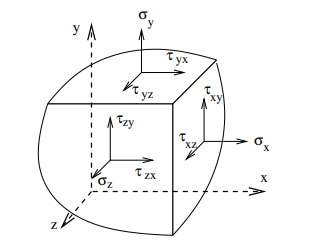
\includegraphics[height=5cm]{assets/figures/framesss/point_stress.png}
    \caption[Napětí v~materiálovém bodě]{Napětí v~materiálovém bodě, převzato z~\cite[3]{teorie_pruznosti}}
    \label{fig:point_stress}
\end{figure}

Uplatněním předpokladu o~vzájemnosti smykových napětí, je možné považovat jen tři smyková napětí za nezávislá \cite[3]{teorie_pruznosti}.

\begin{equation}
    \begin{aligned}
        \gls{tau_i}[\gls{x}\gls{y}] = \gls{tau_i}[\gls{y}\gls{x}], \\
        \gls{tau_i}[\gls{y}\gls{z}] = \gls{tau_i}[\gls{z}\gls{y}], \\
        \gls{tau_i}[\gls{x}\gls{z}] = \gls{tau_i}[\gls{z}\gls{x}].
    \end{aligned}
\end{equation}

Složky lze zapsat v~podobě vektoru napětí

\begin{equation}
    \gls{sigma} 
    =
    \begin{Bmatrix}
        \gls{sigma_i}[\gls{x}] &
        \gls{sigma_i}[\gls{y}] &
        \gls{sigma_i}[\gls{z}] &
        \gls{tau_i}[\gls{y}\gls{z}] &
        \gls{tau_i}[\gls{z}\gls{x}] &
        \gls{tau_i}[\gls{x}\gls{y}]
    \end{Bmatrix}^\mathrm{T}.
\end{equation}

\subsection{Přehled základních rovnic}

\subsubsection*{Geometrické rovnice}
Tělesa mění z~nejrůznějších příčin svůj tvar a objem -- deformují se. Pro deformaci elementárního kvádru jsou typické dva základní geometricko-deformační modely. První předpokládá protažení hran kvádru ve směrech souřadnicových os při zachování pravých úhlů mezi stěnami a druhý model se vyznačuje změnami pravých úhlů mezi stěnami kvádru při zachování délek hran \cite[9]{prpe10}. Na obr. \ref{fig:elementary_block} je pro názornost nakreslen pouze průmět kvádru do roviny \gls{x}\gls{y}.

\begin{figure}[H]
    \begin{tikzpicture}[>={Stealth[inset=0pt,length=8pt,angle'=28,round]}]

    \draw[->] (-0.5, -0.5) -- (8.5, -0.5) node[above] {$\gls{x}, \gls{u_i}[ ]$};
    \draw[->] (-0.5, -0.5) -- (-0.5, 7) node[left] {$\gls{y}, \gls{v_i}[ ]$};

    \coordinate (A_u) at (2.5, 2.5);
    \coordinate (B_u) at (6.5, 2.5);
    \coordinate (C_u) at (6.5, 5);
    \coordinate (D_u) at (2.5, 5);

    
    \coordinate (A_bar) at (2.5, 2.5);
    \coordinate (B_bar) at (7.5, 3.5); 
    \coordinate (C_bar) at (8.5, 7);
    \coordinate (D_bar) at (3.5, 6);

    \draw[draw=ctublue, line width=0.5mm, fill=ctulightblue!30] (A_bar) -- (B_bar) -- (C_bar) -- (D_bar) -- cycle;
    \draw[dotted, draw=ctublue, line width=0.25mm] (A_u) rectangle (C_u);

    \node[above right, color=ctublue] (A_bar_txt) at (A_bar) {$\mathrm{A'}$};
    \node[above left, color=ctublue] (B_bar_txt) at (B_bar) {$\mathrm{B'}$};
    \node[below left, color=ctublue] (C_bar_txt) at (C_bar) {$\mathrm{C'}$};
    \node[below right, color=ctublue] (D_bar_txt) at (D_bar) {$\mathrm{D'}$};
    
    \coordinate (A) at (1, 1);
    \coordinate (B) at (5, 1);
    \coordinate (C) at (5, 3.5);
    \coordinate (D) at (1, 3.5);

    \node at (A) [below left] {A};
    \node at (B) [below right] {B};
    \node at (C) [above right] {C};
    \node at (D) [above left] {D};

    \draw[draw=black, line width=0.5mm] (A) rectangle (C);
    
    \draw[|<->|, draw=black] (1, 0.25) -- node[above] {$\dd{\gls{x}}$} ++ (4, 0);
    \draw[|<->|, draw=black] (0.25, 1) -- node[left] {$\dd{\gls{y}}$} ++(0, 2.5);


    \draw[|<->|, draw=black] (1,1.75) -- node[above left] {\gls{u_i}[ ]} ++(1.5, 0);
    \draw[<->|, draw=black] (2.5, 1.75) -- node[above] {$\dd{\gls{x}}$} ++ (4, 0);
    \draw[<->|, draw=black] (6.5, 1.75) -- node[above] {$\pdv{\gls{u_i}[ ]}{\gls{x}}\dd{\gls{x}}$} ++(1, 0);

    \draw[<->|, draw=black] (2, 1) -- node[below left] {\gls{v_i}[ ]} ++(0, 1.5);
    \draw[<->|, draw=black] (2, 2.5) -- node[left] {$\dd{\gls{y}}$} ++(0, 2.5);
    \draw[<->|, draw=black] (2, 5) -- node[left] {$\pdv{\gls{v_i}[ ]}{\gls{y}}\dd{\gls{y}}$} ++(0, 1);

    \draw[|<->|, draw=black] (8, 2.5) -- node[right] {$\pdv{\gls{v_i}[ ]}{\gls{x}}\dd{\gls{x}}$} ++(0, 1);

    \draw[|<->|, draw=black] (8, 2.5) -- node[right] {$\pdv{\gls{v_i}[ ]}{\gls{x}}\dd{\gls{x}}$} ++(0, 1);
    \draw[|<->|, draw=black] (2.5, 6.5) -- node[above] {$\pdv{\gls{u_i}[ ]}{\gls{y}}\dd{\gls{y}}$} ++(1, 0);

    \draw[|<->|,domain=0:11.31, draw=black] plot ({2.5+3.5*cos(\x)}, {2.5+3.5*sin(\x)});
    \node at (5.7, 2.8) {$\alpha$};

    \draw[|<->|, domain=90:90-15.95, draw=black] plot ({2.5+2.2*cos(\x)}, {2.5+2.2*sin(\x)});
    \node at (2.75, 4.3) {$\beta$};

\end{tikzpicture}
    \caption[Deformace elementárního kvádru]{Deformace elementárního kvádru, podle \cite[obr. 1.2]{teorie_pruznosti}}
    \label{fig:elementary_block}
\end{figure}

Prodloužení kvádru ve směru \gls{x} můžeme vyjářit následovně

\begin{equation}
    \gls{eps_i}[x] 
    = 
    \frac{|\mathrm{A'B'}| - |\mathrm{AB}|}{|\mathrm{AB}|}
    =
    \frac{\left(\dd{\gls{x}} + \pdv{\gls{u_i}[ ]}{\gls{x}} \dd{\gls{x}}\right) - \dd{\gls{x} }}{\dd{\gls{x}}}
    =
    \pdv{\gls{u_i}[ ]}{\gls{x}}.
\end{equation}

Analogicky lze získat vztahy pro \gls{eps_i}[\gls{y}] a \gls{eps_i}[\gls{z}]. Shrnutí vztahů pro poměrné prodloužení ve směru souřadnicových os je uvedeno v~\ref{eq:normal_strain}.

\begin{equation}
    \label{eq:normal_strain}
    \begin{aligned}
        \gls{eps_i}[\gls{x}] & = \pdv{\gls{u_i}[ ]}{\gls{x}}, \\
        \gls{eps_i}[\gls{y}] & = \pdv{\gls{v_i}[ ]}{\gls{y}}, \\
        \gls{eps_i}[\gls{z}] & = \pdv{\gls{w_i}[ ]}{\gls{z}}.
    \end{aligned}
\end{equation}

Smykové zkosení je možné stanovit na základě určení velikostí úhlů $\alpha$ a $\beta$ na obr. \ref{fig:elementary_block}, zavedeme předpoklad, že $\tan{\alpha} = \alpha$, $\tan{\beta}=\beta$, $\pdv{\gls{u_i}[ ]}{\gls{x}} \dd{\gls{x}} = 0$ a $\pdv{\gls{v_i}[ ]}{\gls{y}}\dd{\gls{y}} = 0$.

\begin{equation}
    \gls{gamma_i}[\gls{x}\gls{y}]
    =
    \alpha + \beta
    \approx
    \frac{\pdv{\gls{v_i}[ ]}{\gls{x}}\dd{\gls{x}}}{\dd{\gls{x}}}
    +
    \frac{\pdv{\gls{u_i}[ ]}{\gls{y}}\dd{\gls{y}}}{\dd{\gls{y}}}
    =
    \pdv{\gls{v_i}[ ]}{\gls{x}} + \pdv{\gls{u_i}[ ]}{\gls{y}}
    .
\end{equation}

Analogicky lze zapsat vztahy pro zbývající smyková zkosení

\begin{equation}
    \begin{aligned}
        \gls{gamma_i}[\gls{x}\gls{y}] & = \gls{gamma_i}[\gls{y}\gls{x}] = \pdv{\gls{v_i}[ ]}{\gls{x}} + \pdv{\gls{u_i}[ ]}{\gls{y}}, \\
        \gls{gamma_i}[\gls{y}\gls{z}] & = \gls{gamma_i}[\gls{z}\gls{y}] = \pdv{\gls{w_i}[ ]}{\gls{y}} + \pdv{\gls{v_i}[ ]}{\gls{z}}, \\
        \gls{gamma_i}[\gls{z}\gls{x}] & = \gls{gamma_i}[\gls{x}\gls{z}] = \pdv{\gls{u_i}[ ]}{\gls{z}} + \pdv{\gls{w_i}[ ]}{\gls{x}}.
    \end{aligned}
\end{equation}

\subsubsection*{Fyzikální rovnice}

Jako fyzikální vztahy se označují vztahy mezi napětím a poměrnými deformacemi. Jak je známo z~pružnosti, poměr mezi podélnou a příčnou změnou délky tělesa je konstantní a je popsán Poissonovým součinitelem \gls{nu}. Potom je na místě předpokládat, že velikost poměrného prodloužení \gls{eps_i}[\gls{x}] bude ovlivněna nejen napětím \gls{sigma_i}[\gls{x}], ale v~závislosti na hodnotě \gls{nu} také napětím ve směrech \gls{y} a \gls{z} \cite[7]{teorie_pruznosti}

\begin{equation}
    \gls{eps_i}[\gls{x}] = \frac{1}{\gls{E}} \left[ \gls{sigma_i}[\gls{x}] - \gls{nu} (\gls{sigma_i}[\gls{y}] + \gls{sigma_i}[\gls{z}])  \right].
\end{equation}

U~smyku lze předpokládat, že vztah mezi smykovým napětím \gls{tau_i}[ij] a zkosením \gls{gamma_i}[ij] bude lineární

\begin{equation}
    \gls{gamma_i}[ij] = \frac{\gls{tau_i}[ij]}{2 \gls{G}}.
\end{equation}

Fyzikální vztahy pro pružné těleso v~prostoru můžeme zapsat ve tvaru

\begin{equation}
    \begin{aligned}
        \gls{eps_i}[\gls{x}] & = \frac{1}{\gls{E}} \left[ \gls{sigma_i}[\gls{x}] - \gls{nu} (\gls{sigma_i}[\gls{y}] + \gls{sigma_i}[\gls{z}])  \right], 
        & \quad \gls{gamma_i}[\gls{y}\gls{z}] & = \frac{\gls{tau_i}[\gls{y}\gls{z}]}{2 \gls{G}}, \\
        \gls{eps_i}[\gls{y}] & = \frac{1}{\gls{E}} \left[ \gls{sigma_i}[\gls{y}] - \gls{nu} (\gls{sigma_i}[\gls{x}] + \gls{sigma_i}[\gls{z}])  \right],
        & \quad \gls{gamma_i}[\gls{x}\gls{z}] & = \frac{\gls{tau_i}[\gls{x}\gls{z}]}{2 \gls{G}}, \\
        \gls{eps_i}[\gls{z}] & = \frac{1}{\gls{E}} \left[ \gls{sigma_i}[\gls{z}] - \gls{nu} (\gls{sigma_i}[\gls{y}] + \gls{sigma_i}[\gls{x}])  \right], 
        & \quad \gls{gamma_i}[\gls{x}\gls{y}] & = \frac{\gls{tau_i}[\gls{x}\gls{y}]}{2 \gls{G}}.
    \end{aligned}
\end{equation}

\subsubsection*{Statické rovnice}
V~případě pružného tělesa je vhodné napsat silové podmínky rovnováhy na vyjmutém diferenciálním objemu o~rozměrech $\dd{\gls{x}}$, $\dd{\gls{y}}$, $\dd{\gls{z}}$, který je zobrazen na obrázku \ref{fig:stresses} \cite[6]{teorie_pruznosti}.

Pro lepší přehlednost jsou napětí označená jako $\gls{sigma_i}[i]'$ a $\gls{tau_i}[ij]'$ napětí změněná o~přírůstek na diferenciálním rozměru objemu, tedy například

\begin{equation}
    \label{eq:equilibrium_eq_helpers}
    \gls{sigma_i}[\gls{x}]' = \gls{sigma_i}[\gls{x}] + \pdv{\gls{sigma_i}[\gls{x}]}{\gls{x}} \dd{\gls{x}},
    \quad
    \gls{tau_i}[\gls{x}\gls{y}]' = \gls{tau_i}[\gls{x}\gls{y}] + \pdv{\gls{tau_i}[\gls{x}\gls{y}]}{\gls{y}} \dd{\gls{y}}, \, \dots
\end{equation}

\begin{figure}[H]
    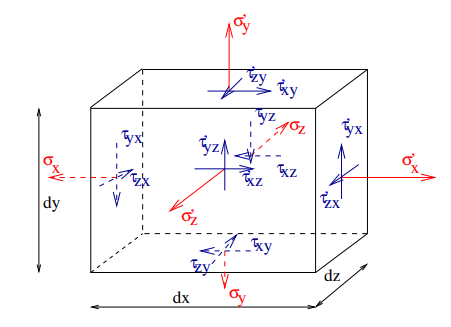
\includegraphics[height=6cm]{assets/figures/framesss/stresses.png}
    \caption[Napětí na diferenciálním výseku tělesa]{Napětí na diferenciálním výseku tělesa, převzato z~\cite[5]{teorie_pruznosti}}
    \label{fig:stresses}
\end{figure}

Výslednice napětí \gls{sigma_i}[\gls{x}] se získá vynásobením napětí a plochy na které působí,

\begin{equation}
    F_{\gls{sigma_i}[ ],\gls{x}} = \gls{sigma_i}[\gls{x}] \dd{\gls{y}} \dd{\gls{z}}.
\end{equation}

Silovou podmínku rovnováhy ve směru osy \gls{x} je možné zapsat jako

\begin{equation}
    \label{eq:equilibrium_eq}
    \sum{F_{i,\gls{x}}} = (\gls{sigma_i}[\gls{x}]' - \gls{sigma_i}[\gls{x}]) \dd{\gls{y}} \dd{\gls{z}}
    + (\gls{tau_i}[\gls{x}\gls{y}]' - \gls{tau_i}[\gls{x}\gls{y}]) \dd{\gls{x}} \dd{\gls{z}}
    + (\gls{tau_i}[\gls{x}\gls{z}]' - \gls{tau_i}[\gls{x}\gls{z}]) \dd{\gls{x}} \dd{\gls{y}} = 0.
\end{equation}

Rozepsáním rovnice \ref{eq:equilibrium_eq} pomocí vztahů \ref{eq:equilibrium_eq_helpers} dostaneme výraz

\begin{equation}
    \begin{aligned}
        & \left(
            \gls{sigma_i}[\gls{x}] 
            - \gls{sigma_i}[\gls{x}] 
            - \pdv{\gls{sigma_i}[\gls{x}]}{\gls{x}} \dd{\gls{x}}
        \right) \dd{\gls{y}} \dd{\gls{z}} \\
        & +
        \left(
            \gls{tau_i}[\gls{x}\gls{y}]
            - \gls{tau_i}[\gls{x}\gls{y}]
            - \pdv{\gls{tau_i}[\gls{x}\gls{y}]}{\gls{y}} \dd{\gls{y}}
        \right) \dd{\gls{x}} \dd{\gls{z}} \\
        & +
        \left(
            \gls{tau_i}[\gls{x}\gls{z}]
            - \gls{tau_i}[\gls{x}\gls{z}]
            - \pdv{\gls{tau_i}[\gls{x}\gls{z}]}{\gls{z}} \dd{\gls{z}}
        \right) \dd{\gls{x}} \dd{\gls{y}}
        = 0,
    \end{aligned}
\end{equation}

který lze dále upravit na

\begin{equation}
    \pdv{\gls{sigma_i}[\gls{x}]}{\gls{x}}
    +
    \pdv{\gls{tau_i}[\gls{x}\gls{y}]}{\gls{y}}
    +
    \pdv{\gls{tau_i}[\gls{x}\gls{z}]}{\gls{z}}
    = 0.
\end{equation}

Obdobně lze napsat podmínky rovnováhy o~pro směry \gls{y} a \gls{z}. Takto sestavené rovnice doplníme o~objemové síly $X$, $Y$ a $Z$, působící ve směrech jednotlivých souřadnicových os, získáme výsledný tvar podmínek rovnováhy,

\begin{equation}
    \begin{aligned}
        \pdv{\gls{sigma_i}[\gls{x}]}{\gls{x}}
        +
        \pdv{\gls{tau_i}[\gls{x}\gls{y}]}{\gls{y}}
        +
        \pdv{\gls{tau_i}[\gls{x}\gls{z}]}{\gls{z}}
        + X & = 0, \\
        \pdv{\gls{tau_i}[\gls{x}\gls{y}]}{\gls{x}}
        +
        \pdv{\gls{sigma_i}[\gls{y}]}{\gls{y}}
        +
        \pdv{\gls{tau_i}[\gls{y}\gls{z}]}{\gls{z}}
        + Y & = 0, \\
        \pdv{\gls{tau_i}[\gls{z}\gls{x}]}{\gls{x}}
        +
        \pdv{\gls{tau_i}[\gls{z}\gls{y}]}{\gls{y}}
        +
        \pdv{\gls{sigma_i}[\gls{z}]}{\gls{z}}
        + Z~& = 0.
    \end{aligned}
\end{equation}

\subsection{Okrajové podmínky}

Složky napětí \gls{sigma} i složky posunutí \gls{eps} musí vyhovovat okrajovým podmínkám předepsaným na hranici tělesa $\gls{gamma} = \gls{gamma_p} + \gls{gamma_u}$.

\subsubsection*{Statické okrajové podmínky}
Statické okrajové podmínky tvoří soustavu tří lineárních algebraických rovnic a vyžadují požadavek rovnováhy pole napětí \gls{sigma} s~předepsaným zatížením \gls{p_bar} na části hranice \gls{gamma_p} \cite[35]{prpe10}. V~maticovém tvaru je lze zapsat

\begin{equation}
    \begin{bmatrix}
        n_{\gls{x}} & 0 & 0 & 0 & n_{\gls{z}} & n_{\gls{y}} \\
        0 & n_{\gls{y}} & 0 & n_{\gls{z}} & 0 & n_{\gls{x}} \\
        0 & 0 & n_{\gls{z}} & n_{\gls{y}} & n_{\gls{z}} & 0
    \end{bmatrix}
    \begin{Bmatrix}
        \gls{sigma_i}[\gls{x}] \\
        \gls{sigma_i}[\gls{y}] \\
        \gls{sigma_i}[\gls{z}] \\
        \gls{tau_i}[\gls{y}\gls{z}] \\
        \gls{tau_i}[\gls{z}\gls{x}] \\
        \gls{tau_i}[\gls{x}\gls{y}]
    \end{Bmatrix}
    =
    \begin{Bmatrix}
        \overline{p}_{\gls{x}} \\
        \overline{p}_{\gls{y}} \\
        \overline{p}_{\gls{z}} \\ 
    \end{Bmatrix},
\end{equation}

neboli

\begin{equation}
    \label{eq:static_boundary_conditions}
    \gls{normal_matrix} \gls{sigma} = \gls{p_bar} \quad \text{na \gls{gamma_p}}.
\end{equation}


\subsubsection*{Kinematické okrajové podmínky}
Kinematické (geometrické) okrajové podmínky se vztahují na část hranice \gls{gamma_u}, kde jsou předepsány posuny $\gls{u_bar} = \begin{Bmatrix}
    \overline{\gls{u_i}[ ]} & \overline{\gls{v_i}[ ]} & \overline{\gls{w_i}[ ]}
\end{Bmatrix}^{\mathrm{T}}$ a mají tvar

\begin{equation}
    \gls{u} = \gls{u_bar} \quad \text{na \gls{gamma_u}}.
\end{equation}

\subsection{Shrnutí}

Pro úplný popis chování pružného tělesa je v~každém jeho bodě potřeba získat hodnoty 15 neznámých veličin, 3 složky posunutí \gls{u}, 6 složek deformací \gls{eps} a 6 složek napětí \gls{sigma}. K~jejich vypočtení máme k~dispozici 15 rovnic, 6 geometrických rovnic, 6 fyzikálních rovnic a 3 statické rovnice (podmínky rovnováhy) \cite[8]{teorie_pruznosti}.

Zmíněné rovnice lze zapsat v~kompaktním tvaru:
\begin{alignat}{2}
    \text{statické~rovnice} \quad && \boldsymbol\partial \gls{sigma}^\mathrm{T} + \gls{X_bar} &= \matr{0}, \label{eq:equilibrium_equations}\\
    \text{fyzikální~rovnice} \quad && \gls{sigma} &= \gls{D} \gls{eps}, \label{eq:constitutive_equations}\\
    \text{geometrické~rovnice} \quad && \gls{eps} &= \boldsymbol\partial{\gls{u}} \label{eq:kinematic_equations},
\end{alignat}
kde
\begin{alignat*}{2}
    & \text{\glsdesc{u}} 
    && \quad \gls{u}
        = 
        \begin{Bmatrix}
            \gls{u_i}[ ] & \gls{v_i}[ ] & \gls{w_i}[ ]
        \end{Bmatrix}^\mathrm{T},
    \\
    & \text{\glsdesc{eps}} 
    && \quad \gls{eps}
        = \begin{Bmatrix}
            \gls{eps_i}[\gls{x}] &
            \gls{eps_i}[\gls{y}] &
            \gls{eps_i}[\gls{z}] &
            \gls{gamma_i}[\gls{x}\gls{y}] &
            \gls{gamma_i}[\gls{y}\gls{z}] &
            \gls{gamma_i}[\gls{z}\gls{x}]
        \end{Bmatrix}^\mathrm{T},
    \\
    %& \text{\glsdesc{D}}
    %&& \quad \gls{D} =
    %\\
    & \text{\glsdesc{sigma}}
    && \quad \gls{sigma}
        = \begin{Bmatrix}
            \gls{sigma_i}[\gls{x}] &
            \gls{sigma_i}[\gls{y}] &
            \gls{sigma_i}[\gls{z}] &
            \gls{tau_i}[\gls{x}\gls{y}] &
            \gls{tau_i}[\gls{y}\gls{z}] &
            \gls{tau_i}[\gls{z}\gls{x}]
        \end{Bmatrix}^\mathrm{T},
    \\
    & \text{\glsdesc{X_bar}}
    && \quad \gls{X_bar}
        = \begin{Bmatrix}
            $X$ & $Y$ & $Z$
        \end{Bmatrix}^\mathrm{T},
    \\ 
    & \text{operátorová matice}
    && \quad \boldsymbol{\partial}
        = \begin{bmatrix}
            \pdv{\gls{x}} & 0 & 0 & 0 & \pdv{\gls{z}} & \pdv{\gls{y}} \\
            0 & \pdv{\gls{y}} & 0 & \pdv{\gls{z}} & 0 & \pdv{\gls{x}} \\
            0 & 0 & \pdv{\gls{z}} & \pdv{\gls{y}} & \pdv{\gls{x}} & 0
        \end{bmatrix}^\mathrm{T},
    \\
    & \text{nulový vektor}
    && \quad \matr{0} = \begin{Bmatrix}
        0 & 0 & 0
    \end{Bmatrix}^\mathrm{T}.
\end{alignat*}

Postupný dosazením \ref{eq:kinematic_equations} a \ref{eq:constitutive_equations} do \ref{eq:equilibrium_equations} získáme silné řešení ve tvaru

\begin{equation}
    \label{eq:strong_form}
    \partial^{\mathrm{T}} \gls{D} \partial{\gls{u}} + \gls{X_bar} = \matr{0}.
\end{equation}

\begin{figure}[H]
    \begin{tikzpicture}[>={Stealth[inset=0pt,length=8pt,angle'=28,round]}]
        \tikzstyle{box} = [rectangle, minimum width=1cm, minimum height=1cm, text centered, draw=black, fill=ctulightblue!30]
    
        \node (displacement) [box] {\gls{u}};
        \node (strain) [box, below=3 cm of displacement] {\gls{eps}};
        \node (stress) [box, right=6 cm of strain] {\gls{sigma}};
        \node (forces) [box, above=3 cm of stress] {\gls{X_bar}};
    
        \draw[->] (displacement) -- node[fill=white] {$\gls{eps} = \partial{\gls{u}}$} (strain);
        \draw[->] (strain) -- node[fill=white] {$\gls{sigma} = \gls{D} \gls{eps}$} (stress);
        \draw[->] (stress) -- node[fill=white] {$\partial^{\mathrm{T}}\gls{sigma} + \gls{X_bar} = \matr{0}$} (forces);
        \draw[->] (forces) -- node[fill=white] (A) {$\partial^{\mathrm{T}} \gls{D} \partial{\gls{u}} + \gls{X_bar} = \matr{0}$} (displacement);
        \node[below=0.1cm of A] (B) {\gls{u} = \gls{u_bar} \quad \text{na \gls{gamma_u}}};
        \node[below=0.1cm of B] {\gls{normal_matrix} \gls{sigma} = \gls{p_bar} \quad \text{na \gls{gamma_p}}};
    
    \end{tikzpicture}
    \caption[Schéma vztahů základních rovnic teorie pružnosti a silného řešení]{Schéma vztahů základních rovnic teorie pružnosti a silného řešení, podle \cite[obr. 1.2]{fem_lourenco}}
    \label{fig:elasticity_diagram}
\end{figure}


\begin{citeQuote}{prpe10}[36]
    S~přesným řešením systému podmínečných rovnic se v~inženýrské praxi setkáváme poměrně zřídka. S~výjimkou několika speciálních typů konstrukcí, jako jsou prutové soustavy nebo rotačně symetrické a symetricky zatížené prostorové konstrukce (např. válcové, kulové ap.), je zpravidla třeba použít řešení přibližných.
\end{citeQuote}

\begin{citeQuote}{fem_lourenco}[kap. 1.1]
    According to solid mechanics, the solution must satisfy this set of differential equations with additional constraints (leading to the so called Boundary Value Problem). Closed-form solutions, such as ${\gls{u}(\gls{x_})=\begin{bmatrix}
        \gls{u_i}[ ](\gls{x_}) & \gls{v_i}[ ](\gls{x_}) & \gls{w_i}[ ](\gls{x_})
    \end{bmatrix}^{\mathrm{T}}}$ defined over the entire problem domain, are possible only when simple geometries and loadings are considered.
\end{citeQuote}
\section{Princip virtuálních prací}

Princip virtuálních prací a variační principy mechaniky jsou základem většiny přibližných metod mechaniky. Princip virtuálních prací lze dělit na princip virtuálních posunutí a princip virtuálních sil.

Publikace \cite[53]{prpe20} uvádí následující definice:
\begin{definition}[Virtuální posun]
    \label{def:virtual_displacement}
    Libovolný možný posun elementu mechanické soustavy, který je v~souladu s~jejími pohybovými možnostmi. Elementem mechanické soustavy rozumíme jakoukoliv její část, jež je s~ostatními částmi spojena vazbami.
\end{definition}

\begin{definition}[Virtuální deformace]
    Jsou odvozeny z~virtuálních posunů pomocí geometrických rovnic. Virtuální posuny i deformace nenarušují vazby soustavy. Jsou fiktivní, myšlené a uděleme je elementům soustavy bez ohledu na síly a napětí, které na ně působí.
\end{definition}

\begin{definition}[Virtuální síla]
    Duální protějšek virtuálního posunu. Je to síla, kterou na soustavu umisťujeme nezávisle na skutečných posunech.
\end{definition}

\begin{definition}[Virtuální napětí]
    Fiktivní, myšlené veličiny. Jsou stanoveny tak, aby v~každém bodě tělesa, které je zatíženo virtuálními silami, byla zajištěna rovnováha.
\end{definition}

Předpokládejme, že se těleso nachází v~jisté rovnovážné konfiguraci, která je jednoznačně popsána vektorovým polem posunutí $$\gls{u} = \begin{Bmatrix}
    \gls{u_i}[ ] & \gls{v_i}[ ] & \gls{w_i}[ ]
\end{Bmatrix}^\mathrm{T},$$ tenzorovým polem deformace $$\gls{eps} = \begin{Bmatrix}
    \gls{eps_i}[\gls{x}] & \gls{eps_i}[\gls{y}] & \gls{eps_i}[\gls{z}] & \gls{gamma_i}[\gls{y}\gls{z}] & \gls{gamma_i}[\gls{z}\gls{x}] & \gls{gamma_i}[\gls{x}\gls{y}]
\end{Bmatrix}^\mathrm{T},$$ a tenzorovým polem napětí $$\gls{sigma} = \begin{Bmatrix}
    \gls{sigma_i}[\gls{x}] & \gls{sigma_i}[\gls{y}] & \gls{sigma_i}[\gls{z}] & \gls{tau_i}[\gls{y}\gls{z}] & \gls{tau_i}[\gls{z}\gls{x}] & \gls{tau_i}[\gls{x}\gls{y}]
\end{Bmatrix}^\mathrm{T}.$$

Dále předpokládejme, že každému bodu tělesa je udělen malý virtuální posun 
$$\gls{delta}\gls{u} = \begin{Bmatrix}
    \gls{delta}\gls{u_i}[ ] & \gls{delta}\gls{v_i}[ ] & \gls{delta}\gls{w_i}[ ]
\end{Bmatrix}^\mathrm{T},$$
který jej vychýlí z~původní polohy v~rovnovážné konfiguraci. Funkce \gls{delta}\gls{u_i}[ ], \gls{delta}\gls{v_i}[ ] a \gls{delta}\gls{w_i}[ ] jsou ve smyslu definice \ref{def:virtual_displacement} spojité a mají spojité první parciální derivace podle proměnných \gls{x}, \gls{y} a \gls{z}. Výsledné posuny $\left( \gls{u} + \gls{delta}\gls{u} \right)$ a odvozené deformace $\left( \gls{eps} + \gls{delta}\gls{eps} \right)$ se nazývají kinematicky přípustné.

Připojením virtuálních objemových sil 
\begin{equation*}
    \gls{delta}\gls{X_bar} = \begin{Bmatrix}
        \gls{delta} \overline{X} & \gls{delta}\overline{Y} & \gls{delta}\overline{Z}
    \end{Bmatrix}^\mathrm{T}
\end{equation*}
a virtuálních povrchových sil 
\begin{equation*}
    \gls{delta}\gls{p_bar} = \begin{Bmatrix}
        \gls{delta} p_{\gls{x}} & \gls{delta} p_{\gls{y}} & \gls{delta} p_{\gls{z}}
    \end{Bmatrix}^\mathrm{T},
\end{equation*} 
změníme stav zatížení tělesa a připojením virtuálních napětí $$\gls{delta}\gls{sigma} = \begin{Bmatrix}
    \gls{delta}\gls{sigma_i}[\gls{x}] & \gls{delta}\gls{sigma_i}[\gls{y}] & \gls{delta}\gls{sigma_i}[\gls{z}] & \gls{delta}\gls{tau_i}[\gls{y}\gls{z}] & \gls{delta}\gls{tau_i}[\gls{z}\gls{x}] & \gls{delta}\gls{tau_i}[\gls{x}\gls{y}]
\end{Bmatrix}^\mathrm{T},$$ jeho napjatost.

Nemá-li být narušena rovnováha tělesa, musí v~každém bodě platit rovnice \ref{eq:equilibrium_equations}

\begin{equation}
    \boldsymbol\partial \gls{delta}\gls{sigma} + \gls{delta}\gls{X_bar} = \matr{0},
\end{equation}

a na hranici tělesa \gls{gamma}

\begin{equation}
    \gls{normal_matrix} \gls{delta}\gls{sigma} - \gls{delta}\gls{p_bar} = \matr{0}.
\end{equation}

Výsledné síly $(\gls{X_bar} + \gls{delta}\gls{X_bar})$, $(\gls{p_bar} + \gls{delta}\gls{p_bar})$ a výsledná napětí $(\gls{sigma} + \gls{delta}\gls{sigma})$ se nazývají \textbf{staticky přípustné}.

Princip virtuálních prací lze matematicky zapsat následovně
\begin{equation}
    \label{eq:principle_of_virtual_work}
    \small
    \underbrace{
    \int_{\gls{omega}} 
    (\gls{sigma} + \gls{delta}\gls{sigma})^{\mathrm{T}}
    ( \gls{eps} + \gls{delta}\gls{eps} ) 
    \dd{\gls{omega}}}_{\text{virtuální práce vnitřních sil}}
    =
    \underbrace{
    \int_{\gls{omega}}
    (\gls{X_bar} + \gls{delta}\gls{X_bar})^{\mathrm{T}}
    ( \gls{u} + \gls{delta}\gls{u} )
    \dd{\gls{omega}}
    +
    \int_{\gls{gamma}}
    (\gls{p_bar} + \gls{delta}\gls{p_bar})^{\mathrm{T}}
    ( \gls{u} + \gls{delta}\gls{u} )
    \dd{\gls{gamma}}.}_{\text{virtuální práce vnějších sil}}
\end{equation}

Vhodným upravením rovnice \ref{eq:principle_of_virtual_work}, při uvážení vzájemné nezávislosti zavedených virtuálních polí, obdržíme čtyři rovnice, které musí být splněny nezávisle na sobě,

\begin{itemize}
    \item Clapeyronův (divergenční) teorém
    \begin{equation}
        \label{eq:clapeyron}
        \int_{\gls{omega}}\gls{sigma}^{\mathrm{T}} \gls{eps} \dd{\gls{omega}}
        =
        \int_{\gls{omega}}
        \gls{X_bar}^{\mathrm{T}} \gls{u} \dd{\gls{omega}}
        +
        \int_{\gls{gamma}} \gls{p_bar}^{\mathrm{T}} \gls{u} \dd{\gls{gamma}},
    \end{equation}
    \item princip virtuálních posunutí
    \begin{equation}
        \label{eq:principle_of_virtual_displacement}
        \int_{\gls{omega}}\gls{sigma}^{\mathrm{T}} \gls{delta}\gls{eps} \dd{\gls{omega}}
        =
        \int_{\gls{omega}}
        \gls{X_bar}^{\mathrm{T}} \gls{delta}\gls{u} \dd{\gls{omega}}
        +
        \int_{\gls{gamma}} \gls{p_bar}^{\mathrm{T}} \gls{delta}\gls{u} \dd{\gls{gamma}},
    \end{equation}
    \item princip virtuálních sil
    \begin{equation}
        \label{eq:principle_of_virtual_forces}
        \int_{\gls{omega}} \gls{delta}\gls{sigma}^{\mathrm{T}} \gls{eps} \dd{\gls{omega}}
        =
        \int_{\gls{omega}}
        \gls{delta}\gls{X_bar}^{\mathrm{T}} \gls{u} \dd{\gls{omega}}
        +
        \int_{\gls{gamma}} \gls{delta}\gls{p_bar}^{\mathrm{T}} \gls{u} \dd{\gls{gamma}},
    \end{equation}
    \item čtvrtá rovnice, která nemá bezprostřední využití, ve tvaru
    \begin{equation}
        \int_{\gls{omega}} \gls{delta}\gls{sigma}^{\mathrm{T}} \gls{delta}\gls{eps} \dd{\gls{omega}}
        =
        \int_{\gls{omega}}
        \gls{delta}\gls{X_bar}^{\mathrm{T}} \gls{delta}\gls{u} \dd{\gls{omega}}
        +
        \int_{\gls{gamma}} \gls{delta}\gls{p_bar}^{\mathrm{T}} \gls{delta}\gls{u} \dd{\gls{gamma}}.
    \end{equation}
\end{itemize}


\subsection{Princip virtuálních posunutí}

Dále se budeme zabývat principem virtuálních posunutí, ze kterého odvodíme algoritmus deformační metody.

Uvažujme takové virtuální posuny \gls{delta}\gls{u}, které nenarušují kinematické okrajové podmínky
\begin{equation}
    \label{eq:virtual_displacements_boundary}
    \gls{delta}\gls{u} = \matr{0}, \quad \text{na hranici \gls{gamma_u}},
\end{equation}

a zároveň splňují geometrické rovnice uvnitř tělesa
\begin{equation}
    \label{eq:pvd_geometric_eqs}
    \gls{delta}\gls{eps} = \boldsymbol{\partial}\gls{delta}\gls{u}, \quad \text{uvnitř tělesa \gls{omega}}.
\end{equation}

Rovnici \ref{eq:principle_of_virtual_displacement} zapíšeme s~přihlédnutím k~\ref{eq:virtual_displacements_boundary},
\begin{equation}
    \label{eq:pvd_start}
    \int_{\gls{omega}}\gls{sigma}^{\mathrm{T}} \gls{delta}\gls{eps} \dd{\gls{omega}}
    =
    \int_{\gls{omega}}
    \gls{X_bar}^{\mathrm{T}} \gls{delta}\gls{u} \dd{\gls{omega}}
    +
    \int_{\gls{gamma_p}} \gls{p_bar}^{\mathrm{T}} \gls{delta}\gls{u} \dd{\gls{gamma_p}}.
\end{equation}

Levou stranu rovnice \ref{eq:pvd_start} upravíme dosazením z~rovnice \ref{eq:pvd_geometric_eqs},

\begin{equation}
    \int_{\gls{omega}}\gls{sigma}^{\mathrm{T}} \gls{delta}\gls{eps} \dd{\gls{omega}}
    =
    \int_{\gls{omega}}\gls{sigma}^{\mathrm{T}} \boldsymbol\partial \gls{delta}\gls{u} \dd{\gls{omega}},
\end{equation}

a zintegrujeme per partes, pomocí věty o~integraci tenzorového pole \cite[55]{prpe20},

\begin{equation}
    \label{eq:pvd_per_partes}
    \int_{\gls{omega}}\gls{sigma}^{\mathrm{T}} \boldsymbol\partial \gls{delta}\gls{u} \dd{\gls{omega}}
    =
    \int_{\gls{gamma}} \gls{delta}\gls{u}^{\mathrm{T}} \gls{normal_matrix} \gls{sigma} \dd{\gls{gamma}}
    -
    \int_{\gls{omega}} \gls{delta}\gls{u}^{\mathrm{T}} \boldsymbol\partial \gls{sigma} \dd{\gls{omega}}.
\end{equation}

Dosazením z~rovnice \ref{eq:pvd_per_partes} do původního vztahu \ref{eq:pvd_start} dostaneme rovnici

\begin{equation}
    \int_{\gls{gamma}} \gls{delta}\gls{u}^{\mathrm{T}} \gls{normal_matrix} \gls{sigma} \dd{\gls{gamma}}
    -
    \int_{\gls{omega}} \gls{delta}\gls{u}^{\mathrm{T}} \boldsymbol\partial \gls{sigma} \dd{\gls{omega}}
    =
    \int_{\gls{omega}}
    \gls{X_bar}^{\mathrm{T}} \gls{delta}\gls{u} \dd{\gls{omega}}
    +
    \int_{\gls{gamma_p}} \gls{p_bar}^{\mathrm{T}} \gls{delta}\gls{u} \dd{\gls{gamma_p}},
\end{equation}

rozepsáním prvního integrálu na část s~předepsaným zatížením \gls{gamma_p} a s~předepsanými posuny \gls{gamma_u} dostaneme tvar

\begin{equation}
    \small
    \int_{\gls{gamma_p}} \gls{delta}\gls{u}^{\mathrm{T}} \gls{normal_matrix} \gls{sigma} \dd{\gls{gamma_p}}
    +
    \int_{\gls{gamma_u}} \gls{delta}\gls{u}^{\mathrm{T}} \gls{normal_matrix} \gls{sigma} \dd{\gls{gamma_u}}
    -
    \int_{\gls{omega}} \gls{delta}\gls{u}^{\mathrm{T}} \boldsymbol\partial \gls{sigma} \dd{\gls{omega}}
    =
    \int_{\gls{omega}}
    \gls{X_bar}^{\mathrm{T}} \gls{delta}\gls{u} \dd{\gls{omega}}
    +
    \int_{\gls{gamma_p}} \gls{p_bar}^{\mathrm{T}} \gls{delta}\gls{u} \dd{\gls{gamma_p}},
\end{equation}

kde podle kinematické okrajové podmínky \ref{eq:virtual_displacements_boundary}

\begin{equation*}
    \int_{\gls{gamma_u}} \gls{delta}\gls{u}^{\mathrm{T}} \gls{normal_matrix} \gls{sigma} \dd{\gls{gamma_u}} = 0.
\end{equation*}

Po úpravě dostaneme

\begin{equation}
    \label{eq:pvd}
    \int_{\gls{omega}} \gls{delta}\gls{u}^{\mathrm{T}} 
    (\boldsymbol{\partial} \gls{sigma} + \gls{X_bar})
    \dd{\gls{omega}}
    +
    \int_{\gls{gamma_p}} \gls{delta}\gls{u}^{\mathrm{T}}
    (-\gls{normal_matrix} \gls{sigma}
    +
    \gls{p_bar})
    \dd{\gls{gamma_p}}
    = 0.
\end{equation}

Protože virtuální posuny \gls{delta}\gls{u} jsou libovolné, rovnice \ref{eq:pvd} bude splněna právě tehdy, pokud budou zároveň platit statické rovnice \ref{eq:equilibrium_equations} a statické okrajové podmínky \ref{eq:static_boundary_conditions}. 
\subsection{Přibližné řešení} \label{sec:approximate_solution}

Rovnice \ref{eq:pvd_start} může být použita k přibližnému řešení úlohy teorie pružnosti. Předpokládejme, že neznámé posuny \gls{u}(\gls{x_}) lze aproximovat pomocí

\begin{equation} \label{eq:approx_first}
    \gls{u}(\gls{x_}) \approx \gls{N}(\gls{x_})\gls{d},
\end{equation}
kde
\begin{alignat*}{2}
    & \gls{N}(\gls{x_})     && \quad \text{\glsdesc{N},} \\
    & \gls{d}               && \quad \text{\glsdesc{d}.}
\end{alignat*}

Pomocí geometrických rovnic \ref{eq:kinematic_equations} určíme pole deformace,

\begin{equation}
    \begin{split}
        \gls{eps}(\gls{x_}) &= \boldsymbol\partial\gls{N}(\gls{x_}){\gls{d}} \\
                            &= \gls{B}(\gls{x_}){\gls{d}}.
    \end{split}
\end{equation}

Pole napětí vypočítáme z pole deformace pomocí fyzikálních rovnic \ref{eq:constitutive_equations},

\begin{equation}
    \begin{split}
        \gls{sigma}(\gls{x_}) &= \gls{D} \gls{eps}(\gls{x_}) \\
                             &= \gls{D} \gls{B}(\gls{x_}){\gls{d}}.
    \end{split}
\end{equation}

Virtuální pole posunutí je aproximováno stejnými bázovými funkcemi,

\begin{equation}
    \gls{delta}\gls{u}(\gls{x_}) = \gls{N}(\gls{x_})\gls{delta}\gls{d},
\end{equation}

pole virtuálních deformací je s virtuálními posuny svázáno stejnou maticí \gls{B},

\begin{equation} \label{eq:approx_last}
    \gls{delta}\gls{eps} = \gls{B}(\gls{x_})\gls{delta}\gls{d}.
\end{equation}

Pro zjednodušení v dalším textu budeme matici bázových funkcí $\gls{N}(\gls{x_})$ a matici $\gls{B}(\gls{x_})$ značit pouze jako $\gls{N}$ a $\gls{B}$,  přičemž je třeba mít na paměti, že jsou závislé na $\gls{x_}$.


Dosazením vztahů \ref{eq:approx_first} až \ref{eq:approx_last} do rovnice \ref{eq:pvd_start} obdržíme,

\begin{equation}
    \int_{\gls{omega}} (\gls{D} \gls{B} \gls{d})^{\mathrm{T}} \gls{B} \gls{delta} \gls{d} \dd{\gls{omega}}
    =
    \int_{\gls{omega}} \gls{X_bar}^\mathrm{T} \gls{N} \gls{delta}\gls{d} \dd{\gls{omega}}
    +
    \int_{\gls{gamma_p}} \gls{p_bar}^\mathrm{T} \gls{N} \gls{delta}\gls{d} \dd{\gls{gamma_p}}.
\end{equation}

Úpravou dostaneme tvar,

\begin{equation}
    \gls{d}^\mathrm{T} \underbrace{\int_{\gls{omega}}  \gls{B}^\mathrm{T} \gls{D}^\mathrm{T} \gls{B} \dd{\gls{omega}}}_{\gls{K}^\mathrm{T}} \gls{delta}\gls{d}
    =
    \underbrace{\left(\int_{\gls{omega}} \gls{X_bar}^\mathrm{T} \gls{N} \dd{\gls{omega}}
    +
    \int_{\gls{gamma_p}} \gls{p_bar}^\mathrm{T} \gls{N} \dd{\gls{gamma_p}}\right)}_{\gls{f}^\mathrm{T}} \gls{delta}\gls{d}.
\end{equation}

Rovnici dále přepíšeme pomocí matice tuhosti \gls{K} a vektoru zatížení \gls{f} a upravíme\footnote{
    $\left(\matr{A}\matr{B}\right)^\mathrm{T} = \matr{B}^\mathrm{T} \matr{A}^\mathrm{T}$
    },
\begin{align*}
    \gls{d}^\mathrm{T} \gls{K}^\mathrm{T} \gls{delta}\gls{d} &= \gls{f}^\mathrm{T} \gls{delta} \gls{d} \\
    \gls{delta}\gls{d}^\mathrm{T} \left( \gls{d}^\mathrm{T} \gls{K}^\mathrm{T} \right)^\mathrm{T} &= \gls{delta} \gls{d}^\mathrm{T}  \gls{f} \\
    \gls{delta}\gls{d}^\mathrm{T} \left( \gls{K}\gls{d} - \gls{f} \right) &= 0.
\end{align*}

Protože rovnice musí platit pro libovolné virtuální posunutí \gls{delta}\gls{d}, musí být výraz v závorce nulovým vektorem. Odvodili jsme tedy zobecněné podmínky rovnováhy ve tvaru

\begin{equation}
    \gls{K} \gls{d} - \gls{f} = \matr{0},
\end{equation}

kde \gls{K} je matice tuhosti,

\begin{equation} \label{eq:K}
    \gls{K} = \int_{\gls{omega}} \gls{B}^{\mathrm{T}}\gls{D}\gls{B} \dd{\gls{omega}},
\end{equation}

a \gls{f} je vektor zatížení,

\begin{equation} \label{eq:f}
    \gls{f} = \int_{\gls{omega}} \gls{N}^{\mathrm{T}} \gls{X_bar} \dd{\gls{omega}} + \int_{\gls{gamma_p}} \gls{N}^{\mathrm{T}} \gls{p_bar} \dd{\gls{gamma_p}}.
\end{equation}


\begin{figure}[H]
    \begin{tikzpicture}[>={Stealth[inset=0pt,length=8pt,angle'=28,round]}]
        \tikzstyle{box} = [rectangle, minimum width=1cm, minimum height=1cm, text centered, draw=black, fill=ctulightblue!30]
    
        \node (displacement) [box] {$\gls{u}(\gls{x_}) \approx \gls{N}(\gls{x_})\gls{d}$};
        \node (strain) [box, below=3 cm of displacement] {$\gls{eps}(\gls{x_}) \approx \gls{B}(\gls{x_}) \gls{d}$};
        \node (stress) [box, right=6 cm of strain] {$\gls{sigma}(\gls{x_}) \approx \gls{D} \gls{B}(\gls{x_})\gls{d}$};
        \node (forces) [box, above=3 cm of stress] {$\gls{X_bar}(\gls{x_})$};
    
        \draw[->] (displacement) -- node[fill=white] {$\gls{eps} = \partial{\gls{u}}$} (strain);
        \draw[->] (strain) -- node[fill=white] {$\gls{sigma} = \gls{D} \gls{eps}$} (stress);
        \draw[->] (stress) -- node[fill=white, left=-2.5cm] {$
            \begin{aligned}
                & \forall \left( \gls{delta}\gls{u}, \gls{delta}\gls{eps}\right) | \gls{delta}\gls{eps} = \partial\gls{delta}\gls{u}: \\
                & \int_{\gls{omega}}\gls{sigma}^{\mathrm{T}} \gls{delta}\gls{eps} \dd{\gls{omega}}
                =
                \int_{\gls{omega}}
                \gls{X_bar}^{\mathrm{T}} \gls{delta}\gls{u} \dd{\gls{omega}}
                +
                \int_{\gls{gamma_p}} \gls{p_bar}^{\mathrm{T}} \gls{delta}\gls{u} \dd{\gls{gamma_p}}
            \end{aligned}$
            } (forces);
        \draw[->] (forces) -- node[fill=white] (A) {$\gls{K}\gls{d} - \gls{f} = \matr{0}$} (displacement);
    
    \end{tikzpicture}
    \caption[Schéma vztahů základních rovnic teorie pružnosti a slabého řešení]{Schéma vztahů základních rovnic teorie pružnosti a slabého řešení, podle \cite[obr. 1.3]{fem_lourenco}}
    \label{fig:weak_form_diagram}
\end{figure}
\section{Prutové prvky}

V této části se zaměříme na řešení prutových konstrukcí. Prut je těleso s výrazně převládající délkou nad rozměry průřezu. Dimenzi z pohledu napjatosti budeme redukovat na jednorozměrný problém. 

Přijmeme následující předpoklady,
\begin{itemize}
    \item zatížení působí pouze v rovině \gls{X}\gls{Z}, která je i rovinou symetrie, řešení není funkcí souřadnice \gls{y},
    \item průhyb ve směru osy \gls{z} je po výšce prvku konstantní,
    \item výrazně převládajícím rozměrem je délka prvku \gls{L},
    \item uvažujeme prizmatický prut (s neměnným průřezem po délce prvku),
    \item uvažujeme teorii malých přetvoření,
    \item materiál prutu se chová pružně a je homogenní.
\end{itemize}

\subsubsection*{Vektor posunutí}
Vzhledem k přijatým předpokladům je posun ve směru osy \gls{Y} nulový, zároveň uvažujeme po výšce nestlačitelný prut, to znamená, že posun ve směru osy \gls{z} je závislý pouze na souřadnici \gls{x}. V dalších kapitolách si vystačíme s vektorem posunutí ve tvaru

\begin{equation}
    \gls{u}(\gls{x_}) = \begin{Bmatrix}
        \gls{u_i}[ ](\gls{x}, \gls{z}) &
        \gls{w_i}[ ](\gls{x})
    \end{Bmatrix}{^\mathrm{T}}.
\end{equation}

\subsubsection*{Vektor deformací}
Vektor deformací odpovídající předpokladům má dvě nenulové složky, 

\begin{equation}
    \gls{eps}(\gls{x}, \gls{z})
    = 
    \begin{Bmatrix}
        \gls{eps_i}[\gls{x}](\gls{x}, \gls{z}) &
        \gls{gamma_i}[\gls{z}\gls{x}](\gls{x}, \gls{z})
    \end{Bmatrix}^{\mathrm{T}}
    =
    \begin{Bmatrix}
        \pdv{\gls{u_i}[ ](\gls{x}, \gls{z})}{\gls{x}} &
        \pdv{\gls{u_i}[ ](\gls{x}, \gls{z})}{\gls{z}} + \pdv{\gls{w_i}[ ](\gls{x})}{\gls{x}}
    \end{Bmatrix}^{\mathrm{T}}.
\end{equation}


\subsubsection*{Vektor napětí}

Při analýze prutových konstrukcí je běžné pracovat s vnitřními silami místo s napětím. Vnitřní síly jsou s napětím svázany podmínkami ekvivalence
\begin{align}
    \gls{axial_force}(\gls{x}) &= \int_{\gls{A}} \gls{sigma_i}[\gls{x}] \dd{\gls{A}}, \label{eq:N}\\
    \gls{shear_force}(\gls{x}) &= \int_{\gls{A}} \gls{tau_i}[\gls{x}\gls{z}] \dd{\gls{A}}, \label{eq:V}\\
    \gls{bending_moment}(\gls{x}) &= \int_{\gls{A}} \gls{sigma_i}[\gls{x}] \gls{z} \dd{\gls{A}}, \label{eq:M}
\end{align}
kde $\dd{\gls{A}} = \dd{\gls{y}}\dd{\gls{z}}$.

\subsubsection*{Podmínky rovnováhy}
Podmínky rovnováhy na prvku lze zapsat jako
\begin{align}
    \dv{\gls{axial_force}(\gls{x})}{\gls{x}} + \bar{f}_{\gls{x}}(\gls{x}) &= 0, \\
    \dv{\gls{shear_force}(\gls{x})}{\gls{x}} + \bar{f}_{\gls{z}}(\gls{x}) &= 0, \label{eq:V_equilibrium}\\
    \dv{\gls{bending_moment}(\gls{x})}{\gls{x}} - \gls{shear_force}(\gls{x}) &= 0, \label{eq:M_equilibrium}
\end{align}
kde $\bar{f}_{\gls{x}}(\gls{x})$ a $\bar{f}_{\gls{z}}(\gls{x})$ je zatížení působící po délce prutu.

\subsubsection*{Kinematické podmínky}
Kinematické podmínky jsou dány typem podpory, např. pro vetknutí platí
\begin{equation}
    \gls{u_i}[ ] = 0, \quad \gls{w_i}[ ] = 0, \quad \gls{phi_i}[ ] = 0.
\end{equation}

\subsection{Tažený-tlačený prut}

\begin{figure}[H]
    \newcommand*{\xStart}{0}
\newcommand*{\xEnd}{8}
\newcommand*{\uStart}{1}
\newcommand*{\uEnd}{2}
\newcommand*{\height}{2}
\newcommand*{\xDivisions}{10} % Number of divisions along the x-axis
\newcommand*{\yDivisions}{4}  % Number of divisions along the y-axis

\begin{tikzpicture}[>={Stealth[inset=0pt,length=8pt,angle'=28,round]}, scale=0.8]
    % Draw axes
    \draw[->] (0, 0) -- (11, 0) node[above] {\gls{x}};
    \draw[->] (0, 0) -- (0, 2.5) node[above] {\gls{z}};
    
    % Draw the initial bar
    \draw[black] (\xStart, -\height/2) rectangle (\xEnd, \height/2);

    % Calculate spacing
    \pgfmathsetmacro{\xSpacing}{(\xEnd-\xStart)/\xDivisions}
    \pgfmathsetmacro{\ySpacing}{\height/\yDivisions}
    \pgfmathsetmacro{\xDefDivs}{\xDivisions-1}
    \pgfmathsetmacro{\yDefDivs}{\yDivisions-1}

    %Draw bar grid
    \foreach \i in {1,...,\xDefDivs} {
        \draw[draw=black, dotted] (\xStart + \i*\xSpacing, -\height/2) -- (\xStart + \i*\xSpacing, \height/2); % Vertical grid lines
    }
    \foreach \i in {1,...,\yDefDivs} {
        \draw[draw=black, dotted] (\xStart, -\height/2 + \i*\ySpacing) -- (\xEnd, -\height/2 + \i*\ySpacing); % Horizontal grid lines
    }

    % Draw deformed bar
    \draw[ctublue, thick] (\xStart + \uStart, -\height/2) rectangle (\xEnd + \uEnd, \height/2);
    
    % Draw deformed grid
    \pgfmathsetmacro{\uDelta}{(\uEnd - \uStart)/(\xDivisions)}

    \foreach \i in {1,...,\xDefDivs} {
        \draw[ctulightblue] (\xStart + \i*\xSpacing + \uStart + \i*\uDelta, -\height/2) -- (\xStart + \i*\xSpacing + \uStart + \i*\uDelta, \height/2); % Vertical deformed grid lines
    }
    \foreach \i in {1,...,\yDefDivs} {
        \draw[ctulightblue] (\xStart + \uStart, -\height/2 + \i*\ySpacing) -- (\xEnd + \uEnd, -\height/2 + \i*\ySpacing); % Horizontal deformed grid lines
    }
    % nodes
    \draw[ultra thick] (\xStart, 0) -- (\xEnd, 0);
    \draw[fill=white] (\xStart, 0) circle (.25cm) node[text=black] {$a$};
    \draw[fill=white] (\xEnd, 0) circle (.25cm) node[text=black] {$b$};

    \draw[|->|, draw=ctublue, text=ctublue] (\xStart, +\height/2+0.3) -- node[above] {$u_a$} ++(\uStart, 0);
    \draw[|->|, draw=ctublue, text=ctublue] (\xEnd, +\height/2+0.3) -- node[above] {$u_b$} ++(\uEnd, 0);

    \draw[|<->|, draw=black] (\xStart, -\height/2-0.7) -- node[above] {\gls{L}} (\xEnd, -\height/2-0.7);
    

\end{tikzpicture}
    \caption{Deformovaná konfigurace taženého-tlačeného prutu}
    \label{fig:deformed_bar}
\end{figure}

Tažený-tlačený prut je v rovině dán pomocí dvou uzlů, $a$ a $b$. V každém bodě zavedeme koncové posunutí ve směru lokální osy \gls{x}. Vektor zobecněných posunutí má tvar
\begin{equation}
    \gls{d} = \begin{Bmatrix}
        \gls{u_i}[a] \\
        \gls{u_i}[b]
    \end{Bmatrix}.
\end{equation}

Pomocí vektoru koncových posunutí \gls{d} a matice bázových funkcí \gls{N} budeme aproximovat posunutí $\gls{u_i}[ ](\gls{x})$ libovolného průřezu prvku,
\begin{equation} \label{eq:bar_ux}
    \gls{u_i}[ ](\gls{x}) \approx \gls{N}(\gls{x}) \gls{d}
    = \begin{bmatrix}
        \gls{N_i}[1](\gls{x}) & \gls{N_i}[2](\gls{x})
    \end{bmatrix}
    \begin{Bmatrix}
        \gls{u_i}[a] \\
        \gls{u_i}[b]
    \end{Bmatrix}.
\end{equation}

\subsubsection*{Bázové funkce}

Bázové funkce $\gls{N_i}[i](\gls{x})$ budeme hledat ve tvaru polynomu prvního stupně,
\begin{equation}
    \gls{N_i}[i](\gls{x}) = a_i \gls{x} + b_i,
\end{equation}
kde $a_i$ a $b_i$ jsou zatím neznámé koeficienty. Rozepsáním vztahu \ref{eq:bar_ux} do maticové podoby dostaneme výraz
\begin{equation} \label{eq:bar_ux_matrix}
    \gls{u_i}[ ](\gls{x})
    =
    \begin{bmatrix}
        \gls{x} & 1
    \end{bmatrix}
    \begin{bmatrix}
        a_1 & a_2 \\
        b_1 & b_2
    \end{bmatrix}
    \begin{Bmatrix}
        \gls{u_i}[a] \\
        \gls{u_i}[b]
    \end{Bmatrix}.
\end{equation}


Okrajové podmínky, patrné z obrázku \ref{fig:deformed_bar} jsou
\begin{subequations}
    \begin{equation} \label{eq:bar_ua}
        \gls{u_i}[ ](0) = \gls{u_i}[a], \\        
    \end{equation}
    \begin{equation} \label{eq:bar_ub}
        \gls{u_i}[ ](\gls{L}) = \gls{u_i}[b].
    \end{equation}
\end{subequations}

Dosazením okrajových podmínek \ref{eq:bar_ua} a \ref{eq:bar_ub} do vztahu \ref{eq:bar_ux_matrix} dostaneme soustavu rovnic
\begin{equation}
    \underbrace{
    \begin{bmatrix}
        0 & 1 \\
        \gls{L} & 1
    \end{bmatrix}}_\matr{A}
    \begin{bmatrix}
        a_1 & a_2 \\
        b_1 & b_2
    \end{bmatrix}
    \begin{Bmatrix}
        \gls{u_i}[a] \\
        \gls{u_i}[b]
    \end{Bmatrix} = 
    \begin{Bmatrix}
        \gls{u_i}[a] \\
        \gls{u_i}[b]
    \end{Bmatrix}.
\end{equation}

Přenásobením rovnice zleva maticí $\matr{A}^{-1}$ dostaneme
\begin{equation}
    \begin{bmatrix}
        a_1 & a_2 \\
        b_1 & b_2
    \end{bmatrix}
    \begin{Bmatrix}
        \gls{u_i}[a] \\
        \gls{u_i}[b]
    \end{Bmatrix} 
    = 
    \begin{bmatrix}
        0 & 1 \\
        \gls{L} & 1
    \end{bmatrix}^{-1}
    \begin{Bmatrix}
        \gls{u_i}[a] \\
        \gls{u_i}[b]
    \end{Bmatrix},
\end{equation}
ze které je patrné, že matice koeficientů bázových funkcí se rovná inverzní matici k matici $\matr{A}$,
\begin{equation}
    \begin{bmatrix}
        a_1 & a_2 \\
        b_1 & b_2
    \end{bmatrix}
    =
    \begin{bmatrix}
        -\frac{1}{\gls{L}} & \frac{1}{\gls{L}} \\
        1 & 0
    \end{bmatrix}.
\end{equation}

Bázové funkce, aproximující posunutí \gls{u_i}[ ](\gls{x}) po délce prvku, tedy jsou
\begin{subequations}
    \begin{equation}
        \gls{N_i}[1](\gls{x}) = 1 -\frac{\gls{x}}{\gls{L}},
    \end{equation}
    \begin{equation}
        \gls{N_i}[2](\gls{x}) = \frac{\gls{x}}{\gls{L}}.
    \end{equation}
\end{subequations}

\begin{figure}[H]
    \begin{tikzpicture}[>={Stealth[inset=0pt,length=8pt,angle'=28,round]},]
    % N1
    \draw[draw=black] (0.0, 0.0) node[below] {0} -- (5.0, 0.0) node[below] {\gls{L}};
    \draw[color=ctublue, thick] (0, 1) -- (5, 0);
    \draw[->] (0, 0) -- (0, 1);
    \node[rotate=90, text=ctublue, above] at (0, 0.5) {$1$};
    \node[text=ctublue, above] at (2.5, 0.5) {$N_1(x)$};

    % N2
    \draw[draw=black] (6, 0) node[below] {0} -- (11, 0) node[below] {\gls{L}};
    \draw[color=ctublue, thick] (6, 0) -- (11, 1);
    \draw[->] (11, 0) -- (11, 1);
    \node[rotate=90, text=ctublue, above] at (11, 0.5) {$1$};
    \node[text=ctublue, above] at (8.5, 0.5) {$N_2(x)$};
\end{tikzpicture}
    \caption{Bázové funkce taženého-tlačeného prutu}
    \label{fig:bar_shape_functions}
\end{figure}

Dále vypočítáme matici \gls{B}, která popisuje vztah mezi posuny a poměrným přetvořením. Pro přetvoření taženého-tlačeného prvku platí vztah
\begin{equation}
    \gls{eps_i}[\gls{x}](\gls{x}) = \dv{\gls{u_i}[ ](\gls{x})}{\gls{x}} \approx \dv{\gls{N}(\gls{x}) \gls{d}}{\gls{x}} = \gls{B}(\gls{x})\gls{d}.
\end{equation}
V matici \gls{B} se tedy vyskytují první derivace bázových funkcí \gls{N_i}[i] podle \gls{x},
\begin{equation} \label{eq:bar_B}
    \gls{B}(\gls{x}) = \dv{\gls{N}(\gls{x})}{\gls{x}}
    =
    \dv{\gls{x}} 
    \Bigg[
        \begin{array}{cc}
            1 - \dfrac{\gls{x}}{\gls{L}} & \dfrac{\gls{x}}{\gls{L}}
        \end{array}
    \Bigg]
    =
    \Bigg[
        \begin{array}{cc}
            -\dfrac{1}{\gls{L}} & \dfrac{1}{\gls{L}}
        \end{array}
    \Bigg]
    =
    \frac{1}{\gls{L}}
    \begin{bmatrix}
        -1 & 1
    \end{bmatrix}.
\end{equation}

\subsubsection*{Matice tuhosti}
Pro výpočet matice tuhosti využijeme vztah \ref{eq:K}
\begin{align*}
    \gls{K} &= \int_{\gls{omega}} \gls{B}^{\mathrm{T}}\gls{D}\gls{B} \dd{\gls{omega}},
\end{align*}
integrál přes oblast \gls{omega} rozdělíme na integrál přes průřez a integrál po délce prutu,
\begin{align*}
    \gls{K}  &= \int_{0}^{\gls{L}} \int_{\gls{A}} \gls{B}^{\mathrm{T}}\gls{D}\gls{B} \dd{\gls{A}} \dd{\gls{x}},
\end{align*}
výraz $\gls{B}^{\mathrm{T}}\gls{D}\gls{B}$ nezávisí na průřezové ploše, můžeme jej tedy vytknout před vnitřní integrál,
\begin{align*}
    \gls{K}  &= \int_{0}^{\gls{L}} \gls{B}^{\mathrm{T}}\gls{D}\gls{B} \int_{\gls{A}} \dd{\gls{A}} \dd{\gls{x}},
\end{align*}
uvažujeme prizmatický prut (s konstantním průřezem), což znamená, že integrál $\int_{\gls{A}}\dd{\gls{A}} = \gls{A}$,
\begin{align*}
    \gls{K} &=\int_{0}^{\gls{L}} \gls{B}^{\mathrm{T}}\gls{D}\gls{B} \gls{A} \dd{\gls{x}},
\end{align*}
matice materiálové tuhosti \gls{D} při jednoosém namáhání odpovídá modulu pružnosti \gls{E},
\begin{align*}
    \gls{K} &=\int_{0}^{\gls{L}} \gls{B}^{\mathrm{T}}\gls{E}\gls{B} \gls{A} \dd{\gls{x}},
\end{align*}
modul pružnosti \gls{E} a průřezová plocha \gls{A} nejsou funkcí proměnné \gls{x}, můžeme je tedy vytknout před integrál,
\begin{align*}
    \gls{K} &= \gls{E} \gls{A} \int_{0}^{\gls{L}} \gls{B}^{\mathrm{T}}\gls{B} \dd{\gls{x}},
\end{align*}
dosazením za \gls{B} z rovnice \ref{eq:bar_B} dostaneme
\begin{align*}
    \gls{K} &= \gls{E} \gls{A} \int_{0}^{\gls{L}} \frac{1}{\gls{L}^2} 
    \begin{bmatrix} -1 \\ 1 \end{bmatrix}
    \begin{bmatrix} -1 & 1 \end{bmatrix} \dd{\gls{x}},
\end{align*}
délka prvku \gls{L} také není funkcí proměnné \gls{x}, opět ji můžeme vytknout před integrál. Zároveň roznásobíme matice,
\begin{align*}
    \gls{K} &= \frac{\gls{E}\gls{A}}{\gls{L}^2}\int_{0}^{\gls{L}}
    \begin{bmatrix}
    1 & -1 \\
    -1 & 1    
    \end{bmatrix}
    \dd{\gls{x}},
\end{align*}
integrací dostaneme,
\begin{align*}
    \gls{K} &= \frac{\gls{E}\gls{A}}{\gls{L}^2}
    \Bigg[
    \begin{bmatrix}
    \gls{x} & -\gls{x} \\
    -\gls{x} & \gls{x}    
    \end{bmatrix}
    \Bigg]_{0}^{\gls{L}},
\end{align*}
a nakonec dosazením horní a spodní meze obdržíme známý výraz pro matici tuhosti taženého-tlačeného prvku,
\begin{equation}
    \gls{K} = \frac{\gls{E}\gls{A}}{\gls{L}}
    \begin{bmatrix}
        1 & -1 \\
        -1 & 1
    \end{bmatrix}.
\end{equation}

\subsubsection*{Vektor zatížení}

Předpokládejme, že tažený-tlačený prvek je zatížený lineárně se měnícím spojitým zatížením působícím v těžišťové ose,
\begin{equation}
    \overline{f_{\gls{x}}}(\gls{x}) = \frac{\overline{f}_b - \overline{f}_a}{\gls{L}} \gls{x} + \overline{f_a},
\end{equation}
\begin{figure}[H]
    \newcommand*{\xStart}{0}
\newcommand*{\xEnd}{8}
\newcommand*{\height}{2}
\newcommand*{\offset}{0.35}
\newcommand*{\fStart}{1}
\newcommand*{\fEnd}{2.5}
\newcommand*{\xDivisions}{5} % Number of divisions along the x-axis

\begin{tikzpicture}[>={Stealth[inset=0pt,length=8pt,angle'=28,round]},]
    % Draw axes
    \draw[->] (0, 0) -- (9.5, 0) node[above] {\gls{x}};
    \draw[->] (0, 0) -- (0, 2.5) node[above] {\gls{z}};
    
    \draw[|-|, ultra thick] (\xStart, 0) -- (\xEnd, 0);
    \draw[fill=white] (\xStart-\offset, -\offset) circle (.25cm) node[text=black] {$a$};
    \draw[fill=white] (\xEnd+\offset, -\offset) circle (.25cm) node[text=black] {$b$};

    % Calculate spacing
    \pgfmathsetmacro{\xSpacing}{(\xEnd-\xStart)/\xDivisions}
    \pgfmathsetmacro{\xOffset}{0.05*\xSpacing}
    %Draw bar grid
    \foreach \i in {1,...,\xDivisions} {
        \pgfmathsetmacro{\j}{\i-1}
        \draw[->, draw=ctublue, thick] (\xStart + \j*\xSpacing, 0.2) -- (\xStart + \i*\xSpacing - \xOffset, 0.2); % Arrows along the bar
    }
    \draw[draw=ctublue, thick] (\xStart, 0) -- (\xStart, \fStart) -- node[above, text=ctublue] {$\overline{f_{x}}(x)$} (\xEnd, \fEnd) -- (\xEnd, 0);

    \draw[|->|, draw=ctublue] (-0.5, 0) -- node[rotate=90, text=ctublue, above] {$\overline{f}_a$} (-0.5, \fStart);
    \draw[|->|, draw=ctublue] (\xEnd+0.7, 0) -- node[rotate=90, text=ctublue, above] {$\overline{f}_b$} (\xEnd+0.7, \fEnd);
    \draw[|<->|, draw=black] (\xStart, -0.7) -- node[above] {\gls{L}} (\xEnd, -0.7);
\end{tikzpicture}
    \caption{Zatížení taženého-tlačeného prutu}
    \label{fig:bar_load}
\end{figure}

Pro vyjádření vektoru zatížení použijeme dříve odvozený vztah \ref{eq:f},
\begin{equation*}
    \gls{f} = \int_{\gls{omega}} \gls{N}^{\mathrm{T}} \gls{X_bar} \dd{\gls{omega}} + \int_{\gls{gamma_p}} \gls{N}^{\mathrm{T}} \gls{p_bar} \dd{\gls{gamma_p}},
\end{equation*}
kde $\gls{X_bar} = \matr{0}$ a $\gls{p_bar} = \begin{Bmatrix}\bar{f_{\gls{x}}} & 0 & 0\end{Bmatrix}^{\mathrm{T}}$.
Vztah \ref{eq:f} se zjednodušší na
\begin{equation}
    \gls{f} = \int_{0}^{\gls{L}} \gls{N}^{\mathrm{T}} \bar{f_{\gls{x}}} \dd{\gls{x}}.
\end{equation}

Dosazením za \gls{N} a $\overline{f_{\gls{x}}}$ dostaneme,

\begin{equation}
    \gls{f} 
    = \int_{0}^{\gls{L}} 
    \begin{bmatrix}
        1 - \dfrac{\gls{x}}{\gls{L}} \\ \dfrac{\gls{x}}{\gls{L}} 
    \end{bmatrix}
    \left( \frac{\overline{f}_b - \overline{f}_a}{\gls{L}} \gls{x} + \overline{f_a} \right)
    \dd{\gls{x}},
\end{equation}

integrací dostaneme,

\begin{equation}
    \gls{f} 
    =
    \left[
    \begin{bmatrix}
        \overline{f}_a \gls{x} 
        + \dfrac{\gls{x}^2 (-2\overline{f}_a + \overline{f}_b)}{2\gls{L}}
        + \dfrac{\gls{x}^3 (\overline{f}_a - \overline{f}_b)}{3\gls{L}^2}
        \\
        \dfrac{\overline{f}_a \gls{x}^2}{2 \gls{L}}
        + \dfrac{\gls{x}^3(-\overline{f}_a+\overline{f}_b)}{3\gls{L}^2}
    \end{bmatrix}
    \right]_{0}^{\gls{L}}.
\end{equation}

Po dosazení mezí a úpravě se výraz zjednoduší a obdržíme vztah pro vektor zatížení \gls{f},

\begin{equation}
    \gls{f}
    =
    \begin{bmatrix}
        \dfrac{\gls{L}(2\overline{f}_a+\overline{f}_b)}{6} \\
        \dfrac{\gls{L}(\overline{f}_a+2\overline{f}_b)}{6}
    \end{bmatrix}
\end{equation}

\subsection{Ohýbaný prvek bez vlivu smyku} \label{sec:EB_beam}

\begin{figure}[H]
    \newcommand*{\xS}{0}
\newcommand*{\xE}{10}
\newcommand*{\wS}{3}
\newcommand*{\wE}{4.5}
%\newcommand*{\phiS}{0.3}
%\newcommand*{\phiE}{0.1}
\newcommand*{\h}{2}
\newcommand*{\xDivs}{20} % Number of divisions along the x-axis
\newcommand*{\yDivs}{4}  % Number of divisions along the y-axis

\begin{tikzpicture}[>={Stealth[inset=0pt,length=8pt,angle'=28,round]}, scale=0.8]
    % Draw axes
    \draw[->] (0, 0) -- (12, 0) node[above] {\gls{x}};
    \draw[->] (0, 0) -- (0, 5) node[above] {\gls{z}};
    
    % Draw the initial bar
    \draw[black] (\xS, -\h/2) rectangle (\xE, \h/2);

    \draw[dotted] (\xE, \h/2) -- (\xE, \wE);

    % Calculate spacing
    \pgfmathsetmacro{\dX}{(\xE-\xS)/(\xDivs)}
    \pgfmathsetmacro{\dY}{\h/(\yDivs)}
    \pgfmathsetmacro{\xDefDivs}{\xDivs-1}
    \pgfmathsetmacro{\yDefDivs}{\yDivs-1}
    \pgfmathsetmacro{\phiS}{(0.3-0.8)}
    \pgfmathsetmacro{\phiE}{(0.1-0.5)}
    %Draw beam grid
    \foreach \i in {1,...,\xDefDivs} {
        \draw[draw=black, dotted] (\xS + \i*\dX, -\h/2) -- (\xS + \i*\dX, \h/2); % Vertical grid lines
    }
    \foreach \i in {1,...,\yDefDivs} {
        \draw[draw=black, dotted] (\xS, -\h/2 + \i*\dY) -- (\xE, -\h/2 + \i*\dY); % Horizontal grid lines
    }

    \pgfmathsetmacro{\Len}{\xE - \xS}    % Beam centerline function

    \pgfmathdeclarefunction{n_1}{1}{%
        \pgfmathparse{2*(#1/\Len)^3 - 3*(#1/\Len)^2 + 1}%
    }

    \pgfmathdeclarefunction{n_2}{1}{%
        \pgfmathparse{#1*(1 - #1/\Len)^2}%
    }

    \pgfmathdeclarefunction{n_3}{1}{%
        \pgfmathparse{(3*(#1/\Len)^2 - 2*(#1/\Len)^3)}%
    }

    \pgfmathdeclarefunction{n_4}{1}{%
        \pgfmathparse{(#1^2 / \Len)*(#1/\Len - 1)}%
    }

    \pgfmathdeclarefunction{b_1}{1}{%
        \pgfmathparse{(6 * #1^2 / \Len^3 - 6 * #1 / \Len^2)}%
    }

    \pgfmathdeclarefunction{b_2}{1}{%
        \pgfmathparse{(4 * #1 / \Len - 3 * #1^2 / \Len^2 - 1)}%
    }

    \pgfmathdeclarefunction{b_3}{1}{%
        \pgfmathparse{(6*#1/\Len^2 - 6*#1^2/\Len^3)}%
    }

    \pgfmathdeclarefunction{b_4}{1}{%
        \pgfmathparse{(2 *#1/\Len - 3*#1^2/\Len^2)}%
    }

    \pgfmathdeclarefunction{w}{1}{%
        \pgfmathparse{
            (n_1(#1)*\wS + n_2(#1)*\phiS + n_3(#1)*\wE + n_4(#1)*\phiE)}%
    }

    \pgfmathdeclarefunction{phi}{1}{%
        \pgfmathparse{
            %(b_1(#1)*\wS + b_2(#1)*\phiS + b_3(#1)*\wE + b_4(#1)*\phiE)}%
            (b_2(#1)*\phiS - b_1(#1)*\wS - b_3(#1)*\wE + b_4(#1)*\phiE)}%
            %(b_2(#1)*\phiS + b_4(#1)*\phiE)}%
            }

    % vertical lines
    \foreach \i in {0,...,\xDivs} {
        \pgfmathsetmacro{\xM}{\xS + \i*\dX}
        \pgfmathsetmacro{\yM}{w(\xM)}

        \foreach \j in {1,...,\yDivs} {
            \pgfmathsetmacro{\k}{\j-1}
            \pgfmathsetmacro{\zB}{\j*\dY - \h/2}
            \pgfmathsetmacro{\zT}{\k*\dY - \h/2}

            \pgfmathsetmacro{\xA}{\xM + sin(deg(phi(\xM)))*\zB}
            \pgfmathsetmacro{\yA}{\yM + cos(deg(phi(\xM)))*\zB}
            \pgfmathsetmacro{\xB}{\xM + sin(deg(phi(\xM)))*\zT}
            \pgfmathsetmacro{\yB}{\yM + cos(deg(phi(\xM)))*\zT}

            \draw[ctulightblue] (\xA, \yA) -- (\xB, \yB);
        }
    }

    % horizontal lines
    \foreach \i in {0,...,\yDivs} {
        \pgfmathsetmacro{\z}{\i*\dY - \h/2}

        \foreach \j in {1,...,\xDivs} {
            \pgfmathsetmacro{\k}{\j-1}
            \pgfmathsetmacro{\xL}{\xS + \k*\dX}
            \pgfmathsetmacro{\xP}{\xS + \j*\dX}

            \pgfmathsetmacro{\xA}{\xL + sin(deg(phi(\xL)))*\z}
            \pgfmathsetmacro{\yA}{w(\xL) + cos(deg(phi(\xL)))*\z}
            \pgfmathsetmacro{\xB}{\xP + sin(deg(phi(\xP)))*\z}
            \pgfmathsetmacro{\yB}{w(\xP) + cos(deg(phi(\xP)))*\z}

            \draw[ctulightblue] (\xA, \yA) -- (\xB, \yB);
        }
    }

    \draw[color=ctublue, thick, samples=100, domain=\xS:\xE] plot (\x, {w(\x)});
    
    % nodes
    \draw[ultra thick] (\xS, 0) -- (\xE, 0);
    \draw[fill=white] (\xS, 0) circle (.25cm) node[text=black] {$a$};
    \draw[fill=white] (\xE, 0) circle (.25cm) node[text=black] {$b$};

    %\draw[|->|, draw=ctublue, text=ctublue] (\xS, +\h/2+0.3) -- node[above] {$u_a$} ++(\uStart, 0);
    %\draw[|->|, draw=ctublue, text=ctublue] (\xE, +\h/2+0.3) -- node[above] {$u_b$} ++(\uEnd, 0);
    %\draw[|->|, draw=ctublue, text=ctublue] (\xStart, +\height/2+0.3) -- node[above] {$u_a$} ++(\uStart, 0);

    \draw[draw=ctublue, |->|] (\xS - 0.5, 0.0) -- node[rotate=90, text=ctublue, above] {$w_a$} ++(0, \wS);
    \draw[draw=ctublue, |->|] (\xE + 0.8, 0.0) -- node[rotate=90, text=ctublue, above] {$w_b$} ++(0, \wE);

    \draw[|->|,domain=90:{deg(\phiS)+90}, draw=ctublue] plot ({1.5*cos(\x)}, {3+1.5*sin(\x)}) node[above right, text=ctublue] {$\varphi_a$};
    \draw[|->|,domain=270:{deg(\phiE)+270}, draw=ctublue] plot ({10+1.5*cos(\x)}, {4.5+1.5*sin(\x)}) node[below left, text=ctublue] {$\varphi_b$};

    \draw[|<->|, draw=black] (\xS, -\h/2-0.8) -- node[above] {\gls{L}} ++(\Len, 0);
    

\end{tikzpicture}
    \caption{Deformovaná konfigurace Euler-Bernoulliho nosníku}
    \label{fig:deformed_beam}
\end{figure}

Dle Euler-Bernoulliho hypotézy o zachování kolmosti příčných řezů k deformované střednici prutu lze posunutí \gls{u_i}[ ] ve směru osy \gls{x}, vyjádřit jako funkci vzdálenosti od osy \gls{z} a úhlu pootočení příčného řezu \gls{phi_i}[ ](\gls{x}) \cite[58]{ymkp}. Vektor posunutí \gls{u} tedy lze zapsat jako
\begin{equation}
    \gls{u} = 
    \begin{Bmatrix}
        \gls{u_i}[ ](\gls{x}, \gls{z}) \\
        \gls{w_i}[ ](\gls{x})
    \end{Bmatrix}
    =
    \begin{Bmatrix}
        -\gls{z} \pdv{\gls{w_i}[ ](\gls{x})}{\gls{x}} \\
        \gls{w_i}[ ](\gls{x})
    \end{Bmatrix}
    =
    \begin{Bmatrix}
        \gls{z} \gls{phi_i}[ ](\gls{x}) \\
        \gls{w_i}[ ](\gls{x})
    \end{Bmatrix}
\end{equation}

Vektor poměrných deformací \gls{eps} se díky přijatým předpokladům výrazně zjednodušší,
\begin{equation}
    \gls{eps}
    =
    \begin{Bmatrix}
        \gls{eps_i}[\gls{x}] \\
        \gls{gamma_i}[\gls{z}\gls{x}] \\
    \end{Bmatrix}
    =
    \begin{Bmatrix}
        \pdv{\gls{u_i}[ ]}{\gls{x}} \\
        \pdv{\gls{u_i}[ ]}{\gls{z}} + \pdv{\gls{w_i}[ ]}{\gls{x}} \\
    \end{Bmatrix}
    =
    \begin{Bmatrix}
        \pderivative{\gls{x}}\left( -\gls{z} \pdv{\gls{w_i}[ ]}{\gls{x}} \right) \\
        \pderivative{\gls{z}} \left( -\gls{z} \pdv{\gls{w_i}[ ]}{\gls{x}} \right) + \pdv{\gls{w_i}[ ]}{\gls{x}} \\
    \end{Bmatrix}.
\end{equation}

Nejprve upravíme člen \gls{gamma_i}[\gls{z}\gls{x}],
\begin{equation}
    \gls{gamma_i}[\gls{z}\gls{x}] 
    =
    \pderivative{\gls{z}} \left( -\gls{z} \pdv{\gls{w_i}[ ]}{\gls{x}} \right) + \pdv{\gls{w_i}[ ]}{\gls{x}}
    =
    -\pdv{\gls{w_i}[ ]}{\gls{x}} + \pdv{\gls{w_i}[ ]}{\gls{x}} 
    = 0,
\end{equation}
který je důsledkem Euler-Bernoulliho teorie nulový. Jedinou nenulovou složkou je díky přijatým předpokladům člen \gls{eps_i}[\gls{x}],
\begin{equation}
    \gls{eps_i}[\gls{x}](\gls{x}, \gls{z}) 
    = 
    \dv{\gls{x}} \left( -\gls{z} \dv{\gls{w_i}[ ](\gls{x})}{\gls{x}} \right) 
    =
    - \gls{z} \dv[2]{\gls{w_i}[ ](\gls{x})}{\gls{x}} 
    =
    \gls{z}\gls{kappa}(\gls{x}),
\end{equation}
kde záporně vzatou druhou derivaci průhybu \gls{w_i}[ ] podle \gls{x} označíme jako křivost \gls{kappa},
\begin{equation}
    \gls{kappa} = \dv{\gls{phi_i}[ ](\gls{x})}{\gls{x}} = - \dv[2]{\gls{w_i}[ ](\gls{x})}{\gls{x}}.
\end{equation}

Vektor napětí má také pouze jednu nenulovou složku,
\begin{equation}
    \gls{sigma_i}[\gls{x}](\gls{x}, \gls{z}) = \gls{E} \gls{eps_i}[\gls{x}] = \gls{E} \gls{kappa}(\gls{x}) \gls{z}.
\end{equation}

Funkci ohybového momentu lze získat integrací po průřezu podle vztahu,
\begin{equation}
    \gls{bending_moment}(\gls{x})
    = 
    \int_{\gls{A}} \gls{z} \gls{sigma_i}[\gls{x}](\gls{x}, \gls{z}) \dd{\gls{A}}
    =
    \gls{E}  \int_{\gls{A}} \gls{z}^2 \dd{\gls{A}} \gls{kappa}(\gls{x})
    =
    \gls{E} \gls{I_y} \gls{kappa}(\gls{x}).
\end{equation}

\subsubsection{Bázové funkce} \label{sec:eb_shape_functions}

Ohýbaný prut je v rovině dán pomocí dvou uzlů, $a$ a $b$. V každém koncovém uzlu zavedeme koncové posunutí ve směru lokální osy \gls{z} a pootočení okolo lokální osy \gls{y}, viz obr. \ref{fig:deformed_beam}. Vektor zobecněných posunutí má tvar,
\begin{equation}
    \gls{d} = \begin{Bmatrix}
        \gls{w_i}[a] \\ \gls{phi_i}[a] \\ \gls{w_i}[b] \\ \gls{phi_i}[b]
    \end{Bmatrix}
\end{equation}

Posunutí $\gls{w_i}[ ](\gls{x})$ budeme opět aproximovat pomocí vektoru koncových posunutí \gls{d} a matice bázových funckí \gls{N},
\begin{equation}
    \label{eq:deformation_approximation}
    \gls{w_i}[ ](\gls{x}) \approx \gls{N}(\gls{x}) \gls{d} = 
    \begin{bmatrix}
        \gls{N_i}[1](\gls{x}) &
        \gls{N_i}[2](\gls{x}) & 
        \gls{N_i}[3](\gls{x}) & 
        \gls{N_i}[4](\gls{x}) 
    \end{bmatrix}
    \begin{Bmatrix}
        \gls{w_i}[a] \\
        \gls{phi_i}[a] \\
        \gls{w_i}[b] \\
        \gls{phi_i}[b] \\
    \end{Bmatrix}.
\end{equation}

Pootočení průřezu \gls{phi_i}[ ](\gls{x}) lze určit ze vztahu,
\begin{equation}
    \label{eq:rotation_approximation}
    \gls{phi_i}[ ](\gls{x}) = - \dv{\gls{w_i}[ ](\gls{x})}{\gls{x}} \approx - \dv{\gls{N}(\gls{x})}{\gls{x}} \gls{d}.
\end{equation}

Bázové funkce \gls{N_i}[i] budeme hledat ve tvaru polynomu třetího stupně,
\begin{equation}
    \label{eq:eb_beam_shape_fnc}
    \gls{N_i}[i](\gls{x}) = a_{i} \gls{x}^{3} + b_{i} \gls{x}^{2} + c_{i} \gls{x} + d_{i},
\end{equation}
kde $a_i, b_i, c_i$ a $d_i$ jsou zatím neznámé koeficienty.

Derivace bázové funkce podle \gls{x} je rovna,
\begin{equation}
    \label{eq:eb_beam_shape_fnc_dx}
    \dv{\gls{N_i}[i](\gls{x})}{\gls{x}} = 3 a_{i} \gls{x}^{2} + 2 b_{i} \gls{x} + c_{i}.
\end{equation}


Funkce \ref{eq:eb_beam_shape_fnc} a \ref{eq:eb_beam_shape_fnc_dx} lze přepsat do maticové podoby,
\begin{equation}
    \label{eq:shape_function_coefficients_vector}
    \gls{N_i}[i](\gls{x}) = 
    \begin{bmatrix}
        \gls{x}^3 &
        \gls{x}^2 &
        \gls{x} &
        1
    \end{bmatrix}
    \begin{Bmatrix}
        a_i \\
        b_i \\
        c_i \\
        d_i \\
    \end{Bmatrix},
\end{equation}

\begin{equation}
    \label{eq:derivation_shape_function_coefficients_vector}
    \dv{\gls{N_i}[i](\gls{x})}{\gls{x}} = 
    \begin{bmatrix}
        3\gls{x}^2 &
        2\gls{x} &
        1 &
        0
    \end{bmatrix}
    \begin{Bmatrix}
        a_i \\
        b_i \\
        c_i \\
        d_i \\
    \end{Bmatrix},
\end{equation}

Dosazením vztahu \ref{eq:shape_function_coefficients_vector} do \ref{eq:deformation_approximation} získáme,
\begin{equation}
    \label{eq:w_midstep}
    \gls{w_i}[ ] (\gls{x}) = 
    \begin{bmatrix}
        \gls{x}^3 &
        \gls{x}^2 &
        \gls{x} &
        1
    \end{bmatrix}
    \begin{bmatrix}
        a_1 & a_2 & a_3 & a_4 \\
        b_1 & b_2 & b_3 & b_4 \\
        c_1 & c_2 & c_3 & c_4 \\
        d_1 & d_2 & d_3 & d_4 \\
    \end{bmatrix}
    \begin{Bmatrix}
        \gls{w_i}[a] \\
        \gls{phi_i}[a] \\
        \gls{w_i}[b] \\
        \gls{phi_i}[b] \\
    \end{Bmatrix},
\end{equation}
a dosazením \ref{eq:derivation_shape_function_coefficients_vector} do \ref{eq:rotation_approximation},
\begin{equation}
    \label{eq:phi_midstep}
    \gls{phi_i}[ ] (\gls{x}) = 
    \begin{bmatrix}
        - 3\gls{x}^2 &
        - 2\gls{x} &
        - 1 &
        0
    \end{bmatrix}
    \begin{bmatrix}
        a_1 & a_2 & a_3 & a_4 \\
        b_1 & b_2 & b_3 & b_4 \\
        c_1 & c_2 & c_3 & c_4 \\
        d_1 & d_2 & d_3 & d_4 \\
    \end{bmatrix}
    \begin{Bmatrix}
        \gls{w_i}[a] \\
        \gls{phi_i}[a] \\
        \gls{w_i}[b] \\
        \gls{phi_i}[b] \\
    \end{Bmatrix}.
\end{equation}
Okrajové podmínky, patrné z \autoref{fig:deformed_beam} na prvku jsou,
\begin{subequations}
    \begin{equation}
        \gls{w_i}[ ](0) = \gls{w_i}[a],
    \end{equation}
    \begin{equation}
        \gls{phi_i}[ ](0) = \gls{phi_i}[a],
    \end{equation}
    \begin{equation}
        \gls{w_i}[ ](\gls{L}) = \gls{w_i}[b],
    \end{equation}
    \begin{equation}
        \gls{phi_i}[ ](\gls{L}) = \gls{phi_i}[b].
    \end{equation}
\end{subequations}

Dosazením okrajových podmínek do rovnic \ref{eq:w_midstep} a \ref{eq:phi_midstep} dostaneme soustavu rovnic,
\begin{equation} \label{eq:eb_beam_A}
    \underbrace{
    \begin{bmatrix}
        0 & 0 & 0 & 1 \\
        0 & 0 & -1 & 0 \\
        \gls{L}^{3} & \gls{L}^{2} & \gls{L} & 1 \\
        -3 \gls{L}^{2} & -2 \gls{L} & -1 & 0 \\
    \end{bmatrix}}_{\matr{A}}
    \begin{bmatrix}
        a_1 & a_2 & a_3 & a_4 \\
        b_1 & b_2 & b_3 & b_4 \\
        c_1 & c_2 & c_3 & c_4 \\
        d_1 & d_2 & d_3 & d_4 \\
    \end{bmatrix}
    \begin{Bmatrix}
        \gls{w_i}[a] \\
        \gls{phi_i}[a] \\
        \gls{w_i}[b] \\
        \gls{phi_i}[b] \\
    \end{Bmatrix}
    =
    \begin{Bmatrix}
        \gls{w_i}[a] \\
        \gls{phi_i}[a] \\
        \gls{w_i}[b] \\
        \gls{phi_i}[b] \\
    \end{Bmatrix},
\end{equation}
přenásobením zleva maticí $\matr{A}^{-1}$ dostaneme,
\begin{equation}
    \label{eq:shape_func_bnd_cond}
    \begin{bmatrix}
        a_1 & a_2 & a_3 & a_4 \\
        b_1 & b_2 & b_3 & b_4 \\
        c_1 & c_2 & c_3 & c_4 \\
        d_1 & d_2 & d_3 & d_4 \\
    \end{bmatrix}
    \begin{Bmatrix}
        \gls{w_i}[a] \\
        \gls{phi_i}[a] \\
        \gls{w_i}[b] \\
        \gls{phi_i}[b] \\
    \end{Bmatrix}
    =
    \begin{bmatrix}
        0 & 0 & 0 & 1 \\
        0 & 0 & -1 & 0 \\
        \gls{L}^{3} & \gls{L}^{2} & \gls{L} & 1 \\
        -3 \gls{L}^{2} & -2 \gls{L} & -1 & 0 \\
    \end{bmatrix}^{-1}
    \begin{Bmatrix}
        \gls{w_i}[a] \\
        \gls{phi_i}[a] \\
        \gls{w_i}[b] \\
        \gls{phi_i}[b] \\
    \end{Bmatrix}.
\end{equation}

Pro další výpočty použijeme knihovnu SymPy\footnote{
    SymPy je open source knihovna pro symbolické výpočty v jazyce Python. Umožňuje manipulaci a řešení matematických výrazů v symbolické podobě, což zahrnuje algebraické operace, diferenciální a integrální počty, řešení rovnic, práci s maticemi a další matematické úlohy \cite{sympy}.
} v prostředí JupyterLab\footnote{
JupyterLab je interaktivní vývojové prostředí, které umožňuje vytváření a sdílení dokumentů obsahujících živý kód, rovnice, vizualizace a text. Je navrženo jako nástupce klasických Jupyter Notebooků a nabízí rozšířené možnosti pro práci s daty a vývoj aplikací. JupyterLab podporuje různé programovací jazyky, přičemž nejpoužívanější je Python. Uživatelé mohou využívat JupyterLab k analýze dat, strojovému učení, vizualizaci dat a vědeckému výzkumu, díky jeho flexibilitě a širokému spektru dostupných rozšíření a integrací.
}.

Nejprve importujeme knihovnu SymPy do prostředí JupyterLab.

\begin{tcolorbox}[breakable, size=fbox, boxrule=1pt, pad at break*=1mm,colback=cellbackground, colframe=cellborder]
    \prompt{In}{incolor}{1}{\boxspacing}
    \begin{Verbatim}[commandchars=\\\{\}]
    \PY{k+kn}{import} \PY{n+nn}{sympy} \PY{k}{as} \PY{n+nn}{smp}
    \end{Verbatim}
\end{tcolorbox}

V dalším kroku definujeme symbolické proměnné, které budeme potřebovat pro další výpočet.

\begin{tcolorbox}[breakable, size=fbox, boxrule=1pt, pad at break*=1mm,colback=cellbackground, colframe=cellborder]
    \prompt{In}{incolor}{2}{\boxspacing}
    \begin{Verbatim}[commandchars=\\\{\}]
    \PY{n}{L} \PY{o}{=} \PY{n}{smp}\PY{o}{.}\PY{n}{symbols}\PY{p}{(}\PY{l+s+s1}{\PYZsq{}}\PY{l+s+s1}{L}\PY{l+s+s1}{\PYZsq{}}\PY{p}{)}
    \PY{n}{w\PYZus{}a}\PY{p}{,} \PY{n}{phi\PYZus{}a}\PY{p}{,} \PY{n}{w\PYZus{}b}\PY{p}{,} \PY{n}{phi\PYZus{}b} \PY{o}{=} \PY{n}{smp}\PY{o}{.}\PY{n}{symbols}\PY{p}{(}
        \PY{l+s+s1}{\PYZsq{}}\PY{l+s+s1}{w\PYZus{}a varphi\PYZus{}a w\PYZus{}b varphi\PYZus{}b}\PY{l+s+s1}{\PYZsq{}}
    \PY{p}{)}
    \PY{n}{x} \PY{o}{=} \PY{n}{smp}\PY{o}{.}\PY{n}{symbols}\PY{p}{(}\PY{l+s+s1}{\PYZsq{}}\PY{l+s+s1}{x}\PY{l+s+s1}{\PYZsq{}}\PY{p}{)}
    \PY{n}{EI} \PY{o}{=} \PY{n}{smp}\PY{o}{.}\PY{n}{symbols}\PY{p}{(}\PY{l+s+s1}{\PYZsq{}}\PY{l+s+s1}{EI\PYZus{}y}\PY{l+s+s1}{\PYZsq{}}\PY{p}{)}
    \end{Verbatim}
\end{tcolorbox}
        
Do proměnné \texttt{A} uložíme matici $\matr{A}$ z rovnice \ref{eq:eb_beam_A} a vypíšeme ji do výstupní buňky.

\begin{tcolorbox}[breakable, size=fbox, boxrule=1pt, pad at break*=1mm,colback=cellbackground, colframe=cellborder]
    \prompt{In}{incolor}{3}{\boxspacing}
    \begin{Verbatim}[commandchars=\\\{\}]
    \PY{n}{A} \PY{o}{=} \PY{n}{smp}\PY{o}{.}\PY{n}{Matrix}\PY{p}{(}
        \PY{p}{[}
            \PY{p}{[}\PY{l+m+mi}{0}\PY{p}{,} \PY{l+m+mi}{0}\PY{p}{,} \PY{l+m+mi}{0}\PY{p}{,} \PY{l+m+mi}{1}\PY{p}{]}\PY{p}{,}
            \PY{p}{[}\PY{l+m+mi}{0}\PY{p}{,} \PY{l+m+mi}{0}\PY{p}{,} \PY{o}{\PYZhy{}}\PY{l+m+mi}{1}\PY{p}{,} \PY{l+m+mi}{0}\PY{p}{]}\PY{p}{,}
            \PY{p}{[}\PY{n}{L}\PY{o}{*}\PY{o}{*}\PY{l+m+mi}{3}\PY{p}{,} \PY{n}{L}\PY{o}{*}\PY{o}{*}\PY{l+m+mi}{2}\PY{p}{,} \PY{n}{L}\PY{p}{,} \PY{l+m+mi}{1}\PY{p}{]}\PY{p}{,}
            \PY{p}{[}\PY{o}{\PYZhy{}}\PY{l+m+mi}{3}\PY{o}{*}\PY{n}{L}\PY{o}{*}\PY{o}{*}\PY{l+m+mi}{2}\PY{p}{,} \PY{o}{\PYZhy{}}\PY{l+m+mi}{2}\PY{o}{*}\PY{n}{L}\PY{p}{,} \PY{o}{\PYZhy{}}\PY{l+m+mi}{1}\PY{p}{,} \PY{l+m+mi}{0}\PY{p}{]}
        \PY{p}{]}
    \PY{p}{)}
    
    \PY{n}{A}
    \end{Verbatim}
\end{tcolorbox}
   
\newpage
                
\prompt{Out}{outcolor}{3}{}
    
    $\displaystyle \left[\begin{matrix}0 & 0 & 0 & 1\\0 & 0 & -1 & 0\\\gls{L}^{3} & \gls{L}^{2} & \gls{L} & 1\\- 3 \gls{L}^{2} & - 2 \gls{L} & -1 & 0\end{matrix}\right]$

\vspace{0.3cm}

Matici bázových funkcí \gls{N} určíme podle vztahu \ref{eq:shape_function_coefficients_vector}.

\begin{tcolorbox}[breakable, size=fbox, boxrule=1pt, pad at break*=1mm,colback=cellbackground, colframe=cellborder]
    \prompt{In}{incolor}{4}{\boxspacing}
    \begin{Verbatim}[commandchars=\\\{\}]
    \PY{n}{N} \PY{o}{=} \PY{n}{smp}\PY{o}{.}\PY{n}{Matrix}\PY{p}{(}\PY{p}{[}\PY{p}{[}\PY{n}{x}\PY{o}{*}\PY{o}{*}\PY{l+m+mi}{3}\PY{p}{,} \PY{n}{x}\PY{o}{*}\PY{o}{*}\PY{l+m+mi}{2}\PY{p}{,} \PY{n}{x}\PY{p}{,} \PY{l+m+mi}{1}\PY{p}{]}\PY{p}{]}\PY{p}{)} \PY{o}{@} \PY{n}{A}\PY{o}{.}\PY{n}{inv}\PY{p}{(}\PY{p}{)}
    \PY{n}{N}
    \end{Verbatim}
\end{tcolorbox}
     
                
\prompt{Out}{outcolor}{4}{}
    
    $\displaystyle \left[\begin{matrix}1 - \frac{3 \gls{x}^{2}}{\gls{L}^{2}} + \frac{2 \gls{x}^{3}}{\gls{L}^{3}} & - \gls{x} + \frac{2 \gls{x}^{2}}{\gls{L}} - \frac{\gls{x}^{3}}{\gls{L}^{2}} & \frac{3 \gls{x}^{2}}{\gls{L}^{2}} - \frac{2 \gls{x}^{3}}{\gls{L}^{3}} & \frac{\gls{x}^{2}}{\gls{L}} - \frac{\gls{x}^{3}}{\gls{L}^{2}}\end{matrix}\right]$

\vspace{0.3cm}

Po zjednodušení vyjde,

\begin{align}
    \gls{N_i}[1] (\gls{x}) &= 2 \left( \frac{\gls{x}}{\gls{L}} \right)^3 - 3 \left( \frac{\gls{x}}{\gls{L}} \right)^2 + 1, \\
    \gls{N_i}[2] (\gls{x}) & = - \gls{x} \left( \frac{\gls{x}}{\gls{L}} - 1\right)^2, \\
    \gls{N_i}[3] (\gls{x}) &= - 2 \left( \frac{\gls{x}}{\gls{L}} \right)^3 + 3 \left( \frac{\gls{x}}{\gls{L}} \right)^2, \\
    \gls{N_i}[4] (\gls{x}) &= \frac{\gls{x}}{\gls{L}} \left( 1 - \frac{\gls{x}}{\gls{L}} \right).
\end{align}
                
\begin{figure}[H]
    \begin{tikzpicture}[>={Stealth[inset=0pt,length=8pt,angle'=28,round]},]
    % N1
    \draw[draw=black] (0.0, 0.0) node[below] {0} -- (5.0, 0.0) node[below] {\gls{L}};
    \draw[color=ctublue, domain=0:5, variable=\x, line width=0.4mm] plot ({\x}, {(2/5^3)*\x^3 - (3/5^2)*\x^2 + 1});
    \draw[->] (0, 0) -- (0, 1);
    \node[rotate=90, text=ctublue, above] at (0, 0.5) {$1$};
    \node[text=ctublue, above] at (2.5, 0.5) {$N_1(x)$};

    %N2
    \draw[draw=black] (6.0, 0.0) node[above] {0} -- (11.0, 0.0) node[above] {\gls{L}};
    \draw[color=ctublue, domain=0:5, variable=\x, line width=0.4mm] plot ({\x+6}, {-\x * ((\x/5 - 1))^2});
    \draw[] (6, 0) -- (7, -1);
    \draw[->,domain=0:-45] plot ({6+cos(\x)}, {sin(\x)}) node[below left, text=ctublue] {$1$};
    \node[text=ctublue, below right] at (8.5, -0.5) {$N_2(x)$};

    %N3
    \draw[draw=black] (0.0, -3.0) node[below] {0} -- (5.0, -3.0) node[below] {\gls{L}};
    \draw[color=ctublue, domain=0:5, variable=\x, line width=0.4mm] plot ({\x}, {-3 + (-2*(\x/5)^3 + 3*(\x/5)^2)});
    \draw[->] (5, -3) -- (5, -2);
    \node[rotate=90, text=ctublue, above] at (5, -2.5) {$1$};
    \node[text=ctublue, above] at (2.5, -2.5) {$N_3(x)$};

    %N4
    \draw[draw=black] (6.0, -3.0) node[below] {0} -- (11.0, -3.0) node[below] {\gls{L}};
    \draw[color=ctublue, domain=0:5, variable=\x, line width=0.4mm] plot ({\x+6}, {-3+(\x^2/5 * (1-\x/5))});
    \draw[] (11, -3) -- (10, -2);
    \draw[->,domain=180:135] plot ({11+cos(\x)}, {-3+sin(\x)}) node[above right, text=ctublue] {$1$};
    \node[text=ctublue, above left] at (8.5, -2.5) {$N_4(x)$};

\end{tikzpicture}
    \caption{Bázové funkce ohýbaného nosníku}
    \label{fig:N_1}
\end{figure}


Dále určíme matici \gls{B}. Vyjdeme ze vztahu mezi křivostí a průhybem,
\begin{equation}
    \gls{kappa} = - \dv[2]{\gls{w_i}[ ](\gls{x})}{\gls{x}} \approx  - \dv[2]{\gls{N}(\gls{x})}{\gls{x}} \gls{d} = \gls{B} \gls{d}.
\end{equation}

Matici \gls{B}, popisující vztah mezi průhybem a přetvořením, vypočítáme následovně,
\begin{equation}
    \gls{B} = - \dv[2]{\gls{N}(\gls{x})}{\gls{x}}.
\end{equation}

    
\begin{tcolorbox}[breakable, size=fbox, boxrule=1pt, pad at break*=1mm,colback=cellbackground, colframe=cellborder]
    \prompt{In}{incolor}{5}{\boxspacing}
    \begin{Verbatim}[commandchars=\\\{\}]
    \PY{n}{B} \PY{o}{=} \PY{o}{\PYZhy{}}\PY{n}{N}\PY{o}{.}\PY{n}{diff}\PY{p}{(}\PY{n}{x}\PY{p}{,}\PY{n}{x}\PY{p}{)}
    \PY{n}{B}\PY{o}{.}\PY{n}{applyfunc}\PY{p}{(}\PY{n}{smp}\PY{o}{.}\PY{n}{simplify}\PY{p}{)}
    \end{Verbatim}
\end{tcolorbox}
                
\prompt{Out}{outcolor}{5}{}
        
    $\displaystyle \left[\begin{matrix}\frac{6 \left(L - 2 x\right)}{L^{3}} & \frac{2 \left(- 2 L + 3 x\right)}{L^{2}} & \frac{6 \left(- L + 2 x\right)}{L^{3}} & \frac{2 \left(- L + 3 x\right)}{L^{2}}\end{matrix}\right]$
    
\vspace{0.5cm}

\subsubsection{Matice tuhosti} \label{sec:K_eb_beam}

Matici tuhosti vypočítáme opět podle vztahu \ref{eq:K}, uvažujeme konstantní ohybovou tuhost průřezu \gls{E}\gls{I_y} na celém intervalu.

\begin{tcolorbox}[breakable, size=fbox, boxrule=1pt, pad at break*=1mm,colback=cellbackground, colframe=cellborder]
    \prompt{In}{incolor}{6}{\boxspacing}
    \begin{Verbatim}[commandchars=\\\{\}]
    \PY{n}{K} \PY{o}{=} \PY{n}{EI} \PY{o}{*} \PY{n}{smp}\PY{o}{.}\PY{n}{integrate}\PY{p}{(}
        \PY{n}{B}\PY{o}{.}\PY{n}{transpose}\PY{p}{(}\PY{p}{)} \PY{o}{@} \PY{n}{B}\PY{p}{,} 
        \PY{p}{(}\PY{n}{x}\PY{p}{,} \PY{l+m+mi}{0}\PY{p}{,} \PY{n}{L}\PY{p}{)}
    \PY{p}{)}
    \PY{n}{K}
    \end{Verbatim}
\end{tcolorbox}
     
\prompt{Out}{outcolor}{6}{}
    
    $\displaystyle \left[\begin{matrix}\frac{12 \gls{E}\gls{I_y}}{\gls{L}^{3}} & - \frac{6 \gls{E}\gls{I_y}}{\gls{L}^{2}} & - \frac{12 \gls{E}\gls{I_y}}{\gls{L}^{3}} & - \frac{6 \gls{E}\gls{I_y}}{\gls{L}^{2}}\\- \frac{6 \gls{E}\gls{I_y}}{\gls{L}^{2}} & \frac{4 \gls{E}\gls{I_y}}{\gls{L}} & \frac{6 \gls{E}\gls{I_y}}{\gls{L}^{2}} & \frac{2 \gls{E}\gls{I_y}}{\gls{L}}\\- \frac{12 \gls{E}\gls{I_y}}{\gls{L}^{3}} & \frac{6 \gls{E}\gls{I_y}}{\gls{L}^{2}} & \frac{12 \gls{E}\gls{I_y}}{\gls{L}^{3}} & \frac{6 \gls{E}\gls{I_y}}{\gls{L}^{2}}\\- \frac{6 \gls{E}\gls{I_y}}{\gls{L}^{2}} & \frac{2 \gls{E}\gls{I_y}}{\gls{L}} & \frac{6 \gls{E}\gls{I_y}}{\gls{L}^{2}} & \frac{4 \gls{E}\gls{I_y}}{\gls{L}}\end{matrix}\right]$
    
\subsubsection{Vektor zatížení}

Stejně, jako v případě taženého-tlačeného prutu, uvažujeme lineární spojité zatížení působící po celé délce prvku,

\begin{equation}
    \overline{f_{\gls{z}}}(\gls{x}) = \frac{\overline{f}_b - \overline{f}_a}{\gls{L}} \gls{x} + \overline{f_a}.
\end{equation}
\begin{figure}[H]
    \newcommand*{\xStart}{0}
\newcommand*{\xEnd}{8}
\newcommand*{\height}{2}
\newcommand*{\offset}{0.35}
\newcommand*{\fStart}{1}
\newcommand*{\fEnd}{2.5}
\newcommand*{\xDivisions}{10} % Number of divisions along the x-axis

\begin{tikzpicture}[>={Stealth[inset=0pt,length=8pt,angle'=28,round]},]
    % Draw axes
    \draw[->] (0, 0) -- (9.5, 0) node[above] {\gls{x}};
    \draw[->] (0, 0) -- (0, -1.5) node[below] {\gls{z}};
    
    \draw[|-|, ultra thick] (\xStart, 0) -- (\xEnd, 0);
    \draw[fill=white] (\xStart-\offset, -\offset) circle (.25cm) node[text=black] {$a$};
    \draw[fill=white] (\xEnd+\offset, -\offset) circle (.25cm) node[text=black] {$b$};

    % Calculate spacing
    \pgfmathsetmacro{\xSpacing}{(\xEnd-\xStart)/\xDivisions}
    \pgfmathsetmacro{\Len}{(\xEnd-\xStart)}
    \pgfmathsetmacro{\slope}{(\fEnd - \fStart) / \Len}
    %Draw bar grid
    \foreach \i in {0,...,\xDivisions} {
        \pgfmathsetmacro{\x}{\xStart + \i*\xSpacing}

        %\draw[<-, draw=ctublue, thick] (\x, 0) -- (\x, \x * (\fEnd - \fStart) / \Len + \fStart); % Arrows along the bar
        \draw[<-, draw=ctublue, thick] (\x, 0) -- (\x, \x * \slope + \fStart);
    }   
    \draw[draw=ctublue, thick] (\xStart, 0) -- (\xStart, \fStart) -- node[above, text=ctublue] {$\overline{f_{z}}(x)$} (\xEnd, \fEnd) -- (\xEnd, 0);

    \draw[|->|, draw=ctublue] (-0.5, 0) -- node[rotate=90, text=ctublue, above] {$\overline{f}_a$} (-0.5, \fStart);
    \draw[|->|, draw=ctublue] (\xEnd+0.7, 0) -- node[rotate=90, text=ctublue, above] {$\overline{f}_b$} (\xEnd+0.7, \fEnd);
    \draw[|<->|, draw=black] (\xStart, -0.7) -- node[above] {\gls{L}} (\xEnd, -0.7);
\end{tikzpicture}
    \caption{Zatížení Euler-Bernoulliho ohýbaného nosníku}
    \label{fig:beam_load}
\end{figure}        

Integrací výrazu $\gls{N}^\mathrm{T} \overline{f}_z$ po délce prutu obdržíme výraz pro vektor zatížení.

\begin{tcolorbox}[breakable, size=fbox, boxrule=1pt, pad at break*=1mm,colback=cellbackground, colframe=cellborder]
    \prompt{In}{incolor}{7}{\boxspacing}
    \begin{Verbatim}[commandchars=\\\{\}]
    \PY{n}{f\PYZus{}a}\PY{p}{,} \PY{n}{f\PYZus{}b} \PY{o}{=} \PY{n}{smp}\PY{o}{.}\PY{n}{symbols}\PY{p}{(}\PY{l+s+s1}{\PYZsq{}}\PY{l+s+s1}{f\PYZus{}a f\PYZus{}b}\PY{l+s+s1}{\PYZsq{}}\PY{p}{)}
    
    \PY{n}{f\PYZus{}z} \PY{o}{=} \PY{n}{x} \PY{o}{*} \PY{p}{(}\PY{n}{f\PYZus{}b} \PY{o}{\PYZhy{}} \PY{n}{f\PYZus{}a}\PY{p}{)} \PY{o}{/} \PY{n}{L} \PY{o}{+} \PY{n}{f\PYZus{}a}
    
    \PY{n}{f} \PY{o}{=} \PY{n}{smp}\PY{o}{.}\PY{n}{integrate}\PY{p}{(}
        \PY{n}{N}\PY{o}{.}\PY{n}{transpose}\PY{p}{(}\PY{p}{)} \PY{o}{*} \PY{n}{f\PYZus{}z}\PY{p}{,}
        \PY{p}{(}\PY{n}{x}\PY{p}{,} \PY{l+m+mi}{0}\PY{p}{,} \PY{n}{L}\PY{p}{)}
    \PY{p}{)}
    \PY{n}{f}\PY{o}{.}\PY{n}{simplify}\PY{p}{(}\PY{p}{)}
    \end{Verbatim}
\end{tcolorbox}
     
                
\prompt{Out}{outcolor}{7}{}
        
    $\displaystyle \left[\begin{matrix}\frac{\gls{L} \left(7 f_{a} + 3 f_{b}\right)}{20}\\\gls{L}^{2} \left(- \frac{f_{a}}{20} - \frac{f_{b}}{30}\right)\\\frac{\gls{L} \left(3 f_{a} + 7 f_{b}\right)}{20}\\\gls{L}^{2} \left(\frac{f_{a}}{30} + \frac{f_{b}}{20}\right)\end{matrix}\right]$


\subsection{Ohýbaný prvek s~vlivem smyku} \label{sec:TIM_beam}

\begin{figure}[H]
    \newcommand*{\xS}{0}
\newcommand*{\xE}{10}
\newcommand*{\wS}{3}
\newcommand*{\wE}{4.5}
%\newcommand*{\phiS}{0.3}
%\newcommand*{\phiE}{0.1}
\newcommand*{\h}{2}
\newcommand*{\xDivs}{20} % Number of divisions along the x-axis
\newcommand*{\yDivs}{4}  % Number of divisions along the y-axis

\begin{tikzpicture}[>={Stealth[inset=0pt,length=8pt,angle'=28,round]}, scale=0.8]
    % Draw axes
    \draw[->] (0, 0) -- (12, 0) node[above] {\gls{x}};
    \draw[->] (0, 0) -- (0, 6.5) node[above] {\gls{z}};
    
    % Draw the initial bar
    \draw[black] (\xS, -\h/2) rectangle (\xE, \h/2);

    \draw[dotted] (\xE, \h/2) -- (\xE, \wE);

    % Calculate spacing
    \pgfmathsetmacro{\dX}{(\xE-\xS)/(\xDivs)}
    \pgfmathsetmacro{\dY}{\h/(\yDivs)}
    \pgfmathsetmacro{\xDefDivs}{\xDivs-1}
    \pgfmathsetmacro{\yDefDivs}{\yDivs-1}
    \pgfmathsetmacro{\phiS}{(0.3-0.8)}
    \pgfmathsetmacro{\phiE}{(0.1-0.5)}
    \pgfmathsetmacro{\gammaS}{0.3}
    \pgfmathsetmacro{\gammaE}{0.4}
    \pgfmathsetmacro{\gammaStep}{(\gammaE-\gammaS) / \xDivs}
    %Draw beam grid
    \foreach \i in {1,...,\xDefDivs} {
        \draw[draw=black, dotted] (\xS + \i*\dX, -\h/2) -- (\xS + \i*\dX, \h/2); % Vertical grid lines
    }
    \foreach \i in {1,...,\yDefDivs} {
        \draw[draw=black, dotted] (\xS, -\h/2 + \i*\dY) -- (\xE, -\h/2 + \i*\dY); % Horizontal grid lines
    }

    \pgfmathsetmacro{\Len}{\xE - \xS}    % Beam centerline function

    \pgfmathdeclarefunction{n_1}{1}{%
        \pgfmathparse{2*(#1/\Len)^3 - 3*(#1/\Len)^2 + 1}%
    }

    \pgfmathdeclarefunction{n_2}{1}{%
        \pgfmathparse{#1*(1 - #1/\Len)^2}%
    }

    \pgfmathdeclarefunction{n_3}{1}{%
        \pgfmathparse{(3*(#1/\Len)^2 - 2*(#1/\Len)^3)}%
    }

    \pgfmathdeclarefunction{n_4}{1}{%
        \pgfmathparse{(#1^2 / \Len)*(#1/\Len - 1)}%
    }

    \pgfmathdeclarefunction{b_1}{1}{%
        \pgfmathparse{(6 * #1^2 / \Len^3 - 6 * #1 / \Len^2)}%
    }

    \pgfmathdeclarefunction{b_2}{1}{%
        \pgfmathparse{(4 * #1 / \Len - 3 * #1^2 / \Len^2 - 1)}%
    }

    \pgfmathdeclarefunction{b_3}{1}{%
        \pgfmathparse{(6*#1/\Len^2 - 6*#1^2/\Len^3)}%
    }

    \pgfmathdeclarefunction{b_4}{1}{%
        \pgfmathparse{(2 *#1/\Len - 3*#1^2/\Len^2)}%
    }

    \pgfmathdeclarefunction{w}{1}{%
        \pgfmathparse{
            (n_1(#1)*\wS + n_2(#1)*\phiS + n_3(#1)*\wE + n_4(#1)*\phiE)}%
    }

    \pgfmathdeclarefunction{gamma}{1}{%
        \pgfmathparse{
            (\gammaS + #1 * \gammaStep)
        }
    }

    \pgfmathdeclarefunction{phi}{1}{%
        \pgfmathparse{
            %(b_1(#1)*\wS + b_2(#1)*\phiS + b_3(#1)*\wE + b_4(#1)*\phiE)}%
            (b_2(#1)*\phiS - b_1(#1)*\wS - b_3(#1)*\wE + b_4(#1)*\phiE)}%
            %(b_2(#1)*\phiS + b_4(#1)*\phiE)}%
            }

    % vertical lines
    \foreach \i in {0,...,\xDivs} {
        \pgfmathsetmacro{\xM}{\xS + \i*\dX}
        \pgfmathsetmacro{\yM}{w(\xM)}

        \foreach \j in {1,...,\yDivs} {
            \pgfmathsetmacro{\k}{\j-1}
            \pgfmathsetmacro{\zB}{\j*\dY - \h/2}
            \pgfmathsetmacro{\zT}{\k*\dY - \h/2}

            \pgfmathsetmacro{\xA}{\xM + sin(deg(phi(\xM)))*\zB}
            \pgfmathsetmacro{\yA}{\yM + cos(deg(phi(\xM)))*\zB}
            \pgfmathsetmacro{\xB}{\xM + sin(deg(phi(\xM)))*\zT}
            \pgfmathsetmacro{\yB}{\yM + cos(deg(phi(\xM)))*\zT}

            \draw[dotted] (\xA, \yA) -- (\xB, \yB);

            \pgfmathsetmacro{\xA}{\xM + sin(deg(phi(\xM)+gamma(\i)))*\zB}
            \pgfmathsetmacro{\yA}{\yM + cos(deg(phi(\xM)+gamma(\i)))*\zB}
            \pgfmathsetmacro{\xB}{\xM + sin(deg(phi(\xM)+gamma(\i)))*\zT}
            \pgfmathsetmacro{\yB}{\yM + cos(deg(phi(\xM)+gamma(\i)))*\zT}

            \draw[ctublue!60] (\xA, \yA) -- (\xB, \yB);
        }
    }

    % horizontal lines
    \foreach \i in {0,...,\yDivs} {
        \pgfmathsetmacro{\z}{\i*\dY - \h/2}

        \foreach \j in {1,...,\xDivs} {
            \pgfmathsetmacro{\k}{\j-1}
            \pgfmathsetmacro{\xL}{\xS + \k*\dX}
            \pgfmathsetmacro{\xP}{\xS + \j*\dX}

            \pgfmathsetmacro{\xA}{\xL + sin(deg(phi(\xL)))*\z}
            \pgfmathsetmacro{\yA}{w(\xL) + cos(deg(phi(\xL)))*\z}
            \pgfmathsetmacro{\xB}{\xP + sin(deg(phi(\xP)))*\z}
            \pgfmathsetmacro{\yB}{w(\xP) + cos(deg(phi(\xP)))*\z}

            \draw[dotted] (\xA, \yA) -- (\xB, \yB);

            \pgfmathsetmacro{\xA}{\xL + sin(deg(phi(\xL)+gamma(\j)))*\z}
            \pgfmathsetmacro{\yA}{w(\xL) + cos(deg(phi(\xL)+gamma(\j)))*\z}
            \pgfmathsetmacro{\xB}{\xP + sin(deg(phi(\xP)+gamma(\j)))*\z}
            \pgfmathsetmacro{\yB}{w(\xP) + cos(deg(phi(\xP)+gamma(\j)))*\z}

            \draw[ctublue!60] (\xA, \yA) -- (\xB, \yB);

            
        }
    }

    \draw[color=ctublue, thick, samples=100, domain=\xS:\xE] plot (\x, {w(\x)});
    
    % nodes
    \draw[ultra thick] (\xS, 0) -- (\xE, 0);
    \draw[fill=white] (\xS, 0) circle (.25cm) node[text=black] {$a$};
    \draw[fill=white] (\xE, 0) circle (.25cm) node[text=black] {$b$};

    %\draw[|->|, draw=ctublue, text=ctublue] (\xS, +\h/2+0.3) -- node[above] {$u_a$} ++(\uStart, 0);
    %\draw[|->|, draw=ctublue, text=ctublue] (\xE, +\h/2+0.3) -- node[above] {$u_b$} ++(\uEnd, 0);
    %\draw[|->|, draw=ctublue, text=ctublue] (\xStart, +\height/2+0.3) -- node[above] {$u_a$} ++(\uStart, 0);

    \draw[draw=ctublue, |->|] (\xS - 0.5, 0.0) -- node[rotate=90, text=ctublue, above] {$w_a$} ++(0, \wS);
    \draw[draw=ctublue, |->|] (\xE + 0.8, 0.0) -- node[rotate=90, text=ctublue, above] {$w_b$} ++(0, \wE);

    \draw[|->|,domain=90:{deg(\phiS)+90}, draw=ctublue] plot ({1.5*cos(\x)}, {3+1.5*sin(\x)}) node[above left= 0cm and 0.5cm, text=ctublue] {$\theta_a=-\dv{w(0)}{x}$};
    \draw[|->|,domain={90+deg(\phiS)}:{deg(\phiS-\gammaS)+90}, draw=ctublue] plot ({1.5*cos(\x)}, {3+1.5*sin(\x)}) node[right, text=ctublue] {$\gamma_a$};
    \draw[|->|,domain={90}:{deg(\phiS-\gammaS)+90}, draw=ctublue] plot ({2.2*cos(\x)}, {3+2.2*sin(\x)}) node[above left=0.3 cm and 0cm, text=ctublue] {$\varphi_a$};
    \draw[|->|,domain=270:{deg(\phiE)+270}, draw=ctublue] plot ({10+1.5*cos(\x)}, {4.5+1.5*sin(\x)}) node[above right, text=ctublue] {$\theta_b=-\dv{w(L)}{x}$};
    \draw[|->|,domain={270+deg(\phiE)}:{deg(\phiE-\gammaS)+270}, draw=ctublue] plot ({10+1.5*cos(\x)}, {4.5+1.5*sin(\x)}) node[left, text=ctublue] {$\gamma_b$};
    \draw[|->|,domain={270}:{deg(\phiE-\gammaS)+270}, draw=ctublue] plot ({10+2.2*cos(\x)}, {4.5+2.2*sin(\x)}) node[below right=0.3 cm and 0cm, text=ctublue] {$\varphi_b$};

    \draw[|<->|, draw=black] (\xS, -\h/2-0.8) -- node[above] {\gls{L}} ++(\Len, 0);
    

\end{tikzpicture}
    \caption{Deformovaná konfigurace Timoshenkova nosníku}
    \label{fig:tim_deformed_beam}
\end{figure}

Základním přepdokladem je, že průřez zůstává rovinný, ale ne nutně kolmý na deformovanou střednici prutu. Pole posunutí lze zapsat jako

\begin{equation}
    \gls{u} 
    = 
    \begin{Bmatrix}
        \gls{u_i}[ ](\gls{x}, \gls{z}) \\
        \gls{w_i}[ ](\gls{x}, \gls{z})
    \end{Bmatrix}
    =
    \begin{Bmatrix}
        \gls{phi_i}[ ](\gls{x}) \gls{z}\\
        \gls{w_i}[ ](\gls{x})
    \end{Bmatrix},
\end{equation}
kde $\gls{phi_i}[ ]$ je celkové zkosení, které se rovná součtu úhlu $\theta = -\dv{\gls{w_i}[ ]}{\gls{x}}$ (dle Euler-Bernoulliho hypotézy, viz kap. \ref{sec:EB_beam}) a úhlu $\gls{gamma_i}[ ]$ způsobeného posouvající silou $\gls{shear_force}(\gls{x})$,
\begin{equation}
    \label{eq:tim_phi}
    \gls{phi_i}[ ](\gls{x}) = \theta(\gls{x}) + \gls{gamma_i}[ ](\gls{x}) = -\dv{\gls{w_i}[ ](\gls{x})}{\gls{x}} + \gls{gamma_i}[ ](\gls{x}).
\end{equation}

Pole poměrných deformací odpovídá
\begin{equation}
    \gls{eps}
    =
    \begin{Bmatrix}
        \gls{eps_i}[\gls{x}] \\
        \gls{gamma_i}[\gls{x}\gls{z}]
    \end{Bmatrix}
    =
    \begin{Bmatrix}
        \pdv{\gls{u_i}[ ]}{\gls{x}} \\
        \pdv{\gls{w_i}[ ]} + \pdv{\gls{u_i}[ ]}{\gls{z}}
    \end{Bmatrix}
    =
    \begin{Bmatrix}
        \dv{\gls{phi_i}[ ](\gls{x})}{\gls{x}} \gls{z} \\
        \dv{\gls{w_i}[ ](\gls{x})}{\gls{x}} + \gls{phi_i}[ ](\gls{x})
    \end{Bmatrix}
    =
    \begin{Bmatrix}
        \gls{kappa}(\gls{x}) \gls{z}\\
        \dv{\gls{w_i}[ ](\gls{x})}{\gls{x}} + \gls{phi_i}[ ](\gls{x})
    \end{Bmatrix}
    ,
\end{equation}
kde \gls{kappa} je označována jako pseudokřivost.

Pro nenulové složky napětí platí,
\begin{align}
    \gls{sigma_i}[\gls{x}](\gls{x}, \gls{z}) = \gls{E} \gls{eps_i}[\gls{x}](\gls{x}, \gls{z}) = \gls{E}\gls{kappa}(\gls{x}) \gls{z},\\
    \gls{tau_i}[\gls{x}\gls{z}](\gls{x}) = k~\gls{G} \gls{gamma_i}[\gls{x}\gls{z}] = k~\gls{G} \left(\dv{\gls{w_i}[ ](\gls{x})}{\gls{x}} + \gls{phi_i}[ ](\gls{x})\right),
\end{align}
kde $k$ je korekční součinitel rozložení smykového napětí.

Místo v~napětích, budeme pracovat s~integrálními veličinami $\gls{bending_moment}, \gls{shear_force}$,
\begin{equation}
    \begin{split} \label{eq:tim_shear_force}
        \gls{shear_force}(\gls{x}) 
        & = 
        \int_{\gls{A}} \gls{tau_i}[\gls{x}\gls{z}] \dd{\gls{A}}
        = k~\gls{G} \left(\dv{\gls{w_i}[ ](\gls{x})}{\gls{x}} + \gls{phi_i}[ ](\gls{x}) \right) \int_{\gls{A}} \dd{\gls{A}} = \\
        & =
        k~\gls{G} \gls{A}  \left(\dv{\gls{w_i}[ ](\gls{x})}{\gls{x}} + \gls{phi_i}[ ](\gls{x}) \right),
    \end{split}
\end{equation}

\begin{equation}    
    \gls{bending_moment}(\gls{x})
    =
    \int_{\gls{A}} \gls{sigma_i}[\gls{x}] \gls{z} \dd{\gls{A}}
    =
    \gls{E} \int_{\gls{A}} \gls{kappa} \gls{z}^2 \dd{\gls{A}}
    =
    \gls{E} \gls{I_y} \gls{kappa}.
\end{equation}

Dosazením do podmínek rovnováhy \ref{eq:V} a \ref{eq:M} obdržíme dvě diferenciální rovnice,
\begin{align}
    \dv{\gls{x}} \left( k~\gls{G} \gls{A}  \left(\dv{\gls{w_i}[ ](\gls{x})}{\gls{x}} + \gls{phi_i}[ ](\gls{x}) \right) \right) + \overline{f_{\gls{z}}} = 0, \\
    \dv{\gls{x}} \left( \gls{E} \gls{I_y} \dv{\gls{phi_i}[ ]}{\gls{x}} \right) - k~\gls{G} \gls{A}  \left(\dv{\gls{w_i}[ ](\gls{x})}{\gls{x}} + \gls{phi_i}[ ](\gls{x}) \right) = 0,
\end{align}
ze kterých lze odvodit slabé řešení podle kap. \ref{sec:approximate_solution}. 

\subsubsection*{Bázové funkce}
Výběru bázových funkcí musí být věnována velká pozornost. Při použití polynomu stejného stupně pro aproximaci průhybu $\gls{w_i}[ ](\gls{x})$ i pootočení $\gls{phi_i}[ ](\gls{x})$ a plné integraci dochází v~prvku k~tzv. smykovému zamknutí (prvek se chová příliš tuze).

Například při použití polynomu prvního stupně pro aproximaci průhybu i pootočení je posouvající síla lineární funkcí,
\begin{equation*}
    \gls{shear_force}(\gls{x}) = k~\gls{G} \gls{A}  \Biggl(
        \underbrace{\dv{\gls{w_i}[ ](\gls{x})}{\gls{x}}}_{\text{konstantní}} 
        + \underbrace{\gls{phi_i}[ ](\gls{x})}_{\text{lineární}} \Biggr),
\end{equation*}
a ohybový moment konstantní,
\begin{equation*}
    \gls{bending_moment}(\gls{x}) = \gls{E} \gls{I_y} \underbrace{\dv{\gls{phi_i}[ ](\gls{x})}{\gls{x}}}_{\text{konstantní}},
\end{equation*}
což je v~přímém rozporu se Schwedlerovou větou,
\begin{equation*}
    \dv{\gls{bending_moment}(\gls{x})}{\gls{x}} = \gls{shear_force}(\gls{x}).
\end{equation*}

Řešením může být použítí redukované integrace nebo zvolení polynomu vyššího stupně pro aproximaci průhybu.

Pro určení bázových funkcí použijeme postup, který byl použit v~\cite[kap. 5.6]{przemieniecki1985theory}, v~české odborné literatuře například v~\cite[kap. 2.2.2]{nmm1}.

Vyjdeme z~přetvoření nezatíženého nosníku, způsobeného pouze přemístěním a pootočením koncových průřezu, což odpovídá bázovým funkcím, které byli odvozeny v~kap. \ref{sec:eb_shape_functions}.

Stejně jako v~případě Hermitovského prvku, založeného na Euler-Bernoulliho teorii, použijeme knihovnu SymPy v~prostředí JupyterLab.

\begin{tcolorbox}[breakable, size=fbox, boxrule=1pt, pad at break*=1mm,colback=cellbackground, colframe=cellborder]
    \prompt{In}{incolor}{1}{\boxspacing}
    \begin{Verbatim}[commandchars=\\\{\}]
    \PY{k+kn}{import} \PY{n+nn}{sympy} \PY{k}{as} \PY{n+nn}{smp}
    \end{Verbatim}
\end{tcolorbox}

Definujeme proměnné, které jsou potřeba pro výpočet, jedná se proměnnou \gls{x}, délku nosníku \gls{L}, posunutí koncových průřezů \gls{w_i}[a, b], 
pootočení tečny k~ose prutu $\theta_{a,b}$ a pootočení průřezu $\gls{phi_i}[a,b]$, znázorněných na obr. \ref{fig:tim_deformed_beam}, dále budeme potřebovat modul pružnosti \gls{E}, moment setrvačnosti k~těžišťové ose \gls{I_y}, korekční součinitel rozložení smykového napětí $k$, modul pružnosti ve smyku \gls{G}, plochu průřezu \gls{A} a smykovou štíhlost \gls{Phi}.

\begin{tcolorbox}[breakable, size=fbox, boxrule=1pt, pad at break*=1mm,colback=cellbackground, colframe=cellborder]
    \prompt{In}{incolor}{2}{\boxspacing}
    \begin{Verbatim}[commandchars=\\\{\}]
    \PY{n}{xi}\PY{p}{,} \PY{n}{x}\PY{p}{,} \PY{n}{L} \PY{o}{=} \PY{n}{smp}\PY{o}{.}\PY{n}{symbols}\PY{p}{(}\PY{l+s+s1}{\PYZsq{}}\PY{l+s+s1}{xi x L}\PY{l+s+s1}{\PYZsq{}}\PY{p}{)}
    
    \PY{n}{w\PYZus{}a}\PY{p}{,} \PY{n}{phi\PYZus{}a}\PY{p}{,} \PY{n}{w\PYZus{}b}\PY{p}{,} \PY{n}{phi\PYZus{}b}\PY{p}{,} \PY{n}{theta\PYZus{}a}\PY{p}{,} \PY{n}{theta\PYZus{}b} \PY{o}{=} \PY{n}{smp}\PY{o}{.}\PY{n}{symbols}\PY{p}{(}
        \PY{l+s+s1}{\PYZsq{}}\PY{l+s+s1}{w\PYZus{}a varphi\PYZus{}a w\PYZus{}b varphi\PYZus{}b theta\PYZus{}a theta\PYZus{}b}\PY{l+s+s1}{\PYZsq{}}
    \PY{p}{)}
    
    \PY{n}{E}\PY{p}{,} \PY{n}{I}\PY{p}{,} \PY{n}{k}\PY{p}{,} \PY{n}{G}\PY{p}{,} \PY{n}{A} \PY{o}{=} \PY{n}{smp}\PY{o}{.}\PY{n}{symbols}\PY{p}{(}\PY{l+s+s1}{\PYZsq{}}\PY{l+s+s1}{E I~k~G A}\PY{l+s+s1}{\PYZsq{}}\PY{p}{)}
    
    \PY{n}{omega} \PY{o}{=} \PY{n}{smp}\PY{o}{.}\PY{n}{symbols}\PY{p}{(}\PY{l+s+s1}{\PYZsq{}}\PY{l+s+s1}{Omega}\PY{l+s+s1}{\PYZsq{}}\PY{p}{)}
    \PY{n}{omega\PYZus{}val} \PY{o}{=} \PY{l+m+mi}{12} \PY{o}{*} \PY{n}{E} \PY{o}{*} \PY{n}{I} \PY{o}{/} \PY{p}{(}\PY{n}{k} \PY{o}{*} \PY{n}{G} \PY{o}{*} \PY{n}{A} \PY{o}{*} \PY{n}{L}\PY{o}{*}\PY{o}{*}\PY{l+m+mi}{2}\PY{p}{)}
    \end{Verbatim}
\end{tcolorbox}
 

Definujeme matici bázových funkcí aproximující průhyb nosníku bez vlivu smyku.
\begin{tcolorbox}[breakable, size=fbox, boxrule=1pt, pad at break*=1mm,colback=cellbackground, colframe=cellborder]
    \prompt{In}{incolor}{3}{\boxspacing}
    \begin{Verbatim}[commandchars=\\\{\}]
    \PY{n}{N\PYZus{}eb} \PY{o}{=} \PY{n}{smp}\PY{o}{.}\PY{n}{Matrix}\PY{p}{(}\PY{p}{[}
        \PY{p}{[}
            \PY{l+m+mi}{2} \PY{o}{*} \PY{p}{(}\PY{n}{x}\PY{o}{/}\PY{n}{L}\PY{p}{)}\PY{o}{*}\PY{o}{*}\PY{l+m+mi}{3} \PY{o}{\PYZhy{}} \PY{l+m+mi}{3} \PY{o}{*} \PY{p}{(}\PY{n}{x}\PY{o}{/}\PY{n}{L}\PY{p}{)}\PY{o}{*}\PY{o}{*}\PY{l+m+mi}{2} \PY{o}{+} \PY{l+m+mi}{1}\PY{p}{,}
            \PY{o}{\PYZhy{}}\PY{n}{x} \PY{o}{*} \PY{p}{(}\PY{n}{x}\PY{o}{/}\PY{n}{L} \PY{o}{\PYZhy{}} \PY{l+m+mi}{1}\PY{p}{)}\PY{o}{*}\PY{o}{*}\PY{l+m+mi}{2}\PY{p}{,}
            \PY{o}{\PYZhy{}}\PY{l+m+mi}{2} \PY{o}{*} \PY{p}{(}\PY{n}{x}\PY{o}{/}\PY{n}{L}\PY{p}{)}\PY{o}{*}\PY{o}{*}\PY{l+m+mi}{3} \PY{o}{+} \PY{l+m+mi}{3}\PY{o}{*}\PY{p}{(}\PY{n}{x}\PY{o}{/}\PY{n}{L}\PY{p}{)}\PY{o}{*}\PY{o}{*}\PY{l+m+mi}{2}\PY{p}{,}
            \PY{n}{x}\PY{o}{*}\PY{o}{*}\PY{l+m+mi}{2}\PY{o}{/}\PY{n}{L} \PY{o}{*} \PY{p}{(}\PY{l+m+mi}{1} \PY{o}{\PYZhy{}} \PY{n}{x}\PY{o}{/}\PY{n}{L}\PY{p}{)}
        \PY{p}{]}
    \PY{p}{]}\PY{p}{)}
    \PY{n}{N\PYZus{}eb}
    \end{Verbatim}
\end{tcolorbox}
            
\prompt{Out}{outcolor}{3}{}
    
    $\displaystyle \left[\begin{matrix}1 - \frac{3 x^{2}}{L^{2}} + \frac{2 x^{3}}{L^{3}} & - x \left(-1 + \frac{x}{L}\right)^{2} & \frac{3 x^{2}}{L^{2}} - \frac{2 x^{3}}{L^{3}} & \frac{x^{2} \cdot \left(1 - \frac{x}{L}\right)}{L}\end{matrix}\right]$

\vspace{0.3cm}
Průhyb nezatíženého nosníku lze aproximat následující funkcí, kde $\gls{w_i}[a, b]$ jsou posunutí průřezu ve směru osy \gls{z} a $\theta_{a,b}$ je záporně vzatá derivace průhybu podle \gls{x}, viz \ref{eq:tim_phi}.
\begin{tcolorbox}[breakable, size=fbox, boxrule=1pt, pad at break*=1mm,colback=cellbackground, colframe=cellborder]
    \prompt{In}{incolor}{4}{\boxspacing}
    \begin{Verbatim}[commandchars=\\\{\}]
    \PY{n}{w} \PY{o}{=} \PY{p}{(}\PY{n}{N\PYZus{}eb} \PY{o}{@} \PY{n}{smp}\PY{o}{.}\PY{n}{Matrix}\PY{p}{(}\PY{p}{[}\PY{n}{w\PYZus{}a}\PY{p}{,} \PY{n}{theta\PYZus{}a}\PY{p}{,} \PY{n}{w\PYZus{}b}\PY{p}{,} \PY{n}{theta\PYZus{}b}\PY{p}{]}\PY{p}{)}\PY{p}{)}\PY{p}{[}\PY{l+m+mi}{0}\PY{p}{]}
    \PY{n}{w}
    \end{Verbatim}
\end{tcolorbox}
        
\prompt{Out}{outcolor}{4}{}
    
    $\displaystyle - \theta_{a} x \left(-1 + \frac{x}{L}\right)^{2} + w_{a} \left(1 - \frac{3 x^{2}}{L^{2}} + \frac{2 x^{3}}{L^{3}}\right) + w_{b} \left(\frac{3 x^{2}}{L^{2}} - \frac{2 x^{3}}{L^{3}}\right) + \frac{\theta_{b} x^{2} \cdot \left(1 - \frac{x}{L}\right)}{L}$
    
\vspace{0.3cm} 
Cílem je najít aproximaci funkce $\gls{phi_i}[ ](\gls{x})$. Při zatížení $\overline{f_{\gls{z}}} = 0$ podle vztahu \ref{eq:V_equilibrium} platí,
\begin{equation*}
    \dv{\gls{shear_force}}{\gls{x}} = 0,
\end{equation*}
což znamená, že funkce posouvající síly musí být konstantní.
Ze vztahu \ref{eq:tim_shear_force} vyplývá, že pro prizmatický pružný prut je zkosení \gls{gamma_i}[ ] také konstantní,
\begin{equation}
    \label{eq:tim_dwdx_phi}
    -\theta(\gls{x}) + \gls{phi_i}[ ](\gls{x}) = \dv{\gls{w_i}[ ](\gls{x})}{\gls{x}} + \gls{phi_i}[ ](\gls{x}) = \gls{gamma_i}[ ]=\text{konstantní},
\end{equation}
Parametr \gls{gamma_i}[ ] vyloučíme z~požadavku, aby aproximace \gls{w_i}[ ] a \gls{phi_i}[ ] splnily momentovou podmínku rovnováhy \ref{eq:M_equilibrium},
\begin{equation}
    \begin{split}
    \dv{\gls{bending_moment}(\gls{x})}{\gls{x}}  &= \gls{shear_force},\\
    \gls{E}\gls{I_y}\dv[2]{\gls{phi_i}[ ](\gls{x})}{\gls{x}} &= k~\gls{G} \gls{A} \gls{gamma_i}[ ],\\
    \gls{gamma_i}[ ] &= - \frac{\gls{E}\gls{I_y}}{k \gls{G} \gls{A}} \dv[3]{\gls{w_i}[ ](\gls{x})}{\gls{x}}.
    \end{split}
\end{equation}
\begin{tcolorbox}[breakable, size=fbox, boxrule=1pt, pad at break*=1mm,colback=cellbackground, colframe=cellborder]
    \prompt{In}{incolor}{5}{\boxspacing}
    \begin{Verbatim}[commandchars=\\\{\}]
    \PY{n}{gamma} \PY{o}{=} \PY{o}{\PYZhy{}} \PY{n}{E} \PY{o}{*} \PY{n}{I} \PY{o}{*} \PY{n}{w}\PY{o}{.}\PY{n}{diff}\PY{p}{(}\PY{n}{x}\PY{p}{,} \PY{n}{x}\PY{p}{,} \PY{n}{x}\PY{p}{)} \PY{o}{/} \PY{p}{(}\PY{n}{k} \PY{o}{*} \PY{n}{A} \PY{o}{*} \PY{n}{G}\PY{p}{)}
    \PY{n}{gamma}
    \end{Verbatim}
    \end{tcolorbox}
            
\prompt{Out}{outcolor}{5}{}
        
    $\displaystyle - \frac{6 E I~\left(- \theta_{a} - \theta_{b} + \frac{2 w_{a}}{L} - \frac{2 w_{b}}{L}\right)}{A G L^{2} k}$

\vspace{0.3cm}
Vztah upravíme tak, aby obsahoval smykovou štíhlost \gls{Phi},
\begin{equation} \label{eq:tim_omega}
    \gls{Phi} = \frac{12\gls{E}\gls{I_y}}{k\gls{G}\gls{A}\gls{L}^2}.
\end{equation}
    
\begin{tcolorbox}[breakable, size=fbox, boxrule=1pt, pad at break*=1mm,colback=cellbackground, colframe=cellborder]
    \prompt{In}{incolor}{6}{\boxspacing}
    \begin{Verbatim}[commandchars=\\\{\}]
    \PY{n}{gamma} \PY{o}{=} \PY{p}{(}\PY{n}{gamma} \PY{o}{/} \PY{p}{(}\PY{n}{omega\PYZus{}val}\PY{p}{)}\PY{p}{)}\PY{o}{.}\PY{n}{expand}\PY{p}{(}\PY{p}{)} \PY{o}{*} \PY{n}{omega}
    \PY{n}{gamma}
    \end{Verbatim}
    \end{tcolorbox}
            
\prompt{Out}{outcolor}{6}{}
        
    $\displaystyle \Omega \left(\frac{\theta_{a}}{2} + \frac{\theta_{b}}{2} - \frac{w_{a}}{L} + \frac{w_{b}}{L}\right)$

\vspace{0.3cm}
Nyní můžeme pomocí vztahu \ref{eq:tim_dwdx_phi} vyjádřit úhly $\theta_a$ a $\theta_b$ a vyřešit soustavu dvou rovnic,
\begin{align}
    \theta_a - \gls{phi_i}[a] + \gls{gamma_i}[ ] = 0, \\
    \theta_b - \gls{phi_i}[b] + \gls{gamma_i}[ ] = 0.
\end{align}
    
\begin{tcolorbox}[breakable, size=fbox, boxrule=1pt, pad at break*=1mm,colback=cellbackground, colframe=cellborder]
    \prompt{In}{incolor}{7}{\boxspacing}
    \begin{Verbatim}[commandchars=\\\{\}]
    \PY{n}{solution} \PY{o}{=} \PY{n}{smp}\PY{o}{.}\PY{n}{solve}\PY{p}{(}
        \PY{p}{[}\PY{n}{theta\PYZus{}a} \PY{o}{\PYZhy{}} \PY{n}{phi\PYZus{}a} \PY{o}{+} \PY{n}{gamma}\PY{p}{,} \PY{n}{theta\PYZus{}b} \PY{o}{\PYZhy{}} \PY{n}{phi\PYZus{}b} \PY{o}{+} \PY{n}{gamma}\PY{p}{]}\PY{p}{,} 
        \PY{p}{(}\PY{n}{theta\PYZus{}a}\PY{p}{,} \PY{n}{theta\PYZus{}b}\PY{p}{)}
    \PY{p}{)}
    \end{Verbatim}
\end{tcolorbox}
    
\begin{tcolorbox}[breakable, size=fbox, boxrule=1pt, pad at break*=1mm,colback=cellbackground, colframe=cellborder]
    \prompt{In}{incolor}{8}{\boxspacing}
    \begin{Verbatim}[commandchars=\\\{\}]
    \PY{n}{theta\PYZus{}a\PYZus{}solved} \PY{o}{=} \PY{n}{solution}\PY{p}{[}\PY{n}{theta\PYZus{}a}\PY{p}{]}
    \PY{n}{theta\PYZus{}a\PYZus{}solved}\PY{o}{.}\PY{n}{collect}\PY{p}{(}\PY{p}{[}\PY{n}{w\PYZus{}a}\PY{p}{,} \PY{n}{w\PYZus{}b}\PY{p}{,} \PY{n}{phi\PYZus{}a}\PY{p}{,} \PY{n}{phi\PYZus{}b}\PY{p}{]}\PY{p}{)}
    \end{Verbatim}
\end{tcolorbox}
             
\prompt{Out}{outcolor}{8}{}
    
    $\displaystyle \frac{- L \Omega \varphi_{b} + 2 \Omega w_{a} - 2 \Omega w_{b} + \varphi_{a} \left(L \Omega + 2 L\right)}{2 L \Omega + 2 L}$
     
\begin{tcolorbox}[breakable, size=fbox, boxrule=1pt, pad at break*=1mm,colback=cellbackground, colframe=cellborder]
    \prompt{In}{incolor}{9}{\boxspacing}
    \begin{Verbatim}[commandchars=\\\{\}]
    \PY{n}{theta\PYZus{}b\PYZus{}solved} \PY{o}{=} \PY{n}{solution}\PY{p}{[}\PY{n}{theta\PYZus{}b}\PY{p}{]}
    \PY{n}{theta\PYZus{}b\PYZus{}solved}\PY{o}{.}\PY{n}{collect}\PY{p}{(}\PY{p}{[}\PY{n}{w\PYZus{}a}\PY{p}{,} \PY{n}{w\PYZus{}b}\PY{p}{,} \PY{n}{phi\PYZus{}a}\PY{p}{,} \PY{n}{phi\PYZus{}b}\PY{p}{]}\PY{p}{)}
    \end{Verbatim}
\end{tcolorbox}
     
                
\prompt{Out}{outcolor}{9}{}
    
    $\displaystyle \frac{- L \Omega \varphi_{a} + 2 \Omega w_{a} - 2 \Omega w_{b} + \varphi_{b} \left(L \Omega + 2 L\right)}{2 L \Omega + 2 L}$
    
        
\vspace{0.3cm}
Podle vztahu \ref{eq:tim_dwdx_phi} vypočítáme pootočení obecného průřezu, $\gls{phi_i}[ ](\gls{x})$,
\begin{tcolorbox}[breakable, size=fbox, boxrule=1pt, pad at break*=1mm,colback=cellbackground, colframe=cellborder]
    \prompt{In}{incolor}{10}{\boxspacing}
    \begin{Verbatim}[commandchars=\\\{\}]
    \PY{n}{phi\PYZus{}y} \PY{o}{=} \PY{n}{gamma} \PY{o}{\PYZhy{}} \PY{n}{w}\PY{o}{.}\PY{n}{diff}\PY{p}{(}\PY{n}{x}\PY{p}{)}
    \PY{n}{phi\PYZus{}y}
    \end{Verbatim}
    \end{tcolorbox}
     
                
\prompt{Out}{outcolor}{10}{}
    
    $\displaystyle \Omega \left(\frac{\theta_{a}}{2} + \frac{\theta_{b}}{2} - \frac{w_{a}}{L} + \frac{w_{b}}{L}\right) + \theta_{a} \left(-1 + \frac{x}{L}\right)^{2} - w_{a} \left(- \frac{6 x}{L^{2}} + \frac{6 x^{2}}{L^{3}}\right) - w_{b} \left(\frac{6 x}{L^{2}} - \frac{6 x^{2}}{L^{3}}\right) + \frac{2 \theta_{a} x \left(-1 + \frac{x}{L}\right)}{L} - \frac{2 \theta_{b} x \left(1 - \frac{x}{L}\right)}{L} + \frac{\theta_{b} x^{2}}{L^{2}}$
    
\vspace{0.3cm}
Dosazením vypočítaných úhlů $\theta_a$ a $\theta_b$ do funkce pro průhyb, $\gls{w_i}[ ](\gls{x})$, obdržíme aproximaci vyjádřenou v~závislosti na posunutí $\gls{w_i}[a], \gls{w_i}[b]$ a pootočení $\gls{phi_i}[a], \gls{phi_i}[b]$ koncových průřezu prutu.

\begin{tcolorbox}[breakable, size=fbox, boxrule=1pt, pad at break*=1mm,colback=cellbackground, colframe=cellborder]
    \prompt{In}{incolor}{11}{\boxspacing}
    \begin{Verbatim}[commandchars=\\\{\}]
    \PY{n}{w} \PY{o}{=} \PY{n}{w}\PY{o}{.}\PY{n}{subs}\PY{p}{(}
        \PY{p}{[}
            \PY{p}{(}\PY{n}{theta\PYZus{}a}\PY{p}{,} \PY{n}{theta\PYZus{}a\PYZus{}solved}\PY{p}{)}\PY{p}{,}
            \PY{p}{(}\PY{n}{theta\PYZus{}b}\PY{p}{,} \PY{n}{theta\PYZus{}b\PYZus{}solved}\PY{p}{)}
        \PY{p}{]}\PY{p}{,}
    \PY{p}{)}
    \PY{n}{w}
    \end{Verbatim}
\end{tcolorbox}
     
                
\prompt{Out}{outcolor}{11}{}
    
    $\displaystyle w_{a} \left(1 - \frac{3 x^{2}}{L^{2}} + \frac{2 x^{3}}{L^{3}}\right) + w_{b} \left(\frac{3 x^{2}}{L^{2}} - \frac{2 x^{3}}{L^{3}}\right) - \frac{x \left(-1 + \frac{x}{L}\right)^{2} \left(L \Omega \varphi_{a} - L \Omega \varphi_{b} + 2 L \varphi_{a} + 2 \Omega w_{a} - 2 \Omega w_{b}\right)}{2 L \Omega + 2 L} + \frac{x^{2} \cdot \left(1 - \frac{x}{L}\right) \left(- L \Omega \varphi_{a} + L \Omega \varphi_{b} + 2 L \varphi_{b} + 2 \Omega w_{a} - 2 \Omega w_{b}\right)}{L \left(2 L \Omega + 2 L\right)}$
    
\vspace{0.3cm}
Dosazením vypočítaných úhlů $\theta_a$ a $\theta_b$ do odvozené funkce pro pootočení, $\gls{phi_i}[ ](\gls{x})$, obdržíme aproximaci vyjádřenou v~závislosti na posunutí $\gls{w_i}[a], \gls{w_i}[b]$ a pootočení $\gls{phi_i}[a], \gls{phi_i}[b]$ koncových průřezu prutu.       

\begin{tcolorbox}[breakable, size=fbox, boxrule=1pt, pad at break*=1mm,colback=cellbackground, colframe=cellborder]
    \prompt{In}{incolor}{12}{\boxspacing}
    \begin{Verbatim}[commandchars=\\\{\}]
    \PY{n}{phi\PYZus{}y} \PY{o}{=} \PY{n}{phi\PYZus{}y}\PY{o}{.}\PY{n}{subs}\PY{p}{(}
        \PY{p}{[}
            \PY{p}{(}\PY{n}{theta\PYZus{}a}\PY{p}{,} \PY{n}{theta\PYZus{}a\PYZus{}solved}\PY{p}{)}\PY{p}{,}
            \PY{p}{(}\PY{n}{theta\PYZus{}b}\PY{p}{,} \PY{n}{theta\PYZus{}b\PYZus{}solved}\PY{p}{)}
        \PY{p}{]}
    \PY{p}{)}
    \PY{n}{phi\PYZus{}y}
    \end{Verbatim}
\end{tcolorbox}
     
                
\prompt{Out}{outcolor}{12}{}
    
    $\displaystyle \Omega \left(\frac{- L \Omega \varphi_{a} + L \Omega \varphi_{b} + 2 L \varphi_{b} + 2 \Omega w_{a} - 2 \Omega w_{b}}{2 \cdot \left(2 L \Omega + 2 L\right)} + \frac{L \Omega \varphi_{a} - L \Omega \varphi_{b} + 2 L \varphi_{a} + 2 \Omega w_{a} - 2 \Omega w_{b}}{2 \cdot \left(2 L \Omega + 2 L\right)} - \frac{w_{a}}{L} + \frac{w_{b}}{L}\right) - w_{a} \left(- \frac{6 x}{L^{2}} + \frac{6 x^{2}}{L^{3}}\right) - w_{b} \left(\frac{6 x}{L^{2}} - \frac{6 x^{2}}{L^{3}}\right) + \frac{\left(-1 + \frac{x}{L}\right)^{2} \left(L \Omega \varphi_{a} - L \Omega \varphi_{b} + 2 L \varphi_{a} + 2 \Omega w_{a} - 2 \Omega w_{b}\right)}{2 L \Omega + 2 L} + \frac{2 x \left(-1 + \frac{x}{L}\right) \left(L \Omega \varphi_{a} - L \Omega \varphi_{b} + 2 L \varphi_{a} + 2 \Omega w_{a} - 2 \Omega w_{b}\right)}{L \left(2 L \Omega + 2 L\right)} - \frac{2 x \left(1 - \frac{x}{L}\right) \left(- L \Omega \varphi_{a} + L \Omega \varphi_{b} + 2 L \varphi_{b} + 2 \Omega w_{a} - 2 \Omega w_{b}\right)}{L \left(2 L \Omega + 2 L\right)} + \frac{x^{2} \left(- L \Omega \varphi_{a} + L \Omega \varphi_{b} + 2 L \varphi_{b} + 2 \Omega w_{a} - 2 \Omega w_{b}\right)}{L^{2} \cdot \left(2 L \Omega + 2 L\right)}$
    
\vspace{0.3cm}
Bázové funkce, aproximující průběh pootočení průřezu, získáme jako koeficienty jednotlivých zobecnělých posunů z~rovnice pro pootočení průřezu.
    
\begin{tcolorbox}[breakable, size=fbox, boxrule=1pt, pad at break*=1mm,colback=cellbackground, colframe=cellborder]
    \prompt{In}{incolor}{13}{\boxspacing}
    \begin{Verbatim}[commandchars=\\\{\}]
    \PY{n}{N\PYZus{}phi} \PY{o}{=} \PY{n}{smp}\PY{o}{.}\PY{n}{Matrix}\PY{p}{(}
        \PY{p}{[}
            \PY{n}{phi\PYZus{}y}\PY{o}{.}\PY{n}{expand}\PY{p}{(}\PY{p}{)}\PY{o}{.}\PY{n}{coeff}\PY{p}{(}\PY{n}{w\PYZus{}a}\PY{p}{)}\PY{p}{,}
            \PY{n}{phi\PYZus{}y}\PY{o}{.}\PY{n}{expand}\PY{p}{(}\PY{p}{)}\PY{o}{.}\PY{n}{coeff}\PY{p}{(}\PY{n}{phi\PYZus{}a}\PY{p}{)}\PY{p}{,}
            \PY{n}{phi\PYZus{}y}\PY{o}{.}\PY{n}{expand}\PY{p}{(}\PY{p}{)}\PY{o}{.}\PY{n}{coeff}\PY{p}{(}\PY{n}{w\PYZus{}b}\PY{p}{)}\PY{p}{,}
            \PY{n}{phi\PYZus{}y}\PY{o}{.}\PY{n}{expand}\PY{p}{(}\PY{p}{)}\PY{o}{.}\PY{n}{coeff}\PY{p}{(}\PY{n}{phi\PYZus{}b}\PY{p}{)}
        \PY{p}{]}
    \PY{p}{)}\PY{o}{.}\PY{n}{applyfunc}\PY{p}{(}\PY{n}{smp}\PY{o}{.}\PY{n}{simplify}\PY{p}{)}\PY{o}{.}\PY{n}{applyfunc}\PY{p}{(}\PY{n}{smp}\PY{o}{.}\PY{n}{factor}\PY{p}{)}
    
    \PY{n}{N\PYZus{}phi}
    \end{Verbatim}
\end{tcolorbox}
     
                
\prompt{Out}{outcolor}{13}{}
    
    $\displaystyle \left[\begin{matrix}- \frac{6 x \left(- L + x\right)}{L^{3} \left(\Omega + 1\right)}\\\frac{\left(- L + x\right) \left(- L \Omega - L + 3 x\right)}{L^{2} \left(\Omega + 1\right)}\\\frac{6 x \left(- L + x\right)}{L^{3} \left(\Omega + 1\right)}\\\frac{x \left(L \Omega - 2 L + 3 x\right)}{L^{2} \left(\Omega + 1\right)}\end{matrix}\right]$

\vspace{0.3cm}
Bázové funkce, aproximující průběh posunutí, získáme jako koeficienty jednotlivých zobecnělých posunů z~rovnice pro průhyb.
        
    
\begin{tcolorbox}[breakable, size=fbox, boxrule=1pt, pad at break*=1mm,colback=cellbackground, colframe=cellborder]
    \prompt{In}{incolor}{14}{\boxspacing}
    \begin{Verbatim}[commandchars=\\\{\}]
    \PY{n}{N\PYZus{}w} \PY{o}{=} \PY{n}{smp}\PY{o}{.}\PY{n}{Matrix}\PY{p}{(}
        \PY{p}{[}
            \PY{n}{w}\PY{o}{.}\PY{n}{expand}\PY{p}{(}\PY{p}{)}\PY{o}{.}\PY{n}{coeff}\PY{p}{(}\PY{n}{w\PYZus{}a}\PY{p}{)}\PY{p}{,}
            \PY{n}{w}\PY{o}{.}\PY{n}{expand}\PY{p}{(}\PY{p}{)}\PY{o}{.}\PY{n}{coeff}\PY{p}{(}\PY{n}{phi\PYZus{}a}\PY{p}{)}\PY{p}{,}
            \PY{n}{w}\PY{o}{.}\PY{n}{expand}\PY{p}{(}\PY{p}{)}\PY{o}{.}\PY{n}{coeff}\PY{p}{(}\PY{n}{w\PYZus{}b}\PY{p}{)}\PY{p}{,}
            \PY{n}{w}\PY{o}{.}\PY{n}{expand}\PY{p}{(}\PY{p}{)}\PY{o}{.}\PY{n}{coeff}\PY{p}{(}\PY{n}{phi\PYZus{}b}\PY{p}{)}
        \PY{p}{]}
    \PY{p}{)}\PY{o}{.}\PY{n}{applyfunc}\PY{p}{(}\PY{n}{smp}\PY{o}{.}\PY{n}{simplify}\PY{p}{)}\PY{o}{.}\PY{n}{applyfunc}\PY{p}{(}\PY{n}{smp}\PY{o}{.}\PY{n}{factor}\PY{p}{)}
    
    \PY{n}{N\PYZus{}w}
    \end{Verbatim}
\end{tcolorbox}
     
                
\prompt{Out}{outcolor}{14}{}
    
    $\displaystyle \left[\begin{matrix}\frac{\left(- L + x\right) \left(- L^{2} \Omega - L^{2} - L x + 2 x^{2}\right)}{L^{3} \left(\Omega + 1\right)}\\- \frac{x \left(- L + x\right) \left(- L \Omega - 2 L + 2 x\right)}{2 L^{2} \left(\Omega + 1\right)}\\- \frac{x \left(- L^{2} \Omega - 3 L x + 2 x^{2}\right)}{L^{3} \left(\Omega + 1\right)}\\- \frac{x \left(- L + x\right) \left(L \Omega + 2 x\right)}{2 L^{2} \left(\Omega + 1\right)}\end{matrix}\right]$
    
\vspace{0.3cm}
Dále bázové funkce uložíme do matice bázových funkcí \gls{N}.   
    
\begin{tcolorbox}[breakable, size=fbox, boxrule=1pt, pad at break*=1mm,colback=cellbackground, colframe=cellborder]
    \prompt{In}{incolor}{15}{\boxspacing}
    \begin{Verbatim}[commandchars=\\\{\}]
    \PY{n}{N} \PY{o}{=} \PY{n}{smp}\PY{o}{.}\PY{n}{Matrix}\PY{p}{(}\PY{p}{[}
        \PY{n}{N\PYZus{}phi}\PY{o}{.}\PY{n}{transpose}\PY{p}{(}\PY{p}{)}\PY{p}{,}
        \PY{n}{N\PYZus{}w}\PY{o}{.}\PY{n}{transpose}\PY{p}{(}\PY{p}{)}
    \PY{p}{]}\PY{p}{)}\PY{o}{.}\PY{n}{applyfunc}\PY{p}{(}\PY{n}{smp}\PY{o}{.}\PY{n}{simplify}\PY{p}{)}\PY{o}{.}\PY{n}{applyfunc}\PY{p}{(}\PY{n}{smp}\PY{o}{.}\PY{n}{factor}\PY{p}{)}
    
    \PY{n}{N}
    \end{Verbatim}
\end{tcolorbox}
     
                
\prompt{Out}{outcolor}{15}{}
    
    $\displaystyle \left[\begin{matrix}- \frac{6 x \left(- L + x\right)}{L^{3} \left(\Omega + 1\right)} & \frac{\left(- L + x\right) \left(- L \Omega - L + 3 x\right)}{L^{2} \left(\Omega + 1\right)} & \frac{6 x \left(- L + x\right)}{L^{3} \left(\Omega + 1\right)} & \frac{x \left(L \Omega - 2 L + 3 x\right)}{L^{2} \left(\Omega + 1\right)}\\\frac{\left(- L + x\right) \left(- L^{2} \Omega - L^{2} - L x + 2 x^{2}\right)}{L^{3} \left(\Omega + 1\right)} & - \frac{x \left(- L + x\right) \left(- L \Omega - 2 L + 2 x\right)}{2 L^{2} \left(\Omega + 1\right)} & - \frac{x \left(- L^{2} \Omega - 3 L x + 2 x^{2}\right)}{L^{3} \left(\Omega + 1\right)} & - \frac{x \left(- L + x\right) \left(L \Omega + 2 x\right)}{2 L^{2} \left(\Omega + 1\right)}\end{matrix}\right]$
    
\vspace{0.3cm}
Po určení bázových funkcí můžeme přistoupit k~výpočtu matice \gls{B}, která popisuje vztah mezi zobecnělými posuny a deformací. Ze vztahu pro pole deformace,
\begin{equation}
    \gls{eps}
    =
    \begin{Bmatrix}
        \dv{\gls{phi_i}[ ](\gls{x})}{\gls{x}} \gls{z} \\
        \dv{\gls{w_i}[ ](\gls{x})}{\gls{x}} + \gls{phi_i}[ ](\gls{x})
    \end{Bmatrix}
    \approx
    \gls{B}\gls{d}.
\end{equation}
je zřejmé, že matice \gls{B} bude mít tvar
\begin{equation}
    \gls{B}
    =
    \begin{Bmatrix}
        \dv{\gls{N}_{\gls{phi_i}[ ]}}{\gls{x}} \\
        \dv{\gls{N}_{\gls{w_i}[ ]}}{\gls{x}} + \gls{N}_{\gls{phi_i}[ ]}
    \end{Bmatrix}.
\end{equation}


\begin{tcolorbox}[breakable, size=fbox, boxrule=1pt, pad at break*=1mm,colback=cellbackground, colframe=cellborder]
    \prompt{In}{incolor}{16}{\boxspacing}
    \begin{Verbatim}[commandchars=\\\{\}]
    \PY{n}{B} \PY{o}{=} \PY{n}{smp}\PY{o}{.}\PY{n}{Matrix}\PY{p}{(}\PY{p}{[}
        \PY{n}{N\PYZus{}phi}\PY{o}{.}\PY{n}{transpose}\PY{p}{(}\PY{p}{)}\PY{o}{.}\PY{n}{diff}\PY{p}{(}\PY{n}{x}\PY{p}{)}\PY{p}{,}
        \PY{n}{N\PYZus{}phi}\PY{o}{.}\PY{n}{transpose}\PY{p}{(}\PY{p}{)} \PY{o}{+} \PY{p}{(}\PY{n}{N\PYZus{}w}\PY{o}{.}\PY{n}{diff}\PY{p}{(}\PY{n}{x}\PY{p}{)}\PY{p}{)}\PY{o}{.}\PY{n}{transpose}\PY{p}{(}\PY{p}{)}
    \PY{p}{]}\PY{p}{)}\PY{o}{.}\PY{n}{applyfunc}\PY{p}{(}\PY{n}{smp}\PY{o}{.}\PY{n}{simplify}\PY{p}{)}\PY{o}{.}\PY{n}{applyfunc}\PY{p}{(}\PY{n}{smp}\PY{o}{.}\PY{n}{factor}\PY{p}{)}
    
    \PY{n}{B}
    \end{Verbatim}
\end{tcolorbox}
     
                
\prompt{Out}{outcolor}{16}{}
    
    $\displaystyle \left[\begin{matrix}- \frac{6 \left(- L + 2 x\right)}{L^{3} \left(\Omega + 1\right)} & \frac{- L \Omega - 4 L + 6 x}{L^{2} \left(\Omega + 1\right)} & \frac{6 \left(- L + 2 x\right)}{L^{3} \left(\Omega + 1\right)} & \frac{L \Omega - 2 L + 6 x}{L^{2} \left(\Omega + 1\right)}\\- \frac{\Omega}{L \left(\Omega + 1\right)} & \frac{\Omega}{2 \left(\Omega + 1\right)} & \frac{\Omega}{L \left(\Omega + 1\right)} & \frac{\Omega}{2 \left(\Omega + 1\right)}\end{matrix}\right]$
    
\subsubsection*{Matice tuhosti}
Matice materiálové tuhosti je
\begin{equation}
    \gls{D} = \begin{bmatrix}
        \gls{E}\gls{I_y} && 0 \\
        0 && k\gls{G}\gls{A}
    \end{bmatrix},
\end{equation}
kde výraz $k\gls{G}\gls{A}$ nahradíme podle vztahu \ref{eq:tim_omega} ekvivalentním výrazem $\dfrac{12\gls{E}\gls{I_y}}{\gls{Phi}\gls{L}^2}$. Tato úprava je nezbytná pro zajištění správného zjednodušení při výpočtu matice tuhosti.
    
\begin{tcolorbox}[breakable, size=fbox, boxrule=1pt, pad at break*=1mm,colback=cellbackground, colframe=cellborder]
    \prompt{In}{incolor}{17}{\boxspacing}
    \begin{Verbatim}[commandchars=\\\{\}]
    \PY{n}{D} \PY{o}{=} \PY{n}{smp}\PY{o}{.}\PY{n}{Matrix}\PY{p}{(}\PY{p}{[}
        \PY{p}{[}\PY{n}{E} \PY{o}{*} \PY{n}{I}\PY{p}{,} \PY{l+m+mi}{0}\PY{p}{]}\PY{p}{,}
        \PY{p}{[}\PY{l+m+mi}{0}\PY{p}{,} \PY{l+m+mi}{12}\PY{o}{*}\PY{n}{E}\PY{o}{*}\PY{n}{I}\PY{o}{/} \PY{p}{(}\PY{n}{omega} \PY{o}{*} \PY{n}{L}\PY{o}{*}\PY{o}{*}\PY{l+m+mi}{2}\PY{p}{)}\PY{p}{]}\PY{p}{,}
    \PY{p}{]}\PY{p}{)}
    
    \PY{n}{D}
    \end{Verbatim}
\end{tcolorbox}
     
                
\prompt{Out}{outcolor}{17}{}
    
    $\displaystyle \left[\begin{matrix}E I~& 0\\0 & \frac{12 E I}{L^{2} \Omega}\end{matrix}\right]$

\vspace{0.3cm}
Konečně můžeme přejít k~výpočtu matice tuhosti podle známého vztahu,
\begin{equation*}
    \gls{K} = \int_{\gls{omega}} \gls{B}^{\mathrm{T}}\gls{D}\gls{B} \dd{\gls{omega}}.
\end{equation*}

\begin{tcolorbox}[breakable, size=fbox, boxrule=1pt, pad at break*=1mm,colback=cellbackground, colframe=cellborder]
    \prompt{In}{incolor}{18}{\boxspacing}
    \begin{Verbatim}[commandchars=\\\{\}]
    \PY{n}{K} \PY{o}{=} \PY{n}{smp}\PY{o}{.}\PY{n}{integrate}\PY{p}{(}
        \PY{n}{B}\PY{o}{.}\PY{n}{transpose}\PY{p}{(}\PY{p}{)} \PY{o}{@} \PY{n}{D} \PY{o}{@} \PY{n}{B}\PY{p}{,}
        \PY{p}{(}\PY{n}{x}\PY{p}{,} \PY{l+m+mi}{0}\PY{p}{,} \PY{n}{L}\PY{p}{)}
    \PY{p}{)}\PY{o}{.}\PY{n}{applyfunc}\PY{p}{(}\PY{n}{smp}\PY{o}{.}\PY{n}{expand}\PY{p}{)}\PY{o}{.}\PY{n}{applyfunc}\PY{p}{(}\PY{n}{smp}\PY{o}{.}\PY{n}{factor}\PY{p}{)}
    \PY{n}{K}
    \end{Verbatim}
\end{tcolorbox}
     
                
\prompt{Out}{outcolor}{18}{}
    
    $\displaystyle \left[\begin{matrix}\frac{12 E I}{L^{3} \left(\Omega + 1\right)} & - \frac{6 E I}{L^{2} \left(\Omega + 1\right)} & - \frac{12 E I}{L^{3} \left(\Omega + 1\right)} & - \frac{6 E I}{L^{2} \left(\Omega + 1\right)}\\- \frac{6 E I}{L^{2} \left(\Omega + 1\right)} & \frac{E I~\left(\Omega + 4\right)}{L \left(\Omega + 1\right)} & \frac{6 E I}{L^{2} \left(\Omega + 1\right)} & - \frac{E I~\left(\Omega - 2\right)}{L \left(\Omega + 1\right)}\\- \frac{12 E I}{L^{3} \left(\Omega + 1\right)} & \frac{6 E I}{L^{2} \left(\Omega + 1\right)} & \frac{12 E I}{L^{3} \left(\Omega + 1\right)} & \frac{6 E I}{L^{2} \left(\Omega + 1\right)}\\- \frac{6 E I}{L^{2} \left(\Omega + 1\right)} & - \frac{E I~\left(\Omega - 2\right)}{L \left(\Omega + 1\right)} & \frac{6 E I}{L^{2} \left(\Omega + 1\right)} & \frac{E I~\left(\Omega + 4\right)}{L \left(\Omega + 1\right)}\end{matrix}\right]$

\vspace{0.3cm}
Lze si všimnout, že pro $\gls{Phi} = 0$ obdržíme matici tuhosti Hermitovského nosníku s~kubickou aproximací pro Euler-Bernoulliho model, odvozeného v~kap. \ref{sec:K_eb_beam}.
        

\subsubsection*{Vektor zatížení}

Pro na prvku platí stejné předpoklady jako u~taženého-tlačeného prvku i Euler-Bernoulliho nosníku,
uvažujeme lineární spojité zatížení působící na celé délce prvku,
\begin{equation}
    \overline{f_{\gls{z}}}(\gls{x}) = \frac{\overline{f}_b - \overline{f}_a}{\gls{L}} \gls{x} + \overline{f_a}.
\end{equation}
\begin{figure}[H]
    \newcommand*{\xStart}{0}
\newcommand*{\xEnd}{8}
\newcommand*{\height}{2}
\newcommand*{\offset}{0.35}
\newcommand*{\fStart}{1}
\newcommand*{\fEnd}{2.5}
\newcommand*{\xDivisions}{10} % Number of divisions along the x-axis

\begin{tikzpicture}[>={Stealth[inset=0pt,length=8pt,angle'=28,round]},]
    % Draw axes
    \draw[->] (0, 0) -- (9.5, 0) node[above] {\gls{x}};
    \draw[->] (0, 0) -- (0, -1.5) node[below] {\gls{z}};
    
    \draw[|-|, ultra thick] (\xStart, 0) -- (\xEnd, 0);
    \draw[fill=white] (\xStart-\offset, -\offset) circle (.25cm) node[text=black] {$a$};
    \draw[fill=white] (\xEnd+\offset, -\offset) circle (.25cm) node[text=black] {$b$};

    % Calculate spacing
    \pgfmathsetmacro{\xSpacing}{(\xEnd-\xStart)/\xDivisions}
    \pgfmathsetmacro{\Len}{(\xEnd-\xStart)}
    \pgfmathsetmacro{\slope}{(\fEnd - \fStart) / \Len}
    %Draw bar grid
    \foreach \i in {0,...,\xDivisions} {
        \pgfmathsetmacro{\x}{\xStart + \i*\xSpacing}

        %\draw[<-, draw=ctublue, thick] (\x, 0) -- (\x, \x * (\fEnd - \fStart) / \Len + \fStart); % Arrows along the bar
        \draw[<-, draw=ctublue, thick] (\x, 0) -- (\x, \x * \slope + \fStart);
    }   
    \draw[draw=ctublue, thick] (\xStart, 0) -- (\xStart, \fStart) -- node[above, text=ctublue] {$\overline{f_{z}}(x)$} (\xEnd, \fEnd) -- (\xEnd, 0);

    \draw[|->|, draw=ctublue] (-0.5, 0) -- node[rotate=90, text=ctublue, above] {$\overline{f}_a$} (-0.5, \fStart);
    \draw[|->|, draw=ctublue] (\xEnd+0.7, 0) -- node[rotate=90, text=ctublue, above] {$\overline{f}_b$} (\xEnd+0.7, \fEnd);
    \draw[|<->|, draw=black] (\xStart, -0.7) -- node[above] {\gls{L}} (\xEnd, -0.7);
\end{tikzpicture}
    \caption{Zatížení Timoshenkova ohýbaného nosníku}
    \label{fig:tim_beam_load}
\end{figure}        

Integrací výrazu $\gls{N}^\mathrm{T} \overline{f}_z$ po délce prutu obdržíme výraz pro vektor zatížení.

\begin{tcolorbox}[breakable, size=fbox, boxrule=1pt, pad at break*=1mm,colback=cellbackground, colframe=cellborder]
    \prompt{In}{incolor}{19}{\boxspacing}
    \begin{Verbatim}[commandchars=\\\{\}]
    \PY{n}{f\PYZus{}a}\PY{p}{,} \PY{n}{f\PYZus{}b} \PY{o}{=} \PY{n}{smp}\PY{o}{.}\PY{n}{symbols}\PY{p}{(}\PY{l+s+s1}{\PYZsq{}}\PY{l+s+s1}{f\PYZus{}a f\PYZus{}b}\PY{l+s+s1}{\PYZsq{}}\PY{p}{)}
    
    \PY{n}{f\PYZus{}z} \PY{o}{=} \PY{n}{x} \PY{o}{*} \PY{p}{(}\PY{n}{f\PYZus{}b} \PY{o}{\PYZhy{}} \PY{n}{f\PYZus{}a}\PY{p}{)} \PY{o}{/} \PY{n}{L} \PY{o}{+} \PY{n}{f\PYZus{}a}
    
    \PY{n}{f} \PY{o}{=} \PY{n}{smp}\PY{o}{.}\PY{n}{integrate}\PY{p}{(}
        \PY{n}{N}\PY{o}{.}\PY{n}{transpose}\PY{p}{(}\PY{p}{)} \PY{o}{*} \PY{n}{f\PYZus{}z}\PY{p}{,}
        \PY{p}{(}\PY{n}{x}\PY{p}{,} \PY{l+m+mi}{0}\PY{p}{,} \PY{n}{L}\PY{p}{)}
    \PY{p}{)}\PY{o}{.}\PY{n}{applyfunc}\PY{p}{(}\PY{n}{smp}\PY{o}{.}\PY{n}{expand}\PY{p}{)}\PY{o}{.}\PY{n}{applyfunc}\PY{p}{(}\PY{n}{smp}\PY{o}{.}\PY{n}{factor}\PY{p}{)}
    \PY{n}{f}
    \end{Verbatim}
\end{tcolorbox}
     
                
\prompt{Out}{outcolor}{19}{}
    
    $\displaystyle \left[\begin{matrix}\frac{f_{a} + f_{b}}{2 \left(\Omega + 1\right)} & \frac{L \left(20 \Omega f_{a} + 10 \Omega f_{b} + 21 f_{a} + 9 f_{b}\right)}{60 \left(\Omega + 1\right)}\\\frac{L \left(4 \Omega f_{a} + 2 \Omega f_{b} + f_{a} - f_{b}\right)}{12 \left(\Omega + 1\right)} & - \frac{L^{2} \cdot \left(5 \Omega f_{a} + 5 \Omega f_{b} + 6 f_{a} + 4 f_{b}\right)}{120 \left(\Omega + 1\right)}\\- \frac{f_{a} + f_{b}}{2 \left(\Omega + 1\right)} & \frac{L \left(10 \Omega f_{a} + 20 \Omega f_{b} + 9 f_{a} + 21 f_{b}\right)}{60 \left(\Omega + 1\right)}\\\frac{L \left(2 \Omega f_{a} + 4 \Omega f_{b} - f_{a} + f_{b}\right)}{12 \left(\Omega + 1\right)} & \frac{L^{2} \cdot \left(5 \Omega f_{a} + 5 \Omega f_{b} + 4 f_{a} + 6 f_{b}\right)}{120 \left(\Omega + 1\right)}\end{matrix}\right]$
    
\begin{tikzpicture}
    \scaling{2};

    \point{a}{0}{-1};
    \point{b}{1}{0};
    \point{c}{0}{1};
    \point{d}{-1}{0};
    \point{e}{0}{0};

    \beam{1}{a}{e}[1][1];
    \beam{1}{d}{e}[1][1];
    \beam{1}{e}{b}[1][1];
    \beam{1}{e}{c}[1][1];

    \draw[fill=white, very thick] (-0.17,0) circle (.15);
    \draw[fill=white, very thick] (0.17, 0) circle (.15);

    \notation{1}{e}{$a$}[above right=.12 and .12];
    \notation{4}{d}{e}[$\text{A}$][.2];
    \notation{4}{b}{e}[$\text{B}$][.2];
    \notation{4}{a}{e}[$\text{C}$][.2];
    \notation{4}{e}{c}[$\text{D}$][.8];
\end{tikzpicture}
\section{Transformační matice}

Matice tuhosti a vektory zatížení jsme v předešlých kapitolách odvodili za předpokladu, že lokální souřadnicový systém je shodně orientovaný s globálním souřadnicovým systémem. Aby bylo možné sestavit podmínky rovnováhy na celé konstrukci, je nutné pracovat v globálním systému souřadnic.

\begin{figure}[H]
    \begin{tikzpicture}[>={Stealth[inset=0pt,length=12pt,angle'=28,round]}, scale=0.8]
    \draw[->, thick] (0, 0) -- ++(12, 0) node[above] {\gls{X}};
    \draw[->, thick] (0, 0) -- ++(0, 6) node[above] {\gls{Z}};

    \draw[->, ctulightblue] (3, 2) -- ++(8, 4) node[above] {\gls{x}};
    \draw[->, ctulightblue] (3, 2) -- ++(-2, 4) node[above] {\gls{z}};
    \draw[very thick, draw=ctublue] (3, 2) node[below left] {$a$} -- ++(6, 3) node[below right] {$b$};

    \draw[dotted] (3, 0) node[below] {$\gls{X}_{a}$} -- ++(0, 2) -- ++(-3, 0) node[left] {$\gls{Z}_{a}$};
    \draw[dotted] (3, 5) -- ++(0, -3) -- ++(6, 0);
    \draw[dotted] (9, 0) node[below] {$\gls{X}_{b}$} -- ++(0, 5) -- ++(-9, 0) node[left] {$\gls{Z}_{b}$};

    \draw[<->,domain=0:26.565, draw=ctulightblue] plot ({3+4*cos(\x)}, {2+4*sin(\x)}) node[below left=0.5 and -0.2] {$\theta_x$};
    \draw[<->,domain=26.565:90, draw=ctulightblue] plot ({3+2.5*cos(\x)}, {2+2.5*sin(\x)}) node[below right=0.35 and 0.5] {$\theta_z$};

    \filldraw[black] (5.5, 3.25) circle (2pt) node[above] {P};
    \draw[dotted] (5.5, 0) node[below] {$\gls{X}_{\mathrm{P}}$} -- ++(0, 3.25) -- ++(-5.5, 0) node[left] {$\gls{Z}_{\mathrm{P}}$};
\end{tikzpicture}
    \caption{Transformace souřadnic}
    \label{fig:coordinate_transformation}
\end{figure}

Polohu bodu $\mathrm{P}$ na obr. \ref{fig:coordinate_transformation} v lokálním souřadném systému lze vyjádřit pomocí vztahu
\begin{equation} \label{eq:P_transformation}
    \gls{x_}_{\mathrm{P},\ell} = \gls{T}  \gls{x_}_{\mathrm{P},g},
\end{equation}
kde \gls{T} je transformační matice, $\gls{x_}_{\mathrm{P},\ell}$ je polohový vektor v lokálním souřadném systému \gls{x}\gls{y}\gls{z} a $\gls{x_}_{\mathrm{P},g}$ je polohový vektor v globálním souřadném systému \gls{X}\gls{Y}\gls{Z}.

Rovnici \ref{eq:P_transformation} lze pro lepší představu rozepsat po složkách,
\begin{equation}
    \begin{Bmatrix}
        \gls{x}_{\mathrm{P}} \\
        \gls{y}_{\mathrm{P}} \\
        \gls{z}_{\mathrm{P}}
    \end{Bmatrix}
    =
    \begin{bmatrix}
        \matr{e}_{\gls{x}} &
        \matr{e}_{\gls{y}} &
        \matr{e}_{\gls{z}}
    \end{bmatrix}^{\mathrm{T}}
    \begin{Bmatrix}
        \gls{X}_{\mathrm{P}} \\
        \gls{Y}_{\mathrm{P}} \\
        \gls{Z}_{\mathrm{P}}
    \end{Bmatrix},
\end{equation}
kde $\matr{e}_i$ označuje jednotkové vektory ve směru lokálních souřadnicových os v globálním systému souřadnic.

Vektor $\matr{e}_{\gls{x}}$ je ve 3D kartézské soustavě souřadnic jednoznačně dán polohou bodů $a$ a $b$,
\begin{equation}
    \matr{e}_{\gls{x}} = 
    \begin{Bmatrix}
        \cos({\theta_{\gls{x}}}) &
        \cos({\theta_{\gls{y}}}) &
        \cos({\theta_{\gls{z}}})
    \end{Bmatrix}^{\mathrm{T}},
\end{equation}
kde
\begin{equation}
    \begin{gathered}
        \cos({\theta_{\gls{x}}}) = \frac{\gls{X}_b - \gls{X}_a}{\gls{L}} = \frac{\Delta \gls{X}}{\gls{L}} \\
        \cos({\theta_{\gls{y}}}) = \frac{\gls{Y}_b - \gls{Y}_a}{\gls{L}} = \frac{\Delta \gls{Y}}{\gls{L}} \\
        \cos({\theta_{\gls{z}}}) = \frac{\gls{Z}_b - \gls{Z}_a}{\gls{L}} = \frac{\Delta \gls{Z}}{\gls{L}} \\
        \gls{L} = \sqrt{\left(\Delta \gls{X}\right)^2 + \left(\Delta \gls{Y}\right)^2 + \left(\Delta \gls{Z}\right)^2}
    \end{gathered}
\end{equation}

Směrové vektory $matr{e}_{\gls{y}}$ a $\matr{e}_{\gls{z}}$ se určí pomocí dalšího bodu, případně vektoru, ležíciho v lokální rovině $\gls{x}\gls{y}$ nebo $\gls{x}\gls{z}$.
Při výpočtu prutového prvku v rovině $\gls{x}\gls{z}$ je pomocný vektor $\matr{v}$ rovnoběžný s globální osou \gls{Y}, v tom případě platí
\begin{equation}
    \begin{gathered}
        \matr{e}_{\gls{x}}
        = 
        \begin{Bmatrix}
            \frac{\Delta \gls{X}}{\gls{L}} &
            0 &
            \frac{\Delta \gls{Z}}{\gls{L}}
        \end{Bmatrix}^{\mathrm{T}}, 
        \\
        \matr{e}_{\gls{y}} 
        = 
        \begin{Bmatrix}
            0 & 1 & 0\\
        \end{Bmatrix}^{\mathrm{T}},
        \\
        \matr{e}_{\gls{z}}
        =
        \begin{Bmatrix}
            - \frac{\Delta \gls{Z}}{\gls{L}} &
            0 &
            \frac{\Delta \gls{X}}{\gls{L}}^{\mathrm{T}},
        \end{Bmatrix}
    \end{gathered}
\end{equation}
a transformační matice má tvar
\begin{equation}
    \gls{T}
    =
    \begin{bmatrix}
        \frac{\Delta \gls{X}}{\gls{L}} & 0 & \frac{\Delta \gls{Z}}{\gls{L}} \\
        0 & 1 & 0 \\
        - \frac{\Delta \gls{Z}}{\gls{L}} &
        0 &
        \frac{\Delta \gls{X}}{\gls{L}}
    \end{bmatrix}.
\end{equation}

Při ortogonální transformaci souřadnic je transformační matice \gls{T} ortogonální, to znamená, že
\begin{equation}
    \gls{T}^{-1} = \gls{T}^{\mathrm{T}}
\end{equation}

Pro vektor koncových posunutí a vektor zatížení lze podle vztahu \ref{eq:P_transformation} psát
\begin{equation} \label{eq:ltg}
    \begin{aligned}
        \gls{d}_{\ell} = \gls{T} \gls{d}_{g}, \\
        \gls{f}_{\ell} = \gls{T} \gls{f}_{g}.
    \end{aligned}
\end{equation}

Dosazením vztahu \ref{eq:ltg} do podmínek rovnováhy odvodíme vztah pro transformaci matice tuhosti z lokálního do souřadného systému,
\begin{equation}
    \begin{gathered}
        \gls{K}_{\ell} \gls{d}_{\ell} - \gls{f}_{\ell} = \matr{0} \\
        \gls{K}_{\ell} \gls{T} \gls{d}_{g} - \gls{T} \gls{f}_{g} = \matr{0} \\
        \underbrace{\gls{T}^\mathrm{T} \gls{K}_{\ell} \gls{T}}_{\gls{K}_g} \gls{d}_{g} - \gls{f}_{g} = \matr{0},
    \end{gathered}
\end{equation}
globální matici tuhosti vypočítáme podle vztahu
\begin{equation}
    \gls{K}_g = \gls{T}^\mathrm{T} \gls{K}_{\ell} \gls{T}.
\end{equation}
\section{Implementace}

Knihovna framesss je open-source nástroj vyvinutý v~rámci této diplomové práce určená pro výpočty prutových konstrukcí metodou konečných prvků. cílem této knihovny je nabídnout bezplatný a uživatelsky přívětivý nástroj, který lze používat jak v~akademické sféře, tak ve stavební praxi. 

Knihovna je plně objektově orientovaná a napsaná v~jazyce Python, což zajišťuje přehlednost a modularitu kódu. Tento přístup usnadňuje údržbu a rozšiřování funkcionality knihovny. Implementace knihovny je založena na využití klíčových vědeckých a technických knihoven, jako jsou NumPy \cite{numpy} a SciPy \cite{scipy}, které jsou nezbytné pro efektivní provádění numerických výpočtů.

Zdrojový kód framesss je veřejně dostupný na platformě GitHub na adrese \url{https://github.com/DanBeranek/framesss}. Dokumentace knihovny, která je k~dispozici na adrese \url{https://danberanek.github.io/framesss/index.html}, poskytuje podrobné informace o~funkcionalitě, implementaci a použití knihovny.

\renewcommand*{\arraystretch}{0.8}

\subsection{Použití externího open-source softwaru}

Při vývoji knihovny framesss bylo využito komponent z~existujících open-source softwarů. Tento krok byl proveden s~úmyslem stavět na robustních základech poskytnutých open-source komunitou.

Základní koncept architektury byl převzat ze softwaru LESM \cite{lesm}, který byl původně vyvinut v~prostředí MATLAB a licencován pod MIT licencí.

Kromě toho byly při vývoji knihovny použity následující open-source knihovny a nástroje:
\begin{itemize}
    \item \textbf{NumPy} \cite{numpy}: Knihovna pro numerické výpočty v~Pythonu, která poskytuje podporu pro práci s~více-dimenzionálními poli a matice. NumPy je základním stavebním kamenem pro efektivní provádění numerických operací.
    \item \textbf{SciPy} \cite{scipy}: Nadstavba nad NumPy, která rozšiřuje jeho funkčnost o~pokročilé matematické, vědecké a technické nástroje, včetně řešení diferenciálních rovnic a optimalizace.
    \item \textbf{SymPy} \cite{sympy}: Knihovna pro symbolické výpočty, která byla využita pro odvození matic tuhostí a vektorů zatížení.
\end{itemize}

Pro usnadnění vývoje a zajištění kvality kódu byly použity následující nástroje:
\begin{itemize}
    \item \textbf{Git} \cite{git}: Distribuovaný verzovací systém, který umožňuje správu verzí kódu.
    \item \textbf{GitHub} \cite{github}:  Platforma pro hostování a správu verzí kódu, která poskytuje nástroje pro spolupráci a integraci s~dalšími nástroji.
    \item \textbf{pre-commit} \cite{precommit}: Nástroj pro automatizaci úloh před commitováním kódu, který zajišťuje, že všechny změny projdou definovanými kontrolami.
    \item \textbf{Nox} \cite{nox}: Automatizační nástroj pro správu testovacích prostředí a spouštění úloh.
    \item \textbf{Ruff} \cite{ruff}: Rychlý linter pro Python, který pomáhá udržovat konzistenci kódu a detekovat chyby.
    \item \textbf{Poetry} \cite{poetry}: Nástroj pro správu závislostí a balíčkování, který zjednodušuje správu projektů v~Pythonu.
    \item \textbf{Black} \cite{black}: Formátovač kódu, který automaticky formátuje kód podle stanovených pravidel.
    \item \textbf{mypy} \cite{mypy}:  Statický typový kontroler pro Python, který pomáhá detekovat potenciální chyby v~kódu.
    \item \textbf{pytest} \cite{pytest}: Framework pro psaní a spouštění testů.
    \item \textbf{Sphinx} \cite{sphinx}: Nástroj pro generování dokumentace, který umožňuje snadnou tvorbu a správu dokumentace kódu.
    \item \textbf{SonarCloud} \cite{sonarcloud}: Platforma pro analýzu kvality kódu, která poskytuje nástroje pro kontinuální integraci a hodnocení kódu.
\end{itemize}

\subsection{Instalace} \label{sec:framesss_instalation}

Knihovna framesss je navržena tak, aby byla snadno dostupná a uživatelsky přívětivá nejen z~hlediska jejího používání, ale i instalace. Pro instalaci této knihovny můžete využít pip, což je standardní správce balíčků pro Python, který zjednodušuje správu softwarových závislostí a zaručuje rychlé a snadné nasazení knihovny framesss.

Pro instalaci knihovny framesss stačí spustit následující příkaz v~terminálu:

\begin{verbatim}
pip install framesss
\end{verbatim}

Tento příkaz stáhne nejnovější verzi knihovny framesss z~Python Package Index (PyPI) a nainstaluje ji spolu s~nezbytnými závislostmi. Před instalací se ujistěte, že máte na svém systému již nainstalovaný Python a pip. Pokud narazíte během instalace na jakékoli problémy, zkuste nejprve aktualizovat pip pomocí příkazu \texttt{pip install --upgrade pip} a poté pokračujte v~reinstalaci balíčku.

Pro uživatele, kteří potřebují integrovat knihovnu framesss do větších projektů nebo virtuálních prostředí, doporučujeme instalaci v~rámci Python virtuálního prostředí. Tento postup pomáhá lépe spravovat závislosti a udržuje vaše Python projekty organizované a bez konfliktů.

Pro instalaci knihovny framesss v~Python virtuálním prostředí, postupujte podle následujících kroků pro váš operační systém.


\begin{itemize}
    \item \textbf{Pro Unixové systémy (Linux/Mac):}
        \begin{verbatim}
        python -m venv framesss-env
        source framesss-env/bin/activate
        pip install framesss
        \end{verbatim}
    
    \item \textbf{Pro Windows:}
        \begin{verbatim}
        python -m venv framesss-env
        framesss-env\Scripts\activate
        pip install framesss
        \end{verbatim}
\end{itemize}

Po instalaci můžete knihovnu framesss importovat do svých Python skriptů následovně:

\begin{verbatim}
import framesss
\end{verbatim}


\subsection{Architektura knihovny}

Filozofie architektury za framesss spočívá v~tvorbě robustního a flexibilního systému schopného přizpůsobit se aktuálním i budoucím potřebám. Tento přístup byl klíčový při formování modulárního designu softwaru, který umožňuje aktualizaci nebo výměnu jednotlivých komponent bez dopadu na celkový systém. Objektově orientovaný design podporuje tuto modularitu, což zvyšuje opětovnou použitelnost kódu a udržitelnost.

\subsubsection{Funkce programu}

Knihovna framesss je vybavena následující funkčností:

\begin{itemize}
    \item \textbf{Typy modelů}: V~současné době knihovna podporuje pouze 2D statický výpočet rámu v~rovině \gls{X}\gls{Z}, plánuje se rozšíření na 3D modely.
    \item \textbf{Typ výpočtu}: Lineárně pružná statická analýza.
    \item \textbf{Podpory}: 
        \begin{itemize}
            \item \textbf{Pevné}: Kompletně zabraňují posunu nebo pootočení v~daném směru.
            \item \textbf{Pružné}: Podpora je v~daném směru pružná, uživatel musí zadat tuhost podepření.
        \end{itemize}
    \item \textbf{Typy prutů}:
        \begin{itemize}
            \item \textbf{Navier (Euler-Bernoulli)}: Průřezy po deformaci zůstavají kolmé na deformovanou střednici prutu,
            \item \textbf{Timoshenko}: Průřez po deformaci zůstává rovinný, ale ne nutně kolmý na deformovanou střednici prutu.
        \end{itemize}
    \item \textbf{Zatížení}:
        \begin{itemize}
            \item \textbf{Silová zatížení}: Uzlové síly a momenty, osamělé síly a momenty na prvcích, rovnoměrná a lineární spojitá zatížení působící na celé délce nebo jen části prutu. Zatížení na prvcích mohou působit v~globálním souřadném systému nebo v~lokálním systému prutu. Spojitá zatížení v~globálním souřadném systému lze zadávat jako působící na délku nebo na průmět prvku, viz obr. \ref{fig:distributed_load}.
            \item \textbf{Předepsané deformace uzlů}: Tento typ zatížení lze zadat pouze v~podepřených uzlech.
            \item \textbf{Zatížení teplotou}: Lze zadat zatížení rovnoměrnou nebo nerovnoměrnou změnou teplot na celém prvku.
        \end{itemize}
    \item \textbf{Zatěžovací stavy}: Jednotlivá zatížení lze sloučit do zatěžovacích stavů.
    \item \textbf{Kombinace zatížení}: Více zatěžovacích stavů může být kombinováno s~uplatněním kombinačních součinitelů.
    \item \textbf{Obálka}: Kombinuje různé kombinace zatížení pro získání obálky výsledků s~maximální a minimální odezvou.
\end{itemize}

\begin{figure}[H]
    \input{assets/figures/framesss/load_types.tex}
    \caption{Typy spojitého zatížení}
    \label{fig:distributed_load}
\end{figure}

framesss je strukturován do čtyř základních modulů, které společně zajišťují celý proces statického výpočtu. Tyto moduly jsou:
\begin{itemize}
    \item \textbf{\texttt{pre}},
    \item \textbf{\texttt{fea}},
    \item \textbf{\texttt{solvers}},
    \item \textbf{\texttt{post}}.
\end{itemize}

%%%%%%%%%%%%%%%%%%%%%%%%%%%%%%%%%%%%%%%% PRE %%%%%%%%%%%%%%%%%%%%%%%%%%%%%%%%%%%%%%%%%%%%%%%

\subsubsection*{Modul \texttt{pre}}
Modul zodpovídá za přípravu a definici vstupních dat modelu. Uživatelé zde mohou definovat geometrii, materiály, zatížení a podpory. Jedná se o~klíčový modul, který umožňuje definici modelu před spuštěním vlastního výpočtu.

Na obr. \ref{fig:modul_pre} je diagram hierarchie tříd v~modulu 
\href{https://danberanek.github.io/framesss/gen/framesss.pre.cases.html#module-framesss.pre.cases}{\texttt{pre}}.
Třídy v~tomto modulu se starají o~přípravu a definici vstupních dat modelu. V~diagramu vidíme třídu pro průřezy 
\href{https://danberanek.github.io/framesss/gen/framesss.pre.section.Section.html#framesss.pre.section.Section}{\texttt{Section}}
 a její konkrétní implementace 
 \href{https://danberanek.github.io/framesss/gen/framesss.pre.section.RectangularSection.html#framesss.pre.section.RectangularSection}{\texttt{RectangularSection}} 
 a \href{https://danberanek.github.io/framesss/gen/framesss.pre.section.PolygonalSection.html#framesss.pre.section.PolygonalSection}{\texttt{PolygonalSection}}. Dále jsou zde třídy pro zatížení, jako 
 \href{https://danberanek.github.io/framesss/gen/framesss.pre.member_load.DistributedLoadOnMember.html#framesss.pre.member_load.DistributedLoadOnMember}{\texttt{DistributedLoadOnMember}}, 
 \href{https://danberanek.github.io/framesss/gen/framesss.pre.member_load.ThermalLoadOnMember.html}{\texttt{ThermalLoadOnMember}} a 
 \href{https://danberanek.github.io/framesss/gen/framesss.pre.member_load.PointLoadOnMember.html}{\texttt{PointLoadOnMember}}. 
 Modul také obsahuje třídu pro zatěžovací stavy 
 \href{https://danberanek.github.io/framesss/gen/framesss.pre.cases.LoadCase.html}{\texttt{LoadCase}}, jejich kombinace 
 \href{https://danberanek.github.io/framesss/gen/framesss.pre.cases.LoadCaseCombination.html}{\texttt{LoadCaseCombination}} a obálku výsledků 
 \href{https://danberanek.github.io/framesss/gen/framesss.pre.cases.EnvelopeCombination.html}{\texttt{EnvelopeCombination}}. Také je zde třída pro prutový prvek 
 \href{https://danberanek.github.io/framesss/gen/framesss.pre.member_1d.Member1D.html#framesss.pre.member_1d.Member1D}{\texttt{Member1D}} a třída pro materiál \href{https://danberanek.github.io/framesss/gen/framesss.pre.material.Material.html#framesss.pre.material.Material}{\texttt{Material}}.

\begin{figure}[H]
    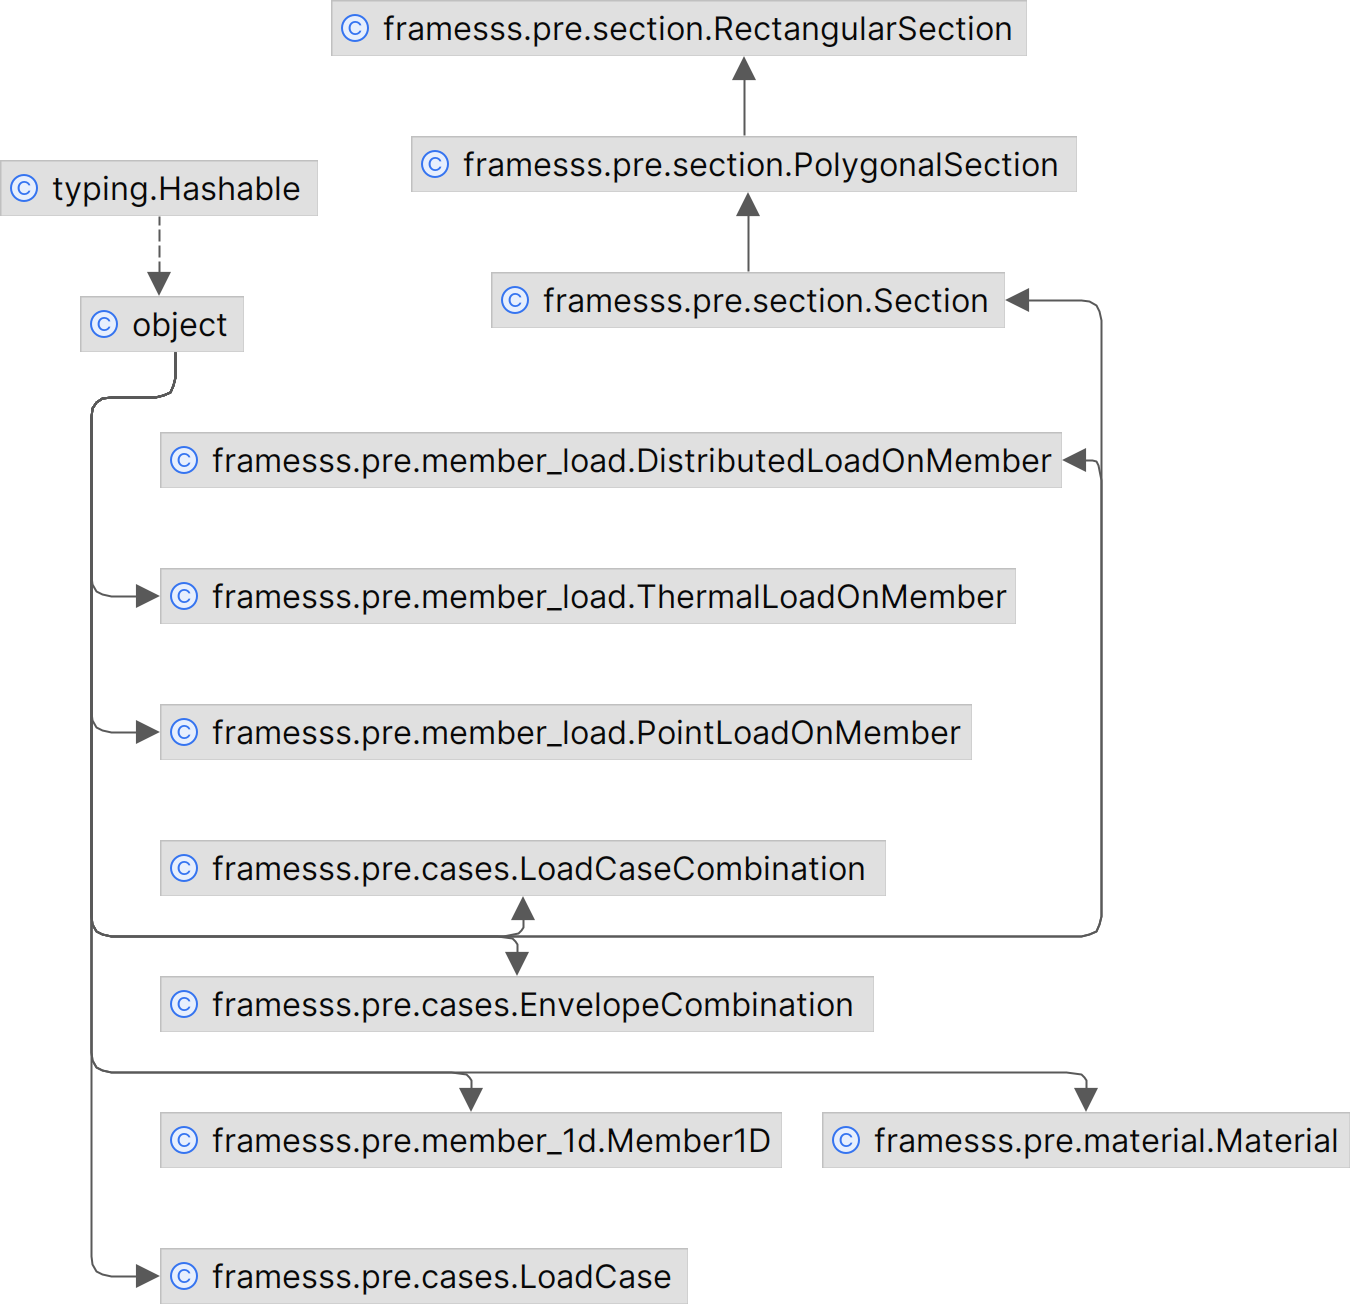
\includegraphics{assets/figures/framesss/uml/pre.png}
    \caption{Diagram modulu \texttt{pre}}
    \label{fig:modul_pre}
\end{figure}

%%%%%%%%%%%%%%%%%%%%%%%%%%%%%%%%%%%%%%%% FEA %%%%%%%%%%%%%%%%%%%%%%%%%%%%%%%%%%%%%%%%%%%%%%%

\subsubsection*{Modul \texttt{fea}}
Na obr. \ref{fig:modul_fea} je diagram zobrazující hierarchii tříd v~modulu 
\href{https://danberanek.github.io/framesss/gen/framesss.fea.html}{\texttt{fea}}, který je srdcem knihovny framesss. Klíčovou třídou je
\href{https://danberanek.github.io/framesss/gen/framesss.fea.models.model.Model.html#framesss.fea.models.model.Model}{\texttt{Model}}, která je zodpovědná za přidávání prvků (uzly, prvky, zatěžovací stavy, zatížení atd.) a drží v~sobě všechny instance, které se následně předávají do řešiče (solveru). Pod ní jsou specifické modely, jako
\href{https://danberanek.github.io/framesss/gen/framesss.fea.models.frame_xz.FrameXZModel.html#framesss.fea.models.frame_xz.FrameXZModel}{\texttt{FrameXZModel}}. Modul také obsahuje třídy pro definici elementů
\href{https://danberanek.github.io/framesss/gen/framesss.fea.element_1d.Element1D.html#framesss.fea.element_1d.Element1D}{\texttt{Element1D}}
 a uzlů
 \href{https://danberanek.github.io/framesss/gen/framesss.fea.node.Node.html#framesss.fea.node.Node}{ \texttt{Node}}. Pro zatížení elementů zde máme abstraktní třídu 
 \href{https://danberanek.github.io/framesss/gen/framesss.fea.boundary_conditions.element_load.ElementLoad.html#framesss.fea.boundary_conditions.element_load.ElementLoad}{\texttt{ElementLoad}}, ze které vychází třída pro zatížení spojitým zatížením
 \href{https://danberanek.github.io/framesss/gen/framesss.fea.boundary_conditions.element_load.DistributedLoad.html}{\texttt{DistributedLoad}}
 a třída pro zatížení teplotou
 \href{https://danberanek.github.io/framesss/gen/framesss.fea.boundary_conditions.element_load.ThermalLoad.html}{\texttt{ThermalLoad}}, dále je zde třída pro uzlové zatížení
 \href{https://danberanek.github.io/framesss/gen/framesss.fea.boundary_conditions.nodal_load.NodalLoad.html}{\texttt{NodalLoad}}, a pro předepsané přemístění podpor
\href{https://danberanek.github.io/framesss/gen/framesss.fea.boundary_conditions.prescribed_displacement.PrescribedDisplacement.html#framesss.fea.boundary_conditions.prescribed_displacement.PrescribedDisplacement}{ \texttt{PrescribedDisplacement}}.
 Modul také zahrnuje třídy pro specifikování dimenze problému, které vychází z~abstraktní třídy
 \href{https://danberanek.github.io/framesss/gen/framesss.fea.analysis.analysis.Analysis.html#framesss.fea.analysis.analysis.Analysis}{\texttt{Analysis}}
 a její konkrétní implementace pro různé typy konstrukcí, např.
 \href{https://danberanek.github.io/framesss/gen/framesss.fea.analysis.frame_xz_analysis.FrameXZAnalysis.html#framesss.fea.analysis.frame_xz_analysis.FrameXZAnalysis}{\texttt{FrameXZAnalysis}}.

\begin{figure}[H]
    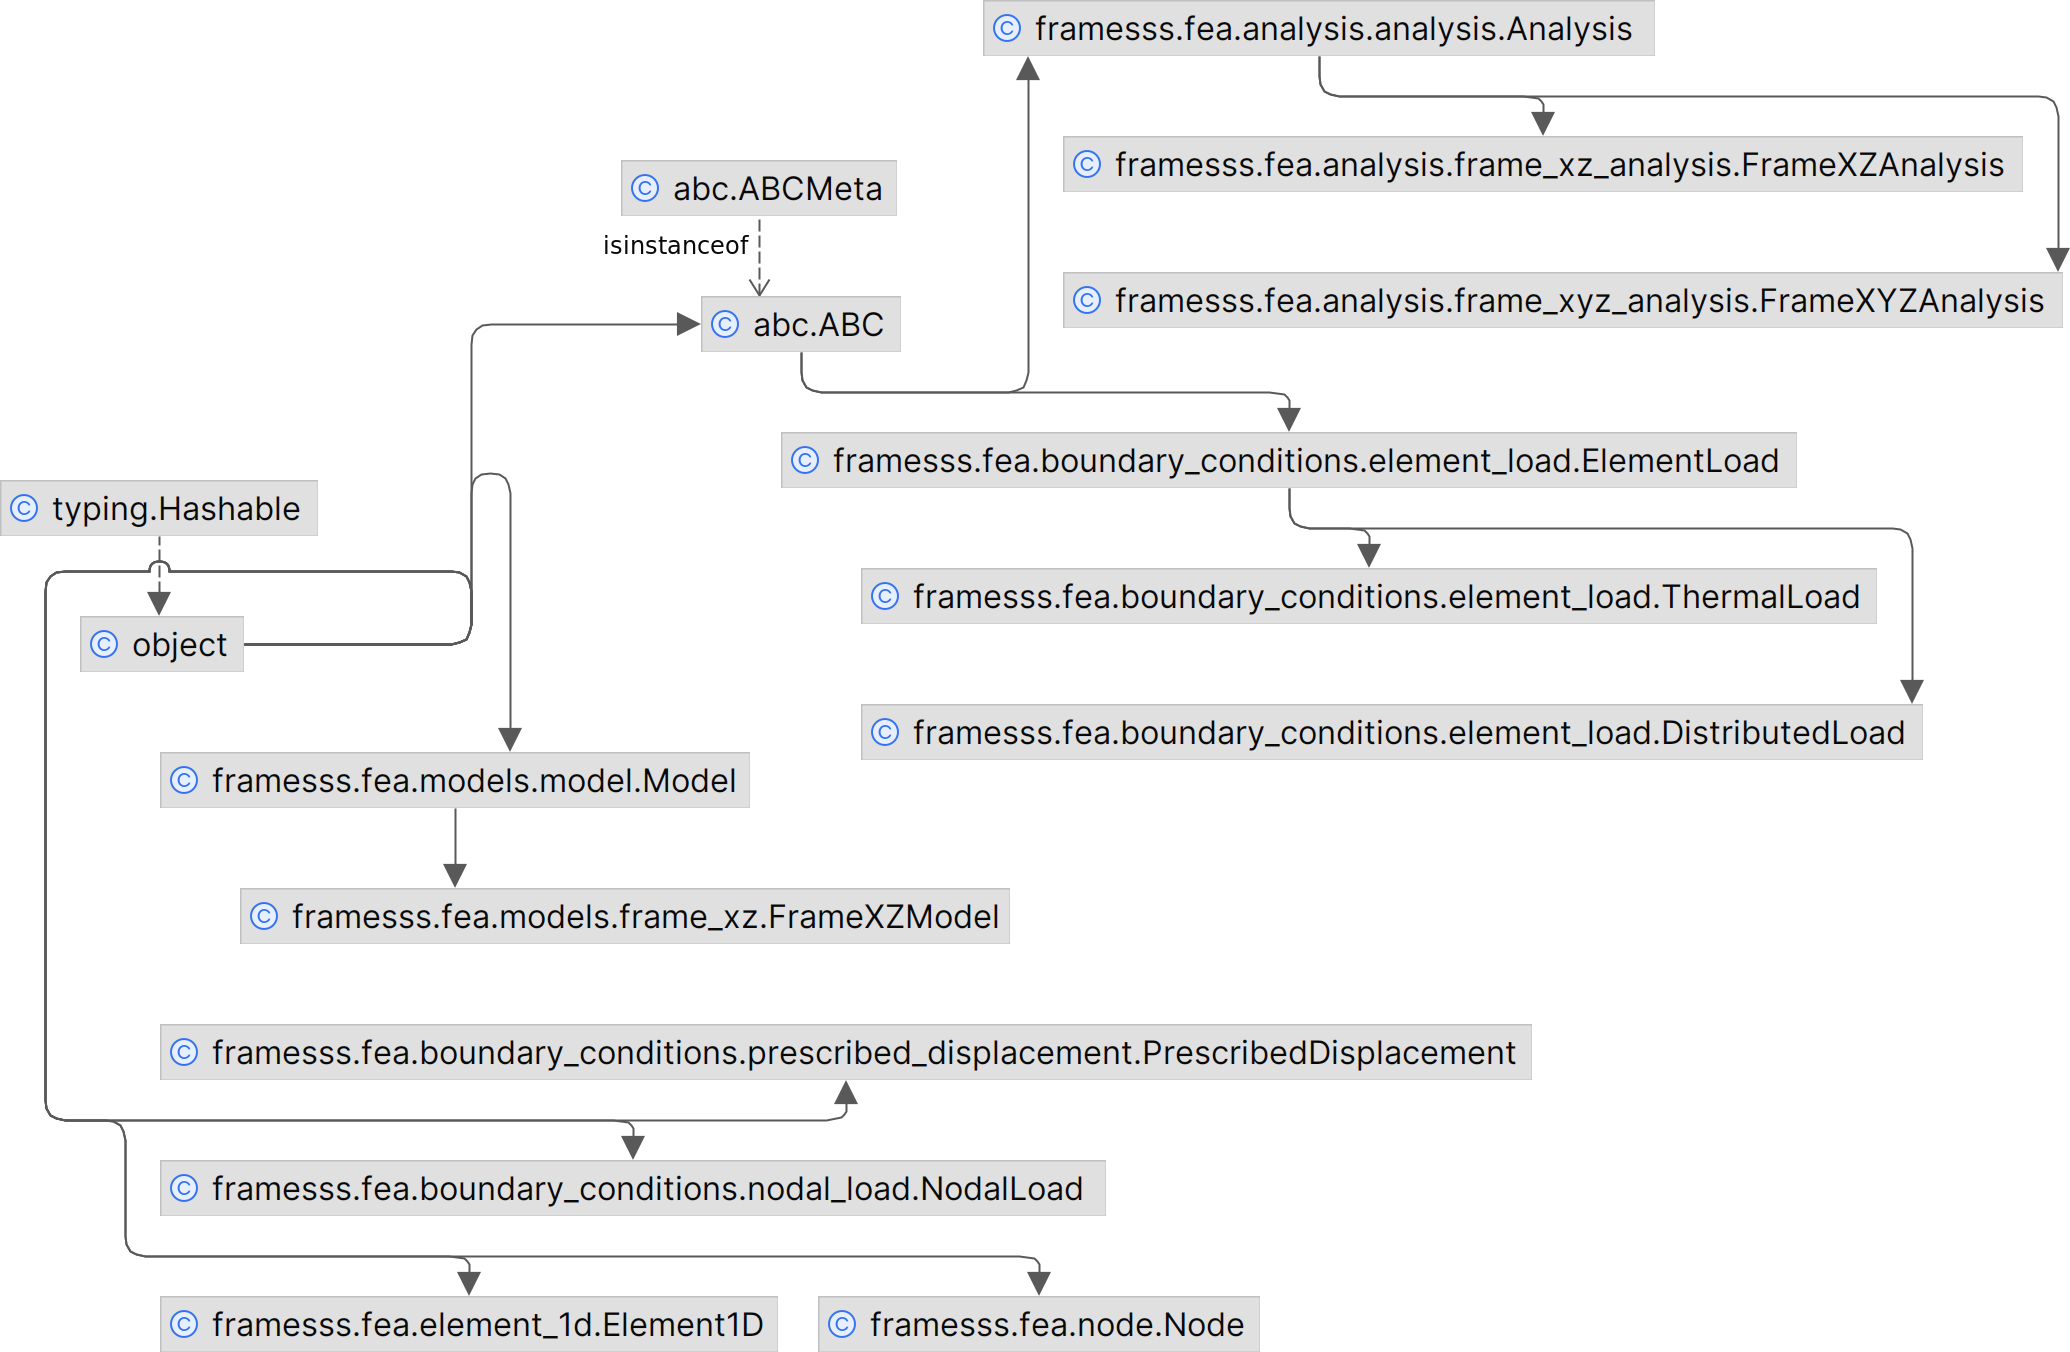
\includegraphics{assets/figures/framesss/uml/fea.png}
    \caption{Diagram modulu \texttt{fea}}
    \label{fig:modul_fea}
\end{figure}

\subsubsection*{Modul \texttt{solvers}}
Modul obsahuje řešiče používané pro výpočty v~modulu
\href{https://danberanek.github.io/framesss/gen/framesss.fea.html}{\texttt{fea}}. Na  obr. \ref{fig:modul_solvers} je znázorněný diagram hierarchie tříd v~modulu
\href{https://danberanek.github.io/framesss/gen/framesss.solvers.html}{\texttt{solvers}}. Základem této hierarchie je třída \texttt{abc.ABC}, což je základní abstraktní třída v~Pythonu. Na jejím základě je definována třída
\href{https://danberanek.github.io/framesss/gen/framesss.solvers.solver.Solver.html}{\texttt{Solver}}, která slouží jako základ pro konkrétní implementace řešičů. Jediným implementovaným řešičem je v~současné době třída
\href{https://danberanek.github.io/framesss/gen/framesss.solvers.linear_static.LinearStaticSolver.html}{\texttt{LinearStaticSolver}}, která implementuje lineární statické výpočty.

\begin{figure}[H]
    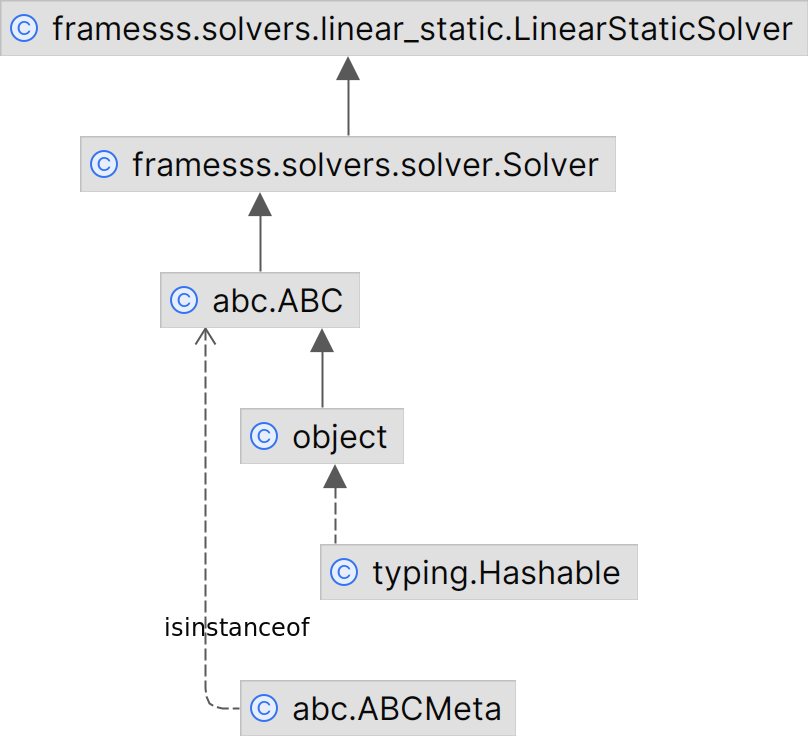
\includegraphics{assets/figures/framesss/uml/solvers.png}
    \caption{Diagram modulu \texttt{solvers}}
    \label{fig:modul_solvers}
\end{figure}

\subsubsection*{Modul \texttt{post}}
Zpracovává výsledky, jako jsou posuny a vnitřní síly, které jsou získány z~výpočtu provedených modulem \href{https://danberanek.github.io/framesss/gen/framesss.fea.html}{\texttt{fea}}. Modul nezahrnuje vizualizaci, ale umožňuje uživatelům extrahovat a prohlížet vypočítané hodnoty, které mohou být dále použity.
Diagram na obr. \ref{fig:modul_post} ukazuje hierarchii tříd v~modulu \href{https://danberanek.github.io/framesss/gen/framesss.post.html}{\texttt{post}}, který je zodpovědný za zpracování výsledků. Třída 
\href{https://danberanek.github.io/framesss/gen/framesss.post.member_1d_results.Member1DResults.html#framesss.post.member_1d_results.Member1DResults}{\texttt{Member1DResults}} zpracovává výsledky pro jednotlivé prutové prvky, třída
\href{https://danberanek.github.io/framesss/gen/framesss.post.node_results.NodeResults.html}{\texttt{NodeResults}} zpracovává výsledky pro jednotlivé uzly konstrukce.
\begin{figure}[H]
    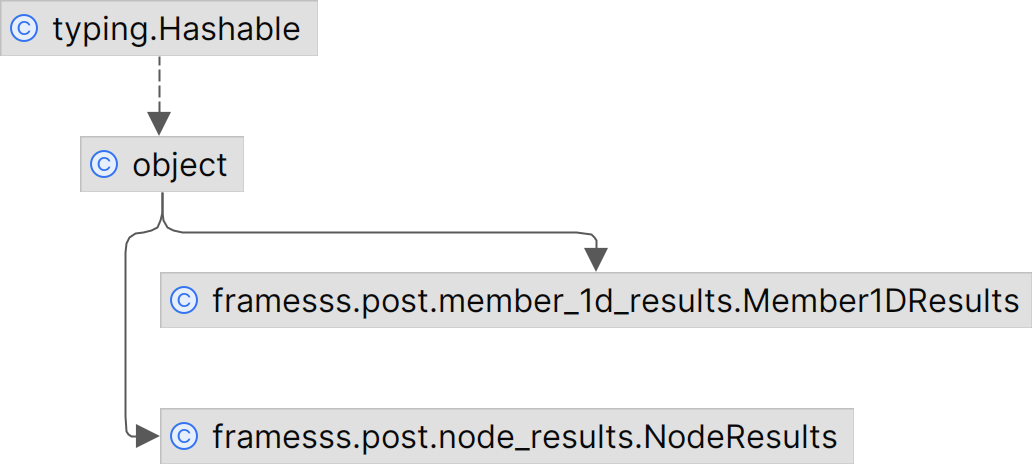
\includegraphics{assets/figures/framesss/uml/post.png}
    \caption{Diagram modulu \texttt{post}}
    \label{fig:modul_post}
\end{figure}

\subsection{Předpoklady}

V této sekci jsou uvedeny základní předpoklady, které byly přijaty při vývoji knihovny \texttt{framesss},
\begin{itemize}
    \item konstrukce je umístěna v pravotočivé souřadné soustavě,
    \item pro kladný směr pootočení platí pravidlo pravé ruky\footnote{Palec natočíme ve směru kladné části osy a zahnuté prsty pravé ruky značí kladný směr otáčení.},
    \item výpočet probíhá podle teorie malých deformací,
    \item materiál je uvažován jako pružný, platí Hookův zákon.
\end{itemize}

Tyto předpoklady umožňují uplatnění principu superpozice.

\subsubsection*{Předpoklady pro model v rovině XZ}

\begin{itemize}
    \item zatížení působí pouze v rovině \gls{X}\gls{Z}, která je zároveň rovinou symetrie,
    \item každý uzel má přiřazené tři stupně volnosti, posun ve směru globální osy \gls{X}, pootočení okolo globální osy \gls{Y} a posun ve směru globální osy \gls{Z}. Kladný směr je naznačený na \autoref{fig:global_dofs},    
    \begin{figure}[H]
        \input{assets/figures/framesss/global_dofs}
        \caption{Stupně volnosti v globálním systému}
        \label{fig:global_dofs}
    \end{figure}

    \item stupně volnosti a jejich kódová čísla\footnote{Indexování v jazyce Python začíná od $0$, což znamená, že první stupeň volnosti má přiřazené kódové číslo $0$, druhý prvek má kódové číslo $1$ atd.} v lokálním systému prutového prvku jsou označena na \autoref{fig:dof_numbering},
    
    \begin{figure}[H]
        \input{assets/figures/framesss/element_fef_dofs}
        \caption{Stupně volnosti v lokálním systému prvku}
        \label{fig:dof_numbering}
    \end{figure}

    \item vnitřní síly v jakémkoliv průřezu prvku jsou: normálová síla \gls{axial_force}, posouvající síla \gls{shear_force} a ohybový moment \gls{bending_moment}. Kladná orientace vnitřních sil je naznačená na \autoref{fig:positive_internal_forces}.
    \begin{figure}[H]
        \input{assets/figures/framesss/positive_internal_forces}
        \caption{Kladná orientace vnitřních sil}
        \label{fig:positive_internal_forces}
    \end{figure}
\end{itemize}


\subsection{Algoritmizace}

V~této sekci je představen algoritmus, který je jádrem metody konečných prvků implementované v~knihovně framesss. Tento algoritmus systematicky zpracovává model od jeho diskretizace až po výpočet odezvy konstrukce na zatížení jednotlivými zatěžovacími stavy a jejich kombinacemi.

\begin{algorithm}[H]
    \caption{Proces výpočtu modelu}
    \DontPrintSemicolon  % Don't print semicolons
    
    \SetKwFunction{FMain}{solve()}
    \SetKwProg{Fn}{Metoda}{:}{}
    \Fn{\FMain}{
        Diskretizace prutů na jednotlivé elementy\;
        Očíslování stupňů volnosti\;
        Lokalizace globální matice tuhosti\;
        \For{každý zatěžovací stav}{
            Inicializace vektoru koncových posunů\;
            Lokalizace předepsaných deformací\;
            Inicializace vektoru zatížení\;
            Lokalizace sil v~uzlech\;
            Lokalizace koncových sil na prvcích\; 
            Výpočet vektoru neznámých koncových posunů\;
            Výpočet reakcí\;
            Výpočet koeficientů vnitřních sil\;
            Výpočet extrémů vnitřních sil\;
            Uložení vypočítaných hodnot\;
        }
        \For{každá kombinace zatížení}{
            Inicializace výsledků\;
            \For{každý zatěžovací stav v~kombinaci}{
                Přičtení hodnot k~výsledkům\;
            }
            Uložení výsledků\;
        }
        \For{každá obálka}{
            Inicializace\;
            Určení extrémních hodnot v~každé kombinaci\;
            Uložení hodnot\;
        }
        \Return{}
    }
    
\end{algorithm}

\input{chapters/framesss/implementation/sparse.tex}

\subsection{Testování}

Pro zajištění spolehlivosti a přesnosti knihovny \texttt{framesss} byla implementována řada automatizovaných testů. Automatizované testování umožňuje včasné odhalení a opravu chyb, což přispívá k celkové stabilitě a kvalitě knihovny.

Testování knihovny \texttt{framesss} probíhá v různých verzích Pythonu (3.9, 3.10, 3.11, 3.12), aby byla odhalena případná kolize v závislostech mezi verzemi. Lokálně jsou testy spouštěny pomocí nástroje \texttt{nox} \cite{nox}, který vytváří virtuální prostředí, instaluje potřebné knihovny a spouští všechny testy, včetně validačních, \texttt{pre-commit} \cite{precommit} a \texttt{mypy} \cite{mypy} testů.

\subsubsection*{Unit testy}
Unit test je základní typ testu používaný v softwarovém vývoji, jehož cílem je ověřit správnou funkci jednotlivých částí kódu. Unit testy se zaměřují na testování nejmenších, izolovaných částí aplikace, jako jsou jednotlivé funkce nebo metody tříd. Hlavní charakteristiky unit testů jsou
\begin{itemize}
    \item \textbf{Izolace}: Testy jsou navrženy tak, aby byly nezávislé na ostatních částech kódu. Každý test kontroluje pouze jednu konkrétní část funkčnosti.
    \item \textbf{Automatizace}: Testy jsou spouštěny automaticky, což umožňuje rychlou a efektivní kontrolu správnosti
    \item \textbf{Opakovatelnost}: Testy mohou být opakovaně spouštěny při každé změně kódu, což zajišťuje, že nové změny neovlivní existující funkčnost.
\end{itemize}

\subsubsection*{Validační testy}
Kromě unit testů se správnost knihovny testuje na jednoduchých konstrukcích (prostý nosník, šikmé nosníky, konzoly, oboustranně vetknutý nosník apd.), kde je známé analytické řešení.

Pro validační testy byly použity následující zdroje:
\begin{itemize}
    \item \textit{DESIGN AID No. 6 — BEAM DESIGN FORMULAR WITH SHEAR AND MOMENT DIAGRAMS} od American Wood Council \cite{design_aid},
    \item \textit{Sbírka příkladů stavební mechaniky: princip virtuálních sil, silová metoda, deformační metoda} od Jíra, A. a kol. \cite{sbirka_prikladu}.
\end{itemize}

\subsubsection*{Kontinuální integrace a spuštění testů na GitHubu}
Kromě lokálního testování je nezbytné zajistit, aby všechny změny v kódu byly automaticky testovány i při jejich nahrání do centrálního repozitáře. Tento proces, známý jako kontinuální integrace (Continuous Integration, CI), je implementován pomocí GitHub Actions.

Při každém pushnutí změn do GitHub repozitáře se automaticky spustí CI pipeline, která zahrnuje následující kroky:
\begin{itemize}
    \item \textbf{Instalace závislostí}: Nezbytné knihovny a závislosti jsou nainstalovány podle specifikací v konfiguračním souboru.
    \item \textbf{Statická analýza kódu}: Kód je zkontrolován nástrojem mypy \cite{mypy}, který provádí statickou typovou kontrolu, aby se zajistila konzistence typů a odhalily potenciální typové chyby.
    \item \textbf{Spuštění unit testů}: Pomocí nástroje pytest \cite{pytest} se spustí všechny unit testy a validační testy, aby se ověřila funkčnost všech částí kódu.
\end{itemize}

Jednou z výhod používání GitHub Actions je možnost testovat kód na různých operačních systémech, knihovna \texttt{framesss} je testován na následujících platformách
\begin{itemize}
    \item \textbf{Windows},
    \item \textbf{Linux},
    \item \textbf{MacOS}.
\end{itemize}

\subsection{Příklad}

Následující příklad je převzat ze \textit{Sbírky příkladů stavební mechaniky} \cite[Příklad 5.2]{sbirka_prikladu}.

\begin{figure}[H]
    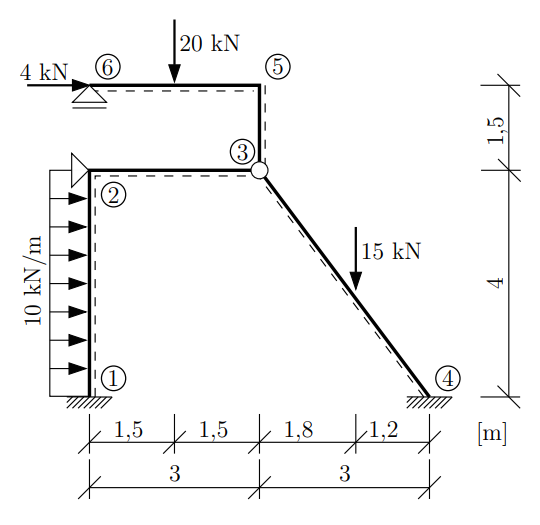
\includegraphics[height=7cm]{assets/figures/framesss/example_snk.png}
    \caption[Statické schéma konstrukce]{Statické schéma konstrukce, převzato z \cite[Příklad 5.2]{sbirka_prikladu}}
    \label{fig:framesss_example}
\end{figure}

Všechny pruty mají Youngův modul pružnosti $\gls{E} = \SI{30}{\GPa}$, moment setrvačnosti k ose, kolem které jsou pruty namáhané ohybem $\gls{I_y} = \SI{1e-3}{\unit{\metre\tothe{4}}}$ a plochu $\gls{A}= \SI{4e-3}{{\metre\tothe{2}}}$.

Na příkladu bude ilustrováno použití knihovny \texttt{framesss} v prostředí JupyterLab.

\input{chapters/framesss/implementation/example_jupyter_nb.tex}

\begin{table}[H]
    \setlength{\tabcolsep}{10pt}
    \renewcommand{\arraystretch}{1.2}
    \rowcolors{2}{ctulightblue!20}{white}
    \begin{tabular}{ccrrr}
        \rowcolor{ctulightblue} \bfseries veličina & \bfseries rozměr & \bfseries LC1 & \bfseries CO1 & \bfseries Sbírka \\ 
            $R_{1,\gls{x}}$ & $\SI{}{\kilo\newton}$ & -20.781 & -20.781 & -20.781 \\
            $R_{1,\gls{z}}$ & $\SI{}{\kilo\newton}$ &   0.000 &   0.000 &   0.000 \\
            \rowcolor{yellow!15}$M_{1,\gls{y}}$ & $\SI{}{\kilo\newton\metre}$ & -14.375 & -14.375 &  14.375 \\
            $R_{2,\gls{x}}$ & $\SI{}{\kilo\newton}$ & -15.258 & -15.258 & -15.258 \\
            \rowcolor{yellow!15}$R_{2,\gls{z}}$ & $\SI{}{\kilo\newton}$ &   3.750 &   3.750 &   -3.750 \\
            $R_{4,\gls{x}}$ & $\SI{}{\kilo\newton}$ &  -7.961 &  -7.961 &  -7.961 \\
            \rowcolor{yellow!15}$R_{4,\gls{z}}$ & $\SI{}{\kilo\newton}$ &  23.250 &  23.250 &  -23.249 \\
            \rowcolor{yellow!15}$M_{4,\gls{y}}$ & $\SI{}{\kilo\newton}$ &  10.905 &  10.905 &  -10.906 \\
            \rowcolor{yellow!15}$R_{6,\gls{z}}$ & $\SI{}{\kilo\newton}$ &   8.000 &   8.000 &  -8.000 \\
            $\gls{phi_i}[2]$ & $\SI{}{\radian}\cdot 10^{-5}$ & -6.942 & -6.942 & 6.942 \\
            \rowcolor{red!8}$\gls{u_i}[3]$ & $\SI{}{\metre}\cdot 10^{-5}$ & -9.902 & -9.902 & -9.903 \\
            \rowcolor{yellow!15}$\gls{w_i}[3]$ & $\SI{}{\metre}\cdot 10^{-4}$ & -9.168 & -9.168 & 9.168 \\
            $\gls{axial_force}_{1,2}$ & $\SI{}{\kilo\newton}$ & 0.000 & 0.000 & 0.000 \\
            %
            $\gls{axial_force}_{2,3}$ & $\SI{}{\kilo\newton}$ & -3.961 & -3.961 & -3.961 \\
            %
            $\min(\gls{axial_force}_{3,4})$ & $\SI{}{\kilo\newton}$ & -23.376 & -23.376 & -23.376 \\
            $\max(\gls{axial_force}_{3,4})$ & $\SI{}{\kilo\newton}$ & -11.376 & -11.376 & -11.376 \\
            %
            $\gls{axial_force}_{3,5}$ & $\SI{}{\kilo\newton}$ & -12.000 & -12.000 & -12.000 \\
            %
            $\gls{axial_force}_{6,5}$ & $\SI{}{\kilo\newton}$ & -4.000 & -4.000 & -4.000 \\
            %%%%%%%%%%%%%%%%%%%%%%%%%%%%%%%%%%%%%%%%%%%%%%%%%%%%%%%%%%%%%%%%%%%%%%%%%%%%%%%%%%%%%%%%%%
            $\min(\gls{shear_force}_{1,2})$ & $\SI{}{\kilo\newton}$ & -19.219 & -19.219 & -19.219 \\
            $\max(\gls{shear_force}_{1,2})$ & $\SI{}{\kilo\newton}$ & 20.781 & 20.781 & 20.781 \\
            %
            $\gls{shear_force}_{2,3}$ & $\SI{}{\kilo\newton}$ & 3.750 & 3.750 & 3.750 \\
            %
            $\min(\gls{shear_force}_{3,4})$ & $\SI{}{\kilo\newton}$ & -7.581 & -7.581 & -7.581 \\
            $\max(\gls{shear_force}_{3,4})$ & $\SI{}{\kilo\newton}$ & 1.419 & 1.419 & 1.419 \\
            %
            $\gls{shear_force}_{3,5}$ & $\SI{}{\kilo\newton}$ & 4.000 & 4.000 & 4.000 \\
            %
            $\min(\gls{shear_force}_{6,5})$ & $\SI{}{\kilo\newton}$ & -12.000 & -12.000 & -12.000 \\
            $\max(\gls{shear_force}_{6,5})$ & $\SI{}{\kilo\newton}$ & 8.000 & 8.000 & 8.000 \\
            %%%%%%%%%%%%%%%%%%%%%%%%%%%%%%%%%%%%%%%%%%%%%%%%%%%%%%%%%%%%%%%%%%%%%%%%%%%%%%%%%%%%%%%%%%
            $\min(\gls{bending_moment}_{1,2})$ & $\SI{}{\kilo\newton\meter}$ & -14.375 & -14.375 & -14.375 \\
            \rowcolor{red!8}$\max(\gls{bending_moment}_{1,2})$ & $\SI{}{\kilo\newton\meter}$ & 7.218 & 7.218 & 7.217 \\
            %
            $\min(\gls{bending_moment}_{2,3})$ & $\SI{}{\kilo\newton\meter}$ & -11.251 & -11.251 & -11.251 \\
            $\max(\gls{bending_moment}_{2,3})$ & $\SI{}{\kilo\newton\meter}$ & 0.000 & 0.000 & 0.000 \\
            %
            \rowcolor{red!8}$\min(\gls{bending_moment}_{3,4})$ & $\SI{}{\kilo\newton\meter}$ & -10.905 & -10.905 & -10.906 \\
            $\max(\gls{bending_moment}_{3,4})$ & $\SI{}{\kilo\newton\meter}$ & 4.257 & 4.257 & 4.257 \\
            %
            $\min(\gls{bending_moment}_{3,5})$ & $\SI{}{\kilo\newton\meter}$ & 0.000 & 0.000 & 0.000 \\
            $\max(\gls{bending_moment}_{3,5})$ & $\SI{}{\kilo\newton\meter}$ & 6.000 & 6.000 & 6.000 \\
            %
            $\min(\gls{bending_moment}_{6,5})$ & $\SI{}{\kilo\newton\meter}$ & -6.000 & -6.000 & -6.000 \\
            $\max(\gls{bending_moment}_{6,5})$ & $\SI{}{\kilo\newton\meter}$ & 12.000 & 12.000 & 12.000 
    \end{tabular}
    \caption{Porovnání výsledků}
    \label{tab:example_values}
\end{table}

V \autoref{tab:example_values} jsou uvedeny hodnoty vypočítané knihovnou \texttt{framesss} a srovnány s referenčními hodnotami ze \textit{Sbírky příkladů stavební mechaniky} \cite{sbirka_prikladu}. Testování probíhalo ve dvou různých scénářích: zatěžovací stav (LC1) a kombinace zatěžovacích stavů (CO1). LC1 představuje stav, kde je veškeré zatížení aplikováno najednou. CO1 je kombinace jednotlivých zatěžovacích stavů, kde každé zatížení bylo odděleně definováno a hodnota zatížení byla vydělena předem definovaným součinitel. Následně byly tyto zatěžovací stavy zkombinovány do kombinace zatěžovacích stavů s těmito součiniteli.

Porovnání výsledků ukazuje, že hodnoty vypočítané knihovnou \texttt{framesss} jsou téměř stejné jako referenční hodnoty, přičemž rozdíly (vyznačené \colorbox{red!8}{červenou barvou}) se nacházejí v rámci zaokrouhlovací chyby.

Hodnoty posunutí a reakcí ve směru osy \gls{Z} a hodnoty pootočení a momentů okolo osy \gls{Y} vykazují opačné znaménko (vyznačeno \colorbox{yellow!15}{žlutou barvou}) ve srovnání s referenčními hodnotami, což je způsobeno rozdílným natočením globálního souřadného systému, viz obr. \ref{fig:example_coordinate_systems}. Systém ze sbírky je vlevo, uvažovaný systém při zadávání konstrukce v této práci vpravo. Při stanovení kladného směru pootočení platí pravidlo pravé ruky.

\begin{figure}[H]
    \input{assets/figures/framesss/example_coordinate_systems}
    \caption{Porovnání souřadných systémů}
    \label{fig:example_coordinate_systems}
\end{figure}



\chapter{Knihovna pro navrhování konstrukcí podle Eurokódů}

Knihovna desssign byla vyvinuta s~cílem usnadnit klasifikaci, třídění a generování zatěžovacích stavů podle požadavků Eurokódu. Eurokódy představují soubor evropských norem pro navrhování konstrukcí, které obsahují specifické požadavky na kombinace zatížení a jejich součinitele. Tato knihovna umožňuje automatizaci tohoto procesu.

Hlavním důvodem vzniku knihovny bylo zajistit, aby bylo možné automaticky generovat kombinace zatěžovacích stavů podle jejich charakteru a přiřazovat jednotlivým zatěžovacím stavům odpovídající součinitele, jak to vyžadují Eurokódy. Tento přístup umožňuje snadno a rychle vytvářet správné kombinace zatížení, které mohou být následně použity v~knihovně framesss pro statické výpočty prutových konstrukcí.

Při návrhu knihovny pro analýzu konstrukcí framesss jsem chtěl zachovat její obecnost a flexibilitu, aniž by byla zatížena specifickými normami nebo jinými specifickými závislostmi. Cílem bylo vytvořit obecný program pro analýzu prutových konstrukcí, který by nebyl příliš komplikovaný a nebyl závislý na konkrétní normě. Knihovna desssign tedy vznikla jako doplněk k~framesss, aby umožnila specifickou implementaci podle Eurokódů, aniž by zatěžovala základní knihovnu zbytečnými závislostmi.

Knihovna desssign se skládá z~několika modulů, z~nichž nejvýznamnější je modul \texttt{loads}. Tento modul obsahuje třídy a funkce potřebné pro definici a správu zatěžovacích stavů a jejich kombinací. Mezi hlavní třídy patří \texttt{DesignLoadCase}, \texttt{DesignLoadCaseCombination} a \texttt{DesignLoadCaseGroup}, které umožňují definici vztahů mezi jednotlivými zatěžovacími stavy. Dále je zde třída \texttt{CombinationsGenerator}, která generuje kombinace zatížení na základě zadaného mezního stavu, typu kombinace a klasifikaci zatěžovacích stavů.

Knihovna také obsahuje submodul pro generování zatížení sněhem a větrem pro jednoduché tvary střech.

V~následujících částech této kapitoly se podrobněji podíváme na architekturu knihovny desssign, jednotlivé moduly a jejich funkce, a také na praktické použití této knihovny v~kontextu navrhování konstrukcí podle Eurokódů.

Zdrojový kód desssign je veřejně dostupný na platformě GitHub na adrese \url{https://github.com/DanBeranek/desssign}. Dokumentace knihovny, která je k~dispozici na adrese \url{https://danberanek.github.io/desssign/index.html}, poskytuje podrobné informace o~funkcionalitě, implementaci a použití knihovny.

\section{Instalace}
Knihovna desssign je snadno instalovatelná pomocí pip. Pro instalaci knihovny desssign stačí spustit následující příkaz v~terminálu:

\begin{verbatim}
pip install desssign
\end{verbatim}

Podrobný návod na instalaci knihovny v~Python virtuálním prostředí lze nalézt v~\autoref{sec:framesss_instalation}.

\section{Architektura knihovny}
Knihovna desssign je navržena jako modulární a rozšiřitelný systém, který umožňuje snadnou integraci nových funkcionalit. Hlavní moduly knihovny zahrnují modul \texttt{loads} a modul \texttt{wood}. Tato část kapitoly se zaměří na popis struktury knihovny a jednotlivých modulů.

\subsection{Struktura knihovny}
Knihovna desssign je organizována do následujících hlavních modulů
\begin{itemize}
    \item \textbf{loads}: Tento modul obsahuje třídy a funkce pro definici, správu a generování kombinací zatěžovacích stavů. Hlavní třídy zahrnují \texttt{DesignLoadCase}, \texttt{DesignLoadCaseCombination}, \texttt{DesignLoadCaseGroup} a \texttt{CombinationsGenerator}. Tento modul také obsahuje submodul pro generování zatížení sněhem a větrem pro jednoduché tvary střech.
    \item \textbf{wood}: Tento modul obsahuje funkce pro posouzení dřevěných konstrukcí podle \textit{ČSN EN 1995-1-1}. Přestože se jedná o~důležitou součást knihovny, v~této diplomové práci se zaměříme především na modul \texttt{loads}.
\end{itemize}

\subsubsection*{Modul \texttt{loads}}
Modul \texttt{loads} je klíčovou součástí knihovny desssign a je zodpovědný za
\begin{itemize}
    \item \textbf{Definic zatěžovacích stavů}:  Pomocí tříd \texttt{DesignLoadCase} a \texttt{DesignLoadCaseCombination}, které dědí vlastnosti tříd z~knihovny framesss, lze definovat jednotlivé zatěžovací stavy a jejich kombinace.
    \item \textbf{Kategorizaci zatěžovacích stavů}: Třída \texttt{DesignLoadCaseGroup} umožňuje definovat vztahy mezi jednotlivými zatěžovacími stavy.
    \item \textbf{Generování kombinací zatížení}: Třída \texttt{CombinationsGenerator} umožňuje automatické generování kombinací zatížení na základě zadaných parametrů a kategorizaci zatěžovacích stavů.
\end{itemize}

Tento modul také zahrnuje submodul pro klimatická zatížení, který umožňuje generování hodnot zatížení sněhem na střeše podle kapitoly 5 v~ČSN EN 1991-1-3 \cite{EN1991_1_3} a zatížení větrem pro obdélníkový tvar střech podle kapitoly 5 v~ČSN EN 1991-1-4 \cite{EN1991_1_4}.

\begin{figure}[H]
    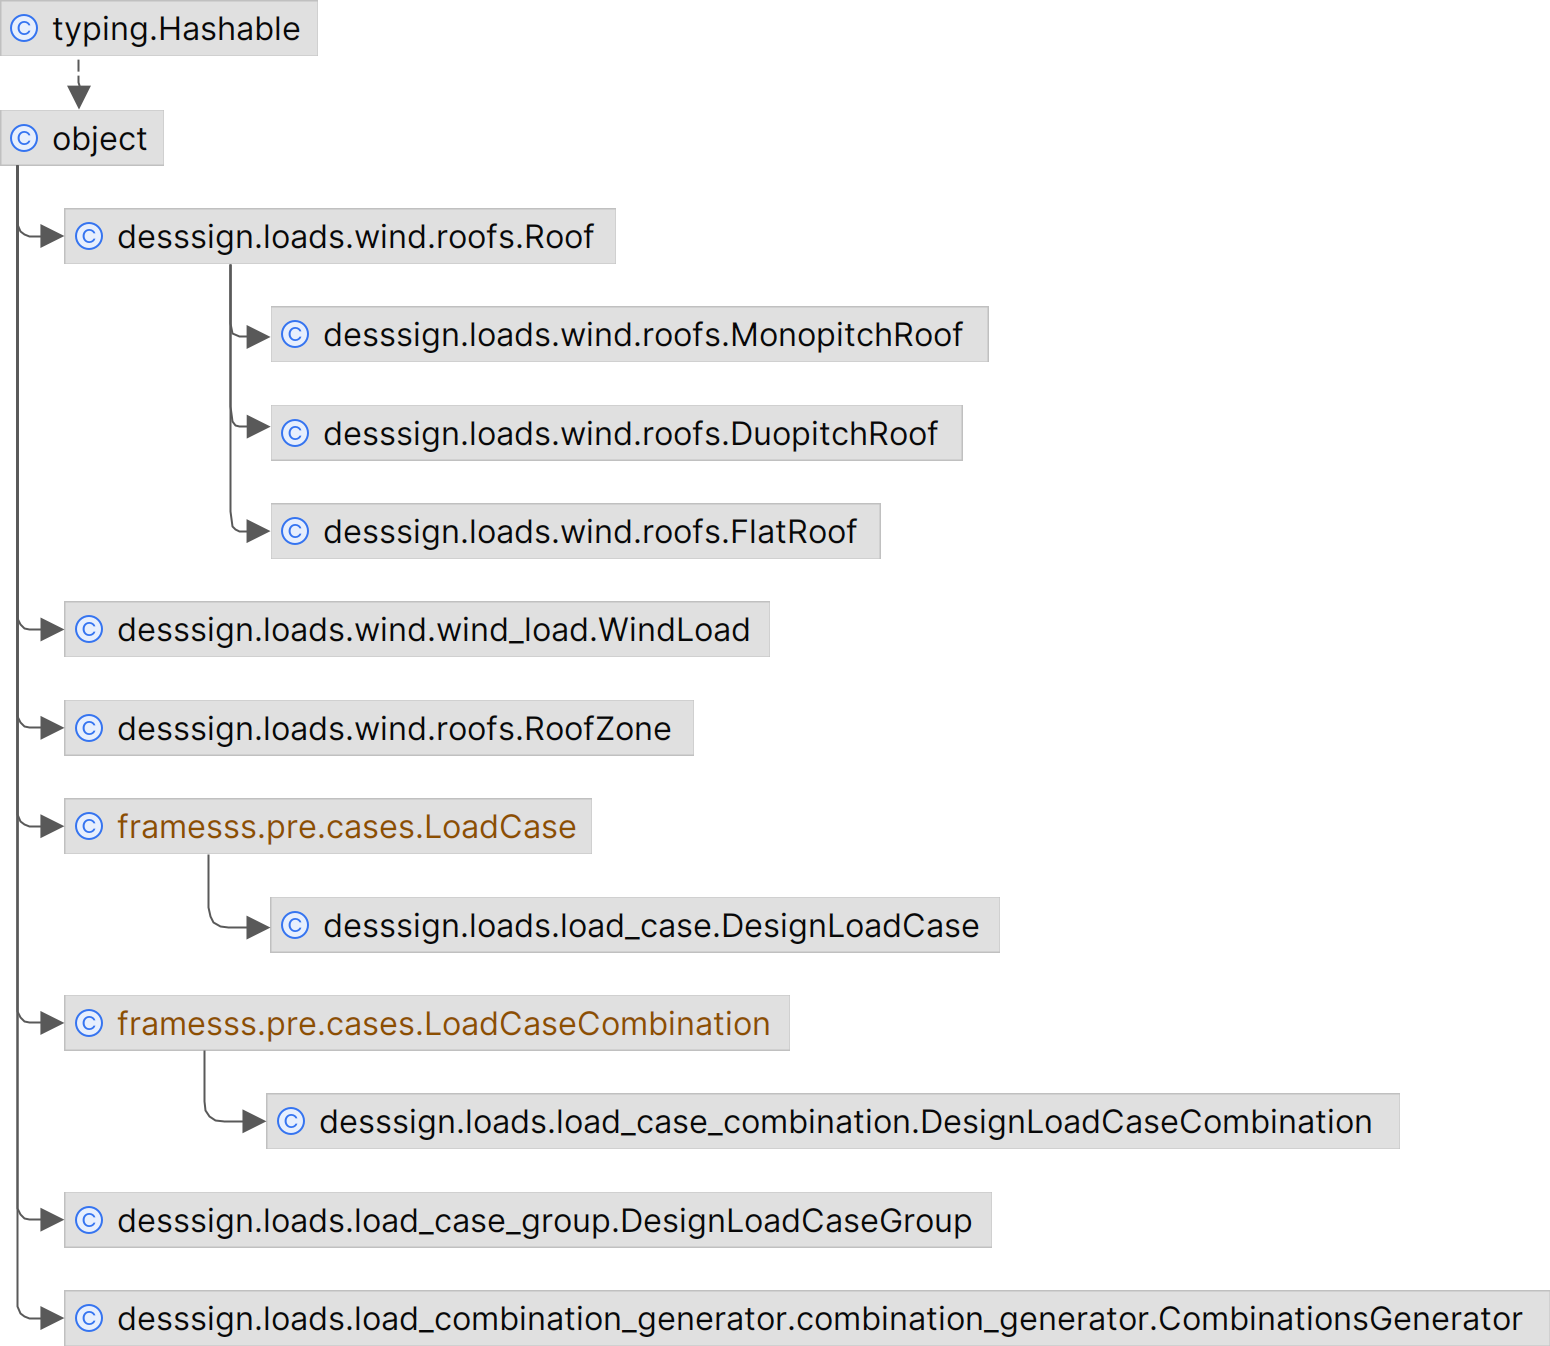
\includegraphics{assets/figures/desssign/loads_uml.png}
    \caption{Diagram modulu \texttt{loads}}
    \label{fig:modul_loads}
\end{figure}

\subsection{Integrace s~knihovnou pro výpočty prutových konstrukcí}
Jednou z~klíčových vlastností knihovny desssign je její schopnost generovat kombinace zatěžovacích stavů, které lze následně použít v~knihovně framesss pro statické výpočty. Tímto způsobem knihovna desssign výrazně usnadňuje a automatizuje proces návrhu konstrukcí podle Eurokódů.

\subsubsection*{Třída \texttt{DesignLoadCase}}
Tato třída rozšiřuje třídu \texttt{LoadCase} z~knihovny framesss a přidává specifické atributy, 
\begin{itemize}
    \item \texttt{load\_type}: typ zatížení, lze volit mezi stálým a užitným zatížením,
    \item \texttt{category}: kategorie zatížení podle ČSN EN 1991-1-1, kapitola 6.3.1.1 \cite{EN1991_1_1}, specifikuje se pouze pro užitné zatížení,
    \item \texttt{load\_duration\_class}: třída trvání zatížení podle ČSN EN 1995-1-1, tab. 2.1 \cite{EN1995_1_1}.
\end{itemize}

\begin{figure}[H]
    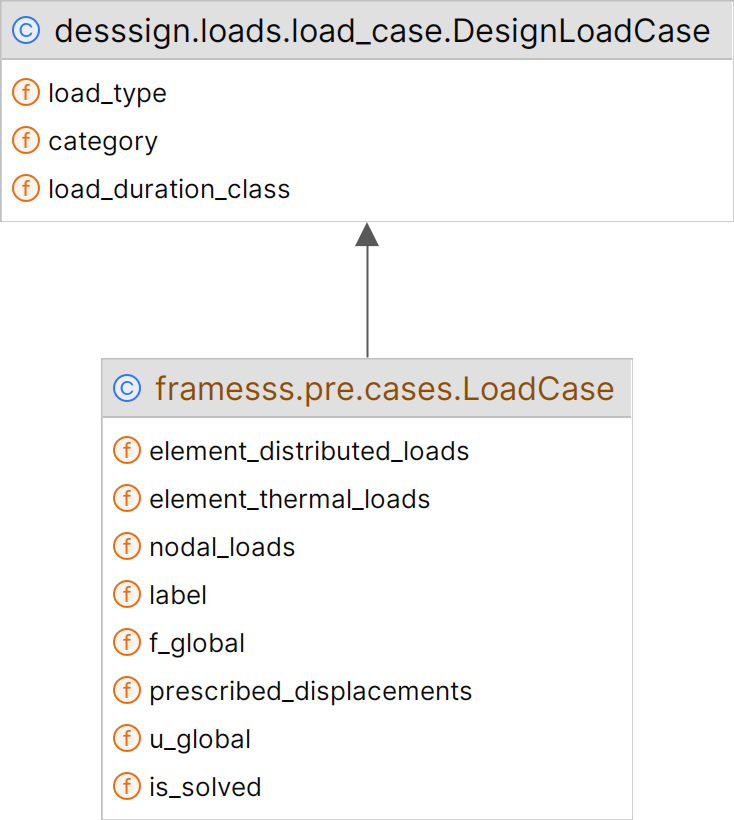
\includegraphics[height=8cm]{assets/figures/desssign/load_case.png}
    \caption{Diagram třídy \texttt{DesignLoadCase}}
    \label{fig:class_design_load_case}
\end{figure}

\subsubsection*{Třída \texttt{DesignLoadCaseCombination}}
Tato třída rozšiřuje třídu \texttt{LoadCaseCombination} z~knihovny framesss a zahrnuje atributy
\begin{itemize}
    \item \texttt{permanent\_cases}: zatěžovací stavy pro stálé zatížení,
    \item \texttt{leading\_variable\_case}: zatěžovací stav pro hlavní proměnné zatížení,
    \item \texttt{other\_variable\_cases}: vedlejší proměnné zatěžovací stavy,
    \item \texttt{limit\_state}: mezní stav,
    \item \texttt{combination\_type}: typ kombinace,
    \item \texttt{alternative\_combination}: specifikátor použité rovnice, vyžadovaný pouze pro alternativní kombinace MSÚ, buď \texttt{'6.10a'}, nebo \texttt{'6.10b'}, 
    \item \texttt{combination\_key}: automaticky vygenerovaný kombinační klíč.
\end{itemize}

Podle zadaného mezního stavu a kombinace se jednotlivým zatěžovacím automaticky přiřadí kombinační součinitelé podle pravidel v~ČSN EN 1990 \cite{EN1990}.

\begin{figure}[H]
    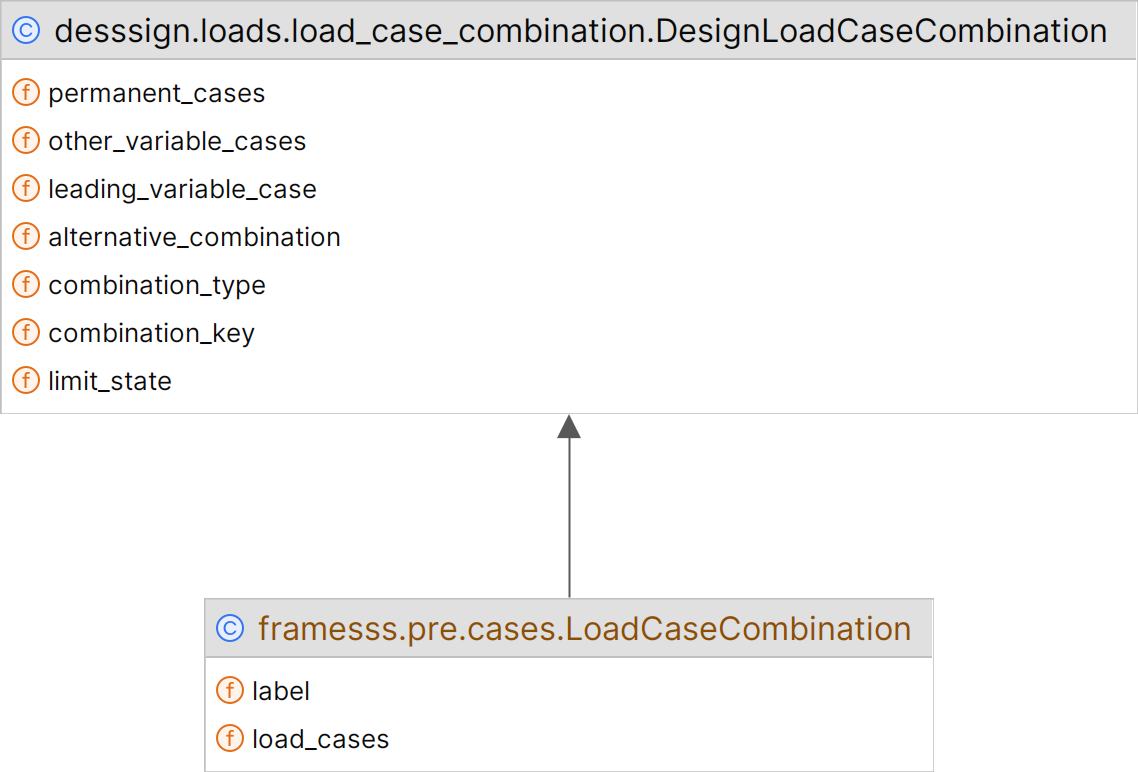
\includegraphics[height=8cm]{assets/figures/desssign/load_combinations.png}
    \caption{Diagram třídy \texttt{DesignLoadCaseComtination}}
    \label{fig:class_design_load_case_combination}
\end{figure}

\subsubsection*{Třída \texttt{DesignLoadCaseGroup}}
Třída \texttt{DesignLoadCaseGroup} umožňuje definovat vztahy mezi jednotlivými zatěžovacími stavy. Tato třída je klíčová pro správné generování kombinací zatěžovacích stavů.

Atributy:
\begin{itemize}
    \item \texttt{load\_case\_relation}: definuje vztah mezi zatěžovacími stavy,
    \begin{itemize}
        \item zatěžovací stavy působí vždy společně (např. stálá zatížení),
        \item zatěžovací stavy můžou a nemusí působit společně (např. užitná zatížení),
        \item zatížovací stavy nikdy nepůsobí společně.
    \end{itemize}
    \item \texttt{load\_cases}: zatěžovací stavy.
\end{itemize}

\begin{figure}[H]
    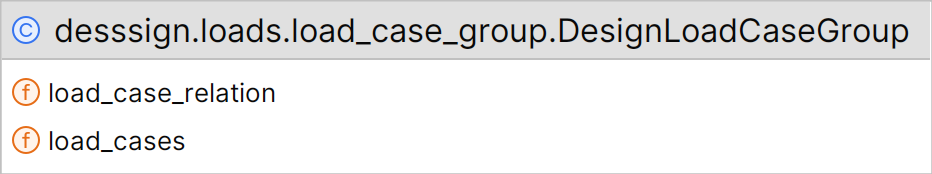
\includegraphics{assets/figures/desssign/design_load_case_group.png}
    \caption{Diagram třídy \texttt{DesignLoadCaseGroup}}
    \label{fig:class_design_load_case_group}
\end{figure}

\subsubsection*{Třída \texttt{CombinationsGenerator}}
Třída \texttt{CombinationsGenerator} je zodpovědná za generování kombinací zatížení na základě zadaného mezního stavu a typu kombinace.

Atributy:
\begin{itemize}
    \item \texttt{limit\_state}: typ mezního stavu (mezní stav únosnosti, mezni stav použitelnosti),
    \item \texttt{combination\_type}: typ kombinace zatížení (základní, alternativní, charakteristická, častá, kvazistálá)
\end{itemize}

Metody:
\begin{itemize}
    \item \texttt{generate\_combinations(load\_case\_groups)}: generuje kombinace zatížení na základě listu instancí \texttt{DesignLoadCaseGroup}.
\end{itemize}

Kombinace zatížení se generují podle vztahů uvedených v~kapitole 6 ČSN EN 1990 \cite{EN1990},
\begin{itemize}
    \item mezní stavy únosnosti, kombinace pro trvalé a dočasné návrhové situace:
        \begin{itemize}
            \item základní kombinace zatížení podle vztahu 6.10,
            \begin{equation}
                \sum_{j \geq 1} \gamma_{G,j} G_{k,j} "+" \gamma_P P "+" \gamma_{Q,1} Q_{k,1} "+" \sum_{i > 1} \gamma_{Q,i} \psi_{0,i} Q_{k,i},
            \end{equation}
            \item alternativní kombinace zatížení podle vztahu 6.10a a 6.10b,
            \begin{subequations}
                \begin{equation}
                    \sum_{j \geq 1} \gamma_{G,j} G_{k,j} "+" \gamma_P P "+" \gamma_{Q,1} \psi_{0,1} Q_{k,1} "+" \sum_{i > 1} \gamma_{Q,i} \psi_{0,i} Q_{k,i},
                \end{equation}
                \begin{equation}
                    \sum_{j \geq 1} \xi_j \gamma_{G,j} G_{k,j} "+" \gamma_P P "+" \gamma_{Q,1} Q_{k,1} "+" \sum_{i > 1} \gamma_{Q,i} \psi_{0,i} Q_{k,i},
                \end{equation}
            \end{subequations}
        \end{itemize}
    \item mezní stavy použitelnosti,
    \begin{itemize}
        \item charakteristická kombinace zatížení podle vztahu 6.14b,
            \begin{equation}
                \sum_{j \geq 1} G_{k,j} "+" P "+" Q_{k,1} "+" \sum_{i > 1} \psi_{0,i} Q_{k,i},
            \end{equation}
        \item častá kombinace zatížení podle vztahu 6.15b,
            \begin{equation}
                \sum_{j \geq 1} G_{k,j} "+" P "+" \psi_{1,i} Q_{k,1} "+" \sum_{i > 1} \psi_{2,i} Q_{k,i},
            \end{equation}
        \item kvazistálou kombinaci zatížení podle vztahu 6.16b,
            \begin{equation}
                \sum_{j \geq 1} G_{k,j} "+" \sum_{i \geq 1} \psi_{2,i} Q_{k,i},
            \end{equation}
    \end{itemize}
\end{itemize}
kde $G$ označuje stálé zatížení, $Q$ proměnné zatížení, $Q_{1}$ označuje hlavní proměnné zatížení, $\gamma$ jsou dílčí součinitelé zatížení podle ČSN EN 1990, příloha A~\cite{EN1990}, $\psi$ jsou součinitele pro proměnná zatížení podle ČSN EN 1990, příloha A~\cite{EN1990} a $\xi$ je redukční součinitel pro stálé zatížení.

\section{Příklad použití}

Pro klasifikaci zatěžovacích jsou v~knihovně vytvořeny \texttt{Enum}\footnote{\texttt{Enum} je speciální datový typ, který umožňuje definovat sadu pojmenovaných konstant.} třídy, které jasně stanovují způsob, jakým způsobem se mají zadávat parametry při vytváření nových instancí. Tyto \texttt{Enum} třídy zajišťují, že parametry jsou zadávány konzistentně a správně, což minimalizuje riziko chyb při definování zatěžovacích stavů.

Nejprve musíme do prostředí JupyterLab importovat všechny potřebné třídy a balíčky.
\begin{tcolorbox}[breakable, size=fbox, boxrule=1pt, pad at break*=1mm,colback=cellbackground, colframe=cellborder]
    \prompt{In}{incolor}{1}{\boxspacing}
    \begin{Verbatim}[commandchars=\\\{\}]
    \PY{k+kn}{from} \PY{n+nn}{desssign}\PY{n+nn}{.}\PY{n+nn}{loads}\PY{n+nn}{.}\PY{n+nn}{enums} \PY{k+kn}{import} \PY{n}{LoadType}
    \PY{k+kn}{from} \PY{n+nn}{desssign}\PY{n+nn}{.}\PY{n+nn}{loads}\PY{n+nn}{.}\PY{n+nn}{enums} \PY{k+kn}{import} \PY{n}{LimitState}
    \PY{k+kn}{from} \PY{n+nn}{desssign}\PY{n+nn}{.}\PY{n+nn}{loads}\PY{n+nn}{.}\PY{n+nn}{enums} \PY{k+kn}{import} \PY{n}{VariableCategory} \PY{k}{as} \PY{n}{cat}
    \PY{k+kn}{from} \PY{n+nn}{desssign}\PY{n+nn}{.}\PY{n+nn}{loads}\PY{n+nn}{.}\PY{n+nn}{enums} \PY{k+kn}{import} \PY{n}{ULSCombination} \PY{k}{as} \PY{n}{uls}
    \PY{k+kn}{from} \PY{n+nn}{desssign}\PY{n+nn}{.}\PY{n+nn}{loads}\PY{n+nn}{.}\PY{n+nn}{enums} \PY{k+kn}{import} \PY{n}{SLSCombination} \PY{k}{as} \PY{n}{sls}
    \PY{k+kn}{from} \PY{n+nn}{desssign}\PY{n+nn}{.}\PY{n+nn}{loads}\PY{n+nn}{.}\PY{n+nn}{enums} \PY{k+kn}{import} \PY{n}{ULSAlternativeCombination} \PY{k}{as} \PY{n}{alt}
    \PY{k+kn}{from} \PY{n+nn}{desssign}\PY{n+nn}{.}\PY{n+nn}{loads}\PY{n+nn}{.}\PY{n+nn}{enums} \PY{k+kn}{import} \PY{n}{LoadCaseRelation} \PY{k}{as} \PY{n}{rel}
    
    \PY{k+kn}{from} \PY{n+nn}{desssign}\PY{n+nn}{.}\PY{n+nn}{loads}\PY{n+nn}{.}\PY{n+nn}{load\PYZus{}case} \PY{k+kn}{import} \PY{n}{DesignLoadCase}
    \PY{k+kn}{from} \PY{n+nn}{desssign}\PY{n+nn}{.}\PY{n+nn}{loads}\PY{n+nn}{.}\PY{n+nn}{load\PYZus{}case\PYZus{}group} \PY{k+kn}{import} \PY{n}{DesignLoadCaseGroup}
    \PY{k+kn}{from} \PY{n+nn}{desssign}\PY{n+nn}{.}\PY{n+nn}{loads}\PY{n+nn}{.}\PY{n+nn}{load\PYZus{}combination\PYZus{}generator}\PY{n+nn}{.}\PY{n+nn}{combination\PYZus{}generator} \PY{k+kn}{import} \PY{n}{CombinationsGenerator}
    \end{Verbatim}
    \end{tcolorbox}

Vytvoříme 5 instancí typu \texttt{DesignLoadCase}, dva zatěžovací stavy pro stálé zatížení (\texttt{G1, G2}), jeden zatěžovací stav pro užitné zatížení kategorie A~(\texttt{Q3}) a dva zatěžovací stavy pro zatížení sněhem (\texttt{S4, S5}).
        \begin{tcolorbox}[breakable, size=fbox, boxrule=1pt, pad at break*=1mm,colback=cellbackground, colframe=cellborder]
    \prompt{In}{incolor}{2}{\boxspacing}
    \begin{Verbatim}[commandchars=\\\{\}]
    \PY{n}{G1} \PY{o}{=} \PY{n}{DesignLoadCase}\PY{p}{(}
        \PY{n}{label}\PY{o}{=}\PY{l+s+s2}{\PYZdq{}}\PY{l+s+s2}{G1}\PY{l+s+s2}{\PYZdq{}}\PY{p}{,}
        \PY{n}{load\PYZus{}type}\PY{o}{=}\PY{n}{LoadType}\PY{o}{.}\PY{n}{PERMANENT}\PY{p}{,}
    \PY{p}{)}
    
    \PY{n}{G2} \PY{o}{=} \PY{n}{DesignLoadCase}\PY{p}{(}
        \PY{n}{label}\PY{o}{=}\PY{l+s+s2}{\PYZdq{}}\PY{l+s+s2}{G2}\PY{l+s+s2}{\PYZdq{}}\PY{p}{,}
        \PY{n}{load\PYZus{}type}\PY{o}{=}\PY{n}{LoadType}\PY{o}{.}\PY{n}{PERMANENT}\PY{p}{,}
    \PY{p}{)}
    
    \PY{n}{Q3} \PY{o}{=} \PY{n}{DesignLoadCase}\PY{p}{(}
        \PY{n}{label}\PY{o}{=}\PY{l+s+s2}{\PYZdq{}}\PY{l+s+s2}{Q3}\PY{l+s+s2}{\PYZdq{}}\PY{p}{,}
        \PY{n}{load\PYZus{}type}\PY{o}{=}\PY{n}{LoadType}\PY{o}{.}\PY{n}{VARIABLE}\PY{p}{,}
        \PY{n}{category}\PY{o}{=}\PY{n}{cat}\PY{o}{.}\PY{n}{A}\PY{p}{,}
    \PY{p}{)}
    
    \PY{n}{S4} \PY{o}{=} \PY{n}{DesignLoadCase}\PY{p}{(}
        \PY{n}{label}\PY{o}{=}\PY{l+s+s2}{\PYZdq{}}\PY{l+s+s2}{S4}\PY{l+s+s2}{\PYZdq{}}\PY{p}{,}
        \PY{n}{load\PYZus{}type}\PY{o}{=}\PY{n}{LoadType}\PY{o}{.}\PY{n}{VARIABLE}\PY{p}{,}
        \PY{n}{category}\PY{o}{=}\PY{n}{cat}\PY{o}{.}\PY{n}{SNOW\PYZus{}BELLOW\PYZus{}1000\PYZus{}M}\PY{p}{,}
    \PY{p}{)}
    
    
    \PY{n}{S5} \PY{o}{=} \PY{n}{DesignLoadCase}\PY{p}{(}
        \PY{n}{label}\PY{o}{=}\PY{l+s+s2}{\PYZdq{}}\PY{l+s+s2}{S5}\PY{l+s+s2}{\PYZdq{}}\PY{p}{,}
        \PY{n}{load\PYZus{}type}\PY{o}{=}\PY{n}{LoadType}\PY{o}{.}\PY{n}{VARIABLE}\PY{p}{,}
        \PY{n}{category}\PY{o}{=}\PY{n}{cat}\PY{o}{.}\PY{n}{SNOW\PYZus{}BELLOW\PYZus{}1000\PYZus{}M}\PY{p}{,}
    \PY{p}{)}
    \end{Verbatim}
    \end{tcolorbox}

    Vytvoříme skupiny zatížení, zatěžovací stavy ve skupině pro stálé zatížení, \texttt{LG\_permanent}, působí v~každé kombinaci dohromady. Skupina zatížení pro užitné zatížení, \texttt{LG\_imposed}, je typu \texttt{STANDARD}. Zatěžovací stavy ve skupině pro zatížení sněhem, \texttt{LG\_snow}, nepůsobí v~žádné kombinaci společně.
        \begin{tcolorbox}[breakable, size=fbox, boxrule=1pt, pad at break*=1mm,colback=cellbackground, colframe=cellborder]
    \prompt{In}{incolor}{3}{\boxspacing}
    \begin{Verbatim}[commandchars=\\\{\}]
    \PY{n}{LG\PYZus{}permanent} \PY{o}{=} \PY{n}{DesignLoadCaseGroup}\PY{p}{(}
        \PY{n}{load\PYZus{}cases}\PY{o}{=}\PY{p}{[}\PY{n}{G1}\PY{p}{,} \PY{n}{G2}\PY{p}{]}\PY{p}{,}
        \PY{n}{load\PYZus{}case\PYZus{}relation}\PY{o}{=}\PY{n}{rel}\PY{o}{.}\PY{n}{TOGETHER}\PY{p}{,}
    \PY{p}{)}
    
    \PY{n}{LG\PYZus{}imposed} \PY{o}{=} \PY{n}{DesignLoadCaseGroup}\PY{p}{(}
        \PY{n}{load\PYZus{}cases}\PY{o}{=}\PY{p}{[}\PY{n}{Q3}\PY{p}{]}\PY{p}{,}
        \PY{n}{load\PYZus{}case\PYZus{}relation}\PY{o}{=}\PY{n}{rel}\PY{o}{.}\PY{n}{STANDARD}\PY{p}{,}
    \PY{p}{)}
    
    \PY{n}{LG\PYZus{}snow} \PY{o}{=} \PY{n}{DesignLoadCaseGroup}\PY{p}{(}
        \PY{n}{load\PYZus{}cases}\PY{o}{=}\PY{p}{[}\PY{n}{S4}\PY{p}{,} \PY{n}{S5}\PY{p}{]}\PY{p}{,}
        \PY{n}{load\PYZus{}case\PYZus{}relation}\PY{o}{=}\PY{n}{rel}\PY{o}{.}\PY{n}{EXCLUSIVE}\PY{p}{,}
    \PY{p}{)}
    \end{Verbatim}
    \end{tcolorbox}
    
    Inicializujeme generátor pro generování základních kombinací pro mezní stav únosnosti.
        \begin{tcolorbox}[breakable, size=fbox, boxrule=1pt, pad at break*=1mm,colback=cellbackground, colframe=cellborder]
    \prompt{In}{incolor}{4}{\boxspacing}
    \begin{Verbatim}[commandchars=\\\{\}]
    \PY{n}{ULS\PYZus{}basic\PYZus{}generator} \PY{o}{=} \PY{n}{CombinationsGenerator}\PY{p}{(}
        \PY{n}{limit\PYZus{}state}\PY{o}{=}\PY{n}{LimitState}\PY{o}{.}\PY{n}{ULS}\PY{p}{,}
        \PY{n}{combination\PYZus{}type}\PY{o}{=}\PY{n}{uls}\PY{o}{.}\PY{n}{BASIC}
    \PY{p}{)}
    \end{Verbatim}
    \end{tcolorbox}
    
Pomocí metody \texttt{generate\_combinations()} vygenerujeme kombinace a uložíme je do proměnné \texttt{combinations}.
        \begin{tcolorbox}[breakable, size=fbox, boxrule=1pt, pad at break*=1mm,colback=cellbackground, colframe=cellborder]
    \prompt{In}{incolor}{5}{\boxspacing}
    \begin{Verbatim}[commandchars=\\\{\}]
    \PY{n}{combinations} \PY{o}{=} \PY{n}{ULS\PYZus{}basic\PYZus{}generator}\PY{o}{.}\PY{n}{generate\PYZus{}combinations}\PY{p}{(}
        \PY{p}{[}\PY{n}{LG\PYZus{}permanent}\PY{p}{,} \PY{n}{LG\PYZus{}imposed}\PY{p}{,} \PY{n}{LG\PYZus{}snow}\PY{p}{]}
    \PY{p}{)}
    \end{Verbatim}
    \end{tcolorbox}

Vypíšeme automaticky vygenerovaný název a klíč kombinace, který obsahuje jednotlivé součinitele určené podle ČSN EN 1990.
        \begin{tcolorbox}[breakable, size=fbox, boxrule=1pt, pad at break*=1mm,colback=cellbackground, colframe=cellborder]
    \prompt{In}{incolor}{6}{\boxspacing}
    \begin{Verbatim}[commandchars=\\\{\}]
    \PY{k}{for} \PY{n}{combination} \PY{o+ow}{in} \PY{n}{combinations}\PY{p}{:}
        \PY{n+nb}{print}\PY{p}{(}\PY{l+s+sa}{f}\PY{l+s+s2}{\PYZdq{}}\PY{l+s+s2}{Kombinace: }\PY{l+s+si}{\PYZob{}}\PY{n}{combination}\PY{o}{.}\PY{n}{label}\PY{l+s+si}{\PYZcb{}}\PY{l+s+s2}{\PYZdq{}}\PY{p}{)}
        \PY{n+nb}{print}\PY{p}{(}\PY{l+s+sa}{f}\PY{l+s+s2}{\PYZdq{}}\PY{l+s+s2}{Klíč: }\PY{l+s+si}{\PYZob{}}\PY{n}{combination}\PY{o}{.}\PY{n}{combination\PYZus{}key}\PY{l+s+si}{\PYZcb{}}\PY{l+s+se}{\PYZbs{}n}\PY{l+s+s2}{\PYZdq{}}\PY{p}{)}
    \end{Verbatim}
    \end{tcolorbox}
    
        \begin{Verbatim}[commandchars=\\\{\}]
    Kombinace: ULS-basic(1)
    Klíč: 1.35*G1+1.35*G2
    
    Kombinace: ULS-basic(2)
    Klíč: 1.35*G1+1.35*G2+1.5*S4
    
    Kombinace: ULS-basic(3)
    Klíč: 1.35*G1+1.35*G2+1.5*S5
    
    Kombinace: ULS-basic(4)
    Klíč: 1.35*G1+1.35*G2+1.5*Q3
    
    Kombinace: ULS-basic(5)
    Klíč: 1.35*G1+1.35*G2+1.5*Q3+1.5*0.5*S4
    
    Kombinace: ULS-basic(6)
    Klíč: 1.35*G1+1.35*G2+1.5*S4+1.5*0.7*Q3
    
    Kombinace: ULS-basic(7)
    Klíč: 1.35*G1+1.35*G2+1.5*Q3+1.5*0.5*S5
    
    Kombinace: ULS-basic(8)
    Klíč: 1.35*G1+1.35*G2+1.5*S5+1.5*0.7*Q3
    
        \end{Verbatim}
    
    Pro ilustraci dále vygenerujeme charakteristické kombinace zatížení pro mezní stav použitelnosti.
        \begin{tcolorbox}[breakable, size=fbox, boxrule=1pt, pad at break*=1mm,colback=cellbackground, colframe=cellborder]
    \prompt{In}{incolor}{7}{\boxspacing}
    \begin{Verbatim}[commandchars=\\\{\}]
    \PY{n}{SLS\PYZus{}char\PYZus{}generator} \PY{o}{=} \PY{n}{CombinationsGenerator}\PY{p}{(}
        \PY{n}{limit\PYZus{}state}\PY{o}{=}\PY{n}{LimitState}\PY{o}{.}\PY{n}{SLS}\PY{p}{,}
        \PY{n}{combination\PYZus{}type}\PY{o}{=}\PY{n}{sls}\PY{o}{.}\PY{n}{CHARACTERISTIC}
    \PY{p}{)}
    \end{Verbatim}
    \end{tcolorbox}
    
        \begin{tcolorbox}[breakable, size=fbox, boxrule=1pt, pad at break*=1mm,colback=cellbackground, colframe=cellborder]
    \prompt{In}{incolor}{8}{\boxspacing}
    \begin{Verbatim}[commandchars=\\\{\}]
    \PY{n}{combinations} \PY{o}{=} \PY{n}{SLS\PYZus{}char\PYZus{}generator}\PY{o}{.}\PY{n}{generate\PYZus{}combinations}\PY{p}{(}
        \PY{p}{[}\PY{n}{LG\PYZus{}permanent}\PY{p}{,} \PY{n}{LG\PYZus{}imposed}\PY{p}{,} \PY{n}{LG\PYZus{}snow}\PY{p}{]}
    \PY{p}{)}
    \end{Verbatim}
    \end{tcolorbox}
    
        \begin{tcolorbox}[breakable, size=fbox, boxrule=1pt, pad at break*=1mm,colback=cellbackground, colframe=cellborder]
    \prompt{In}{incolor}{9}{\boxspacing}
    \begin{Verbatim}[commandchars=\\\{\}]
    \PY{k}{for} \PY{n}{combination} \PY{o+ow}{in} \PY{n}{combinations}\PY{p}{:}
        \PY{n+nb}{print}\PY{p}{(}\PY{l+s+sa}{f}\PY{l+s+s2}{\PYZdq{}}\PY{l+s+s2}{Kombinace: }\PY{l+s+si}{\PYZob{}}\PY{n}{combination}\PY{o}{.}\PY{n}{label}\PY{l+s+si}{\PYZcb{}}\PY{l+s+s2}{\PYZdq{}}\PY{p}{)}
        \PY{n+nb}{print}\PY{p}{(}\PY{l+s+sa}{f}\PY{l+s+s2}{\PYZdq{}}\PY{l+s+s2}{Klíč: }\PY{l+s+si}{\PYZob{}}\PY{n}{combination}\PY{o}{.}\PY{n}{combination\PYZus{}key}\PY{l+s+si}{\PYZcb{}}\PY{l+s+se}{\PYZbs{}n}\PY{l+s+s2}{\PYZdq{}}\PY{p}{)}
    \end{Verbatim}
    \end{tcolorbox}
    
        \begin{Verbatim}[commandchars=\\\{\}]
    Kombinace: SLS-characteristic(1)
    Klíč: G1+G2
    
    Kombinace: SLS-characteristic(2)
    Klíč: G1+G2+S4
    
    Kombinace: SLS-characteristic(3)
    Klíč: G1+G2+S5
    
    Kombinace: SLS-characteristic(4)
    Klíč: G1+G2+Q3
    
    Kombinace: SLS-characteristic(5)
    Klíč: G1+G2+Q3+0.5*S4
    
    Kombinace: SLS-characteristic(6)
    Klíč: G1+G2+S4+0.7*Q3
    
    Kombinace: SLS-characteristic(7)
    Klíč: G1+G2+Q3+0.5*S5
    
    Kombinace: SLS-characteristic(8)
    Klíč: G1+G2+S5+0.7*Q3
    
        \end{Verbatim}
    
    Při generování alternativních kombinací pro mezní stav únosnosti se vygeneruje dvojnásobný počet kombinací, vždy jedna kombinace pro redukované hlavní proměnné zatížení a druhá kombinace pro redukované stálé zatížení.
        \begin{tcolorbox}[breakable, size=fbox, boxrule=1pt, pad at break*=1mm,colback=cellbackground, colframe=cellborder]
    \prompt{In}{incolor}{10}{\boxspacing}
    \begin{Verbatim}[commandchars=\\\{\}]
    \PY{n}{ULS\PYZus{}alt\PYZus{}generator} \PY{o}{=} \PY{n}{CombinationsGenerator}\PY{p}{(}
        \PY{n}{limit\PYZus{}state}\PY{o}{=}\PY{n}{LimitState}\PY{o}{.}\PY{n}{ULS}\PY{p}{,}
        \PY{n}{combination\PYZus{}type}\PY{o}{=}\PY{n}{uls}\PY{o}{.}\PY{n}{ALTERNATIVE}
    \PY{p}{)}
    \end{Verbatim}
    \end{tcolorbox}
    
        \begin{tcolorbox}[breakable, size=fbox, boxrule=1pt, pad at break*=1mm,colback=cellbackground, colframe=cellborder]
    \prompt{In}{incolor}{11}{\boxspacing}
    \begin{Verbatim}[commandchars=\\\{\}]
    \PY{n}{combinations} \PY{o}{=} \PY{n}{ULS\PYZus{}alt\PYZus{}generator}\PY{o}{.}\PY{n}{generate\PYZus{}combinations}\PY{p}{(}
        \PY{p}{[}\PY{n}{LG\PYZus{}permanent}\PY{p}{,} \PY{n}{LG\PYZus{}imposed}\PY{p}{,} \PY{n}{LG\PYZus{}snow}\PY{p}{]}
    \PY{p}{)}
    \end{Verbatim}
    \end{tcolorbox}
    
        \begin{tcolorbox}[breakable, size=fbox, boxrule=1pt, pad at break*=1mm,colback=cellbackground, colframe=cellborder]
    \prompt{In}{incolor}{12}{\boxspacing}
    \begin{Verbatim}[commandchars=\\\{\}]
    \PY{k}{for} \PY{n}{combination} \PY{o+ow}{in} \PY{n}{combinations}\PY{p}{:}
        \PY{n+nb}{print}\PY{p}{(}\PY{l+s+sa}{f}\PY{l+s+s2}{\PYZdq{}}\PY{l+s+s2}{Kombinace: }\PY{l+s+si}{\PYZob{}}\PY{n}{combination}\PY{o}{.}\PY{n}{label}\PY{l+s+si}{\PYZcb{}}\PY{l+s+s2}{\PYZdq{}}\PY{p}{)}
        \PY{n+nb}{print}\PY{p}{(}\PY{l+s+sa}{f}\PY{l+s+s2}{\PYZdq{}}\PY{l+s+s2}{Klíč: }\PY{l+s+si}{\PYZob{}}\PY{n}{combination}\PY{o}{.}\PY{n}{combination\PYZus{}key}\PY{l+s+si}{\PYZcb{}}\PY{l+s+se}{\PYZbs{}n}\PY{l+s+s2}{\PYZdq{}}\PY{p}{)}
    \end{Verbatim}
    \end{tcolorbox}
    
        \begin{Verbatim}[commandchars=\\\{\}]
    Kombinace: ULS-alternative(1a)
    Klíč: 1.35*G1+1.35*G2
    
    Kombinace: ULS-alternative(1b)
    Klíč: 0.85*1.35*G1+0.85*1.35*G2
    
    Kombinace: ULS-alternative(2a)
    Klíč: 1.35*G1+1.35*G2+1.5*0.5*S4
    
    Kombinace: ULS-alternative(2b)
    Klíč: 0.85*1.35*G1+0.85*1.35*G2+1.5*S4
    
    Kombinace: ULS-alternative(3a)
    Klíč: 1.35*G1+1.35*G2+1.5*0.5*S5
    
    Kombinace: ULS-alternative(3b)
    Klíč: 0.85*1.35*G1+0.85*1.35*G2+1.5*S5
    
    Kombinace: ULS-alternative(4a)
    Klíč: 1.35*G1+1.35*G2+1.5*0.7*Q3
    
    Kombinace: ULS-alternative(4b)
    Klíč: 0.85*1.35*G1+0.85*1.35*G2+1.5*Q3
    
    Kombinace: ULS-alternative(5a)
    Klíč: 1.35*G1+1.35*G2+1.5*0.7*Q3+1.5*0.5*S4
    
    Kombinace: ULS-alternative(5b)
    Klíč: 0.85*1.35*G1+0.85*1.35*G2+1.5*Q3+1.5*0.5*S4
    
    Kombinace: ULS-alternative(6a)
    Klíč: 1.35*G1+1.35*G2+1.5*0.5*S4+1.5*0.7*Q3
    
    Kombinace: ULS-alternative(6b)
    Klíč: 0.85*1.35*G1+0.85*1.35*G2+1.5*S4+1.5*0.7*Q3
    
    Kombinace: ULS-alternative(7a)
    Klíč: 1.35*G1+1.35*G2+1.5*0.7*Q3+1.5*0.5*S5
    
    Kombinace: ULS-alternative(7b)
    Klíč: 0.85*1.35*G1+0.85*1.35*G2+1.5*Q3+1.5*0.5*S5
    
    Kombinace: ULS-alternative(8a)
    Klíč: 1.35*G1+1.35*G2+1.5*0.5*S5+1.5*0.7*Q3
    
    Kombinace: ULS-alternative(8b)
    Klíč: 0.85*1.35*G1+0.85*1.35*G2+1.5*S5+1.5*0.7*Q3
    
        \end{Verbatim}

Takto vygenerované kombinace je možné použít v~kombinaci s~knihovnou framesss.
\chapter{Webová aplikace}
V této kapitole budou představeny jednotlivé aplikace, jejich funkce a způsob integrace s vyvinutými nástroji \texttt{framesss} a \texttt{desssign}.

Webová aplikace, vyvinutá za podpory poskytnuté Ministerstvem průmyslu a obchodu ČR v rámci programu OP PIK, Aplikace (Výzva IX), č. projektu CZ.01.1.02/0.0/0.0/21\_374/0026789, \textit{Vývoj komplexního softwaru pro optimalizaci návrhu a posouzení střešních a stropních konstrukcí}, zahrnuje dvě hlavní aplikace: STŘECHA a STROP. Tato kapitola popisuje jednotlivé aplikace, jejich funkce a integraci s vyvinutými knihovnami \texttt{framesss} a \texttt{desssign}.

Aplikace slouží pro předběžné ověření dimenzí konstrukčních prvků s využitím řešení a výrobků společnosti Wienerberger.

V rámci diplomové práce bylo vyvinuto nové uživatelské prostředí, které bylo zatím implementováno jen do aplikace STŘECHA. Aplikaci STROP tento přechod čeká v nejbližší době.

\section{Aplikace STŘECHA}
Aplikace STŘECHA je určena pro předběžný návrh konstrukčních prvků krovu se střešními krytinami a skladbami Tondach. V rámci této diplomové práce došlo k výraznému zlepšení grafického uživatelského rozhraní a interakce s uživatelem.

\subsection{Původní verze aplikace}
Původní verze aplikace STŘECHA poskytovala základní nástroje pro posouzení krovů. Uživatel procházel jednotlivými kroky, od zadání geometrie objektu, přes zadání lokality pro výpočet klimatických zatížení, zvolení krytiny, skladby střešního pláště, až po definování průřezů a materiálů jednotlivých prvků. Následně byla takto zadaná konstrukce posouzena na několik předem definovaných kombinací zatížení, které uživatel nemohl upravit.

Původní uživatelské prostředí bylo tvořeno několika velkými statickými formuláři, který byly sice přehledné, ale velmi dlouhé. Uživatelé zároveň neměli žádnou vizuální kontrolu nad tím, co zadávají, což mohlo vést k chybám při zadávání dat. Výsledky byly prezentovány ve formě textového výstupu, ve velmi stručné formě, což omezovalo možnosti interaktivní zpětné vazby.

\begin{figure}[H]
    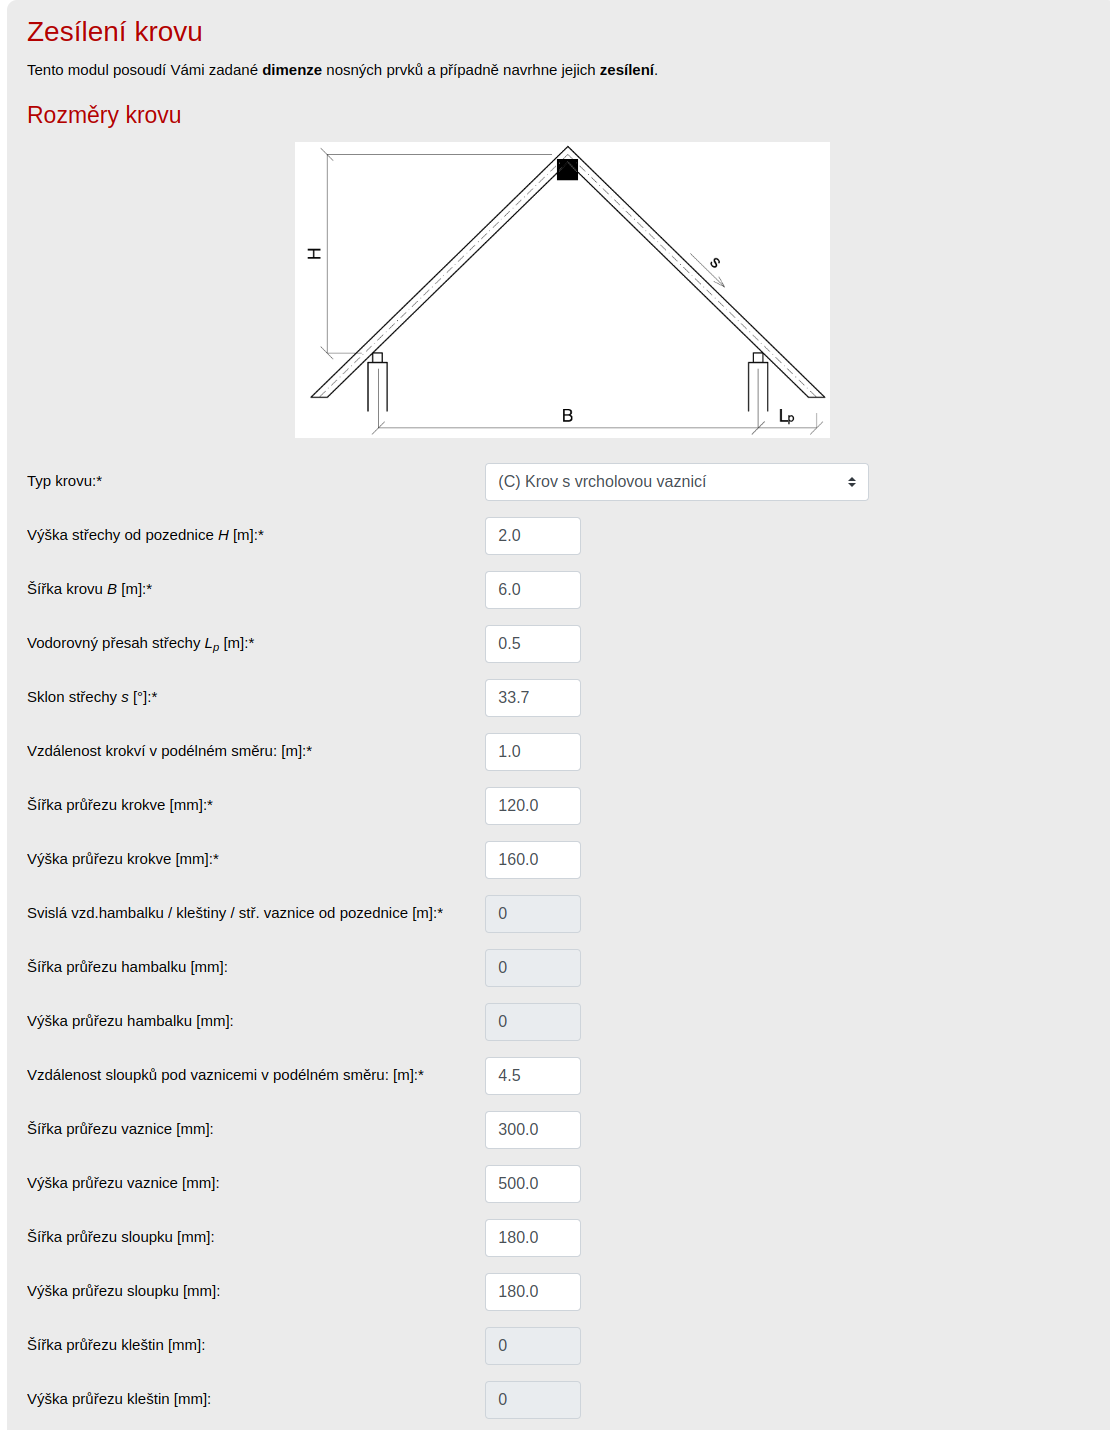
\includegraphics{assets/figures/wbapp/strecha_old-0-0.png}
    \caption{STŘECHA -- Modul pro finální posouzení 1/2}
    \label{fig:roof_old_1}
\end{figure}

\begin{figure}[H]
    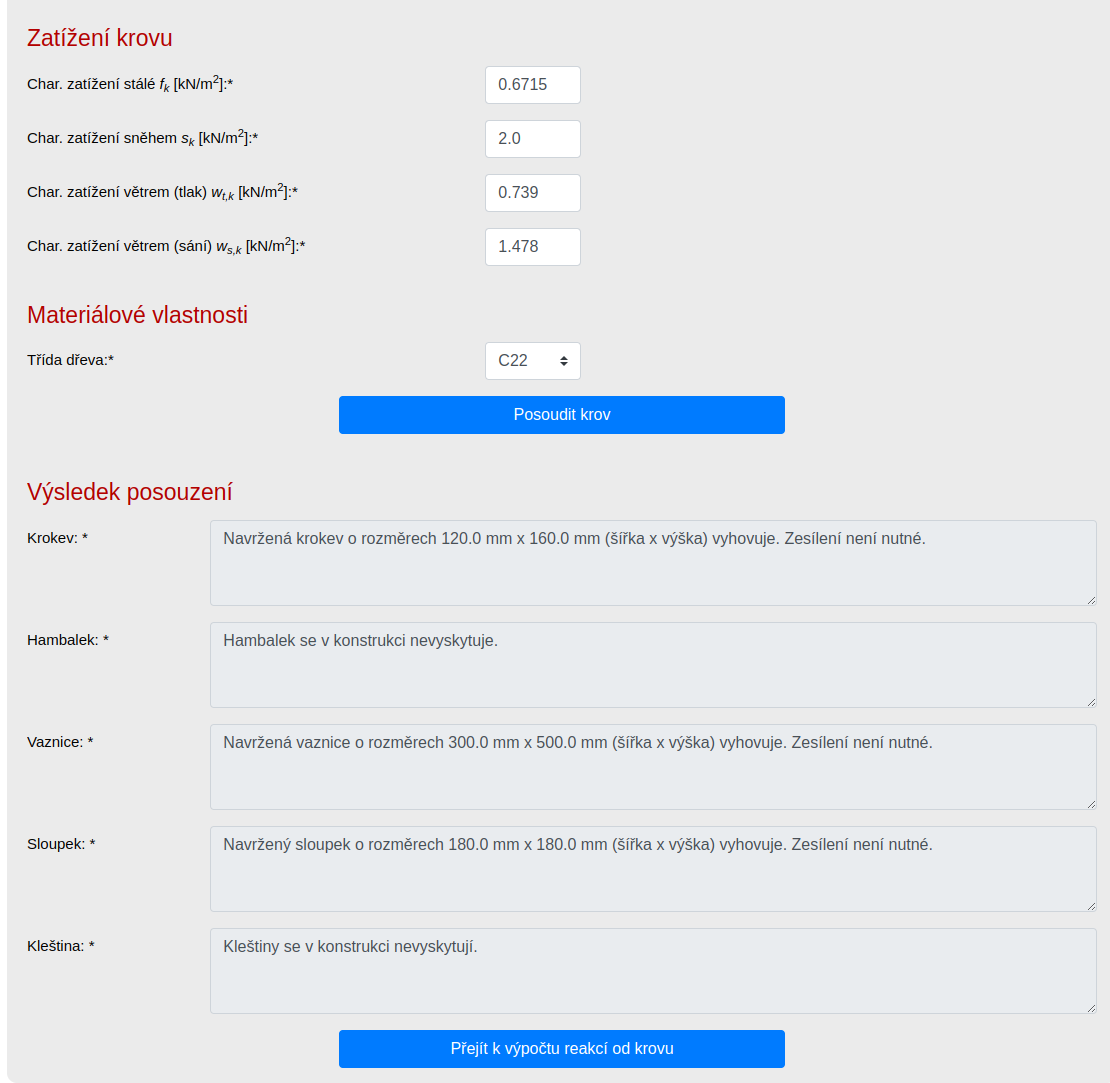
\includegraphics{assets/figures/wbapp/strecha_old-0-1.png}
    \caption{STŘECHA -- Modul pro finální posouzení 2/2}
    \label{fig:roof_old_2}
\end{figure}


\subsection{Nová verze}
Nová verze aplikace STŘECHA přináší výrazné zlepšení v uživatelském rozhraní a interaktivitě. Používá moderní technologie pro dynamickou vizualizaci a umožňuje uživatelům interaktivně modelovat střešní konstrukce.

\subsubsection*{Funkčnost}
Nová verze aplikace STŘECHA umožňuje uživatelům projít několika kroky k vygenerování statického schématu se zatíženími a zatěžovacími stavy, podobně jako tomu bylo v původní verzi. Nově však může měnit geometrii, přidávat a ubírat zatížení, definovat zatěžovací stavy, kombinovat je do kombinací a zobrazovat si výsledky pro jednotlivé stavy zvlášť.

Pro všechny tyto funkce aplikace využívá knihovny \texttt{framesss} a \texttt{desssign}, které byly představeny v předchozích kapitolách.

\subsubsection*{Uživatelské prostředí}
Nové uživatelské prostředí aplikace STŘECHA nabízí intuitivní a interaktivní rozhraní, které uživatelům umožňuje snadno zadávat data a mít nad nimi vizuální kontrolu.

V hlavní části obrazovky se nachází vizualizace modelu střechy, kde jsou zobrazeny uzly, prvky a aplikovaná zatížení. Uživatel může interaktivně přidávat uzly, prvky a zatížení pomocí ovládacích prvků v dolní části obrazovky. Tento přístup zajišťuje, že uživatelé mají přehled o všech zadaných datech a mohou je snadno upravovat a kontrolovat.

Uživatel může v prostředí aplikace:
\begin{itemize}
    \item generovat střešní konstrukci z předdefinovaných typů střešních konstrukcí,
    \item přidávat, editovat a mazat entity,
    \item vypočítat vnitřní síly,
    \item posoudit konstrukci.
\end{itemize}

\begin{figure}[H]
    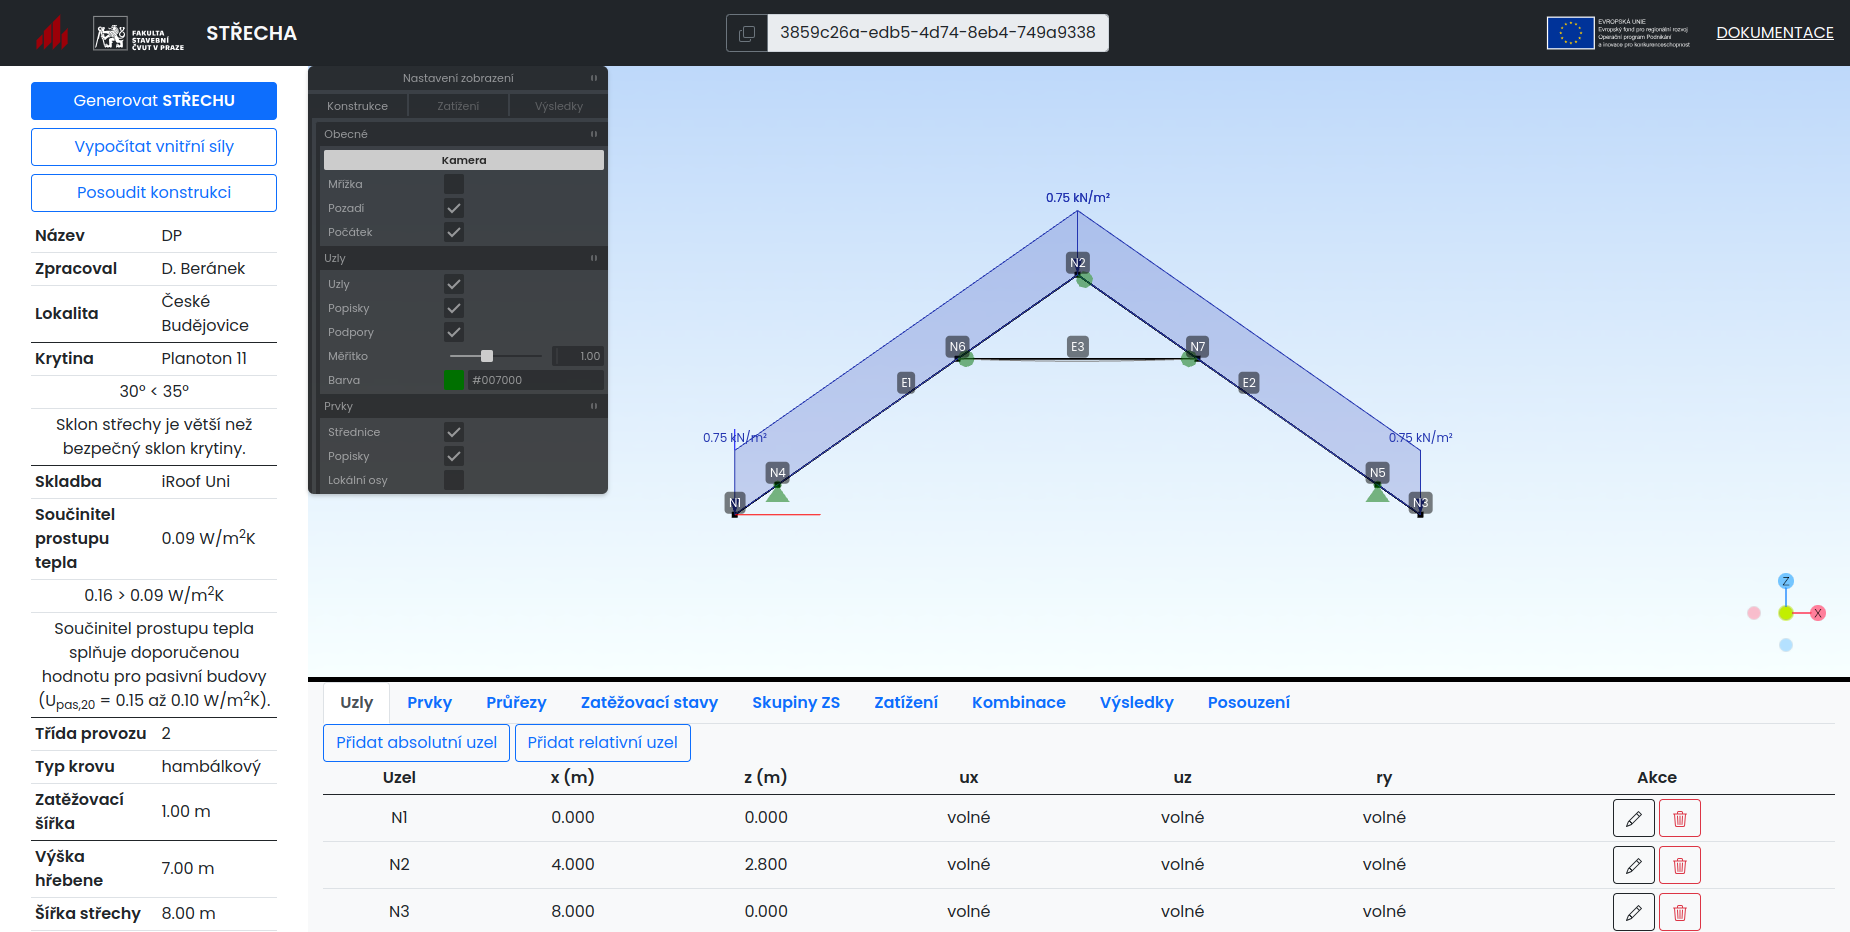
\includegraphics{assets/figures/wbapp/strecha_new.png}
    \caption{STŘECHA -- Nové uživatelské prostředí}
    \label{fig:roof_new}
\end{figure}

Na obrázku \autoref{fig:roof_new} je rozvržení nového uživatelského prostředí, na levé straně obrazovky se nachází panel s informacemi o projektu, jako je název, zpracovatel, lokalita, krytina, sklon střechy, skladba, součinitel prostupu tepla, typ krovu a další. V hlavní části obrazovky se nachází vizualizace statického modelu, kde jsou zobrazeny uzly, prvky a aplikovaná zatížení. Uživatel může interaktivně přidávat, měnit a mazat uzly, prvky, zatížení a veškeré další objekty pomocí ovládacích prvků v záložkách v dolní části obrazovky. Tento přístup zajišťuje, že uživatelé mají přehled o všech zadaných datech a mohou je snadno upravovat a kontrolovat.

\subsubsection*{Spodní panel}
V dolní části obrazovky se nachází karty s ovládacími prvky a přehlednými tabulkami, které zobrazují veškeré informace o modelované konstrukci. Tyto karty zahrnují:
\begin{itemize}
    \item \textbf{Uzly}: Seznam všech uzlů v modelu s jejich souřadnicemi a definicí podepření v jednotlivých směrech.
    \item \textbf{Prvky}: Seznam všech prvků, pro každý prvek se zde zobrazují jeho výchozí a koncový uzel, relativně zadané uzly, koncové klouby, délka a průřez.
    \item \textbf{Průřezy}: Seznam všech prvků s definicí materiálu a základních geometrických veličin.
    \item \textbf{Zatěžovací stavy}: Seznam všech zatěžovacích stavů, jejich typ, kategorie, třída trvání zatížení a odpovídající součinitele podle ČSN EN 1990.
    \item \textbf{Skupiny ZS}: Skupiny zatěžovacích stavů, ze kterých se generují kombinace.
    \item \textbf{Zatížení}: Seznam spojitých a bodových zatížení na prvcích a v uzlech. Na této kartě lze přepínat mezi zatěžovacími stavy. Zatížení pro aktivní zatěžovací stav se zobrazuje ve vizualizaci.
    \item \textbf{Kombinace}: Seznam všech kombinací, jejich mezní stav, typ a kombinační klíč.
    \item \textbf{Výsledky}: Seznam vnitřních sil ve všech průřezech, kde se může vyskytovat extrém vnitřních sil. Na této kartě lze přepínat mezi zatěžovacími stavy a kombinacemi zatížení. Pro aktivní výběr se vykreslují výsledky v modelu.
    \item \textbf{Posouzení}: Přehled využití jednotlivých prutů.
\end{itemize}

Na každé kartě je tlačítko pro přidání nové entity do modelu. Zároveň lze každou entitu, kromě zatížení vlastní tíhou, vymazat nebo upravit.

\begin{figure}[H]
    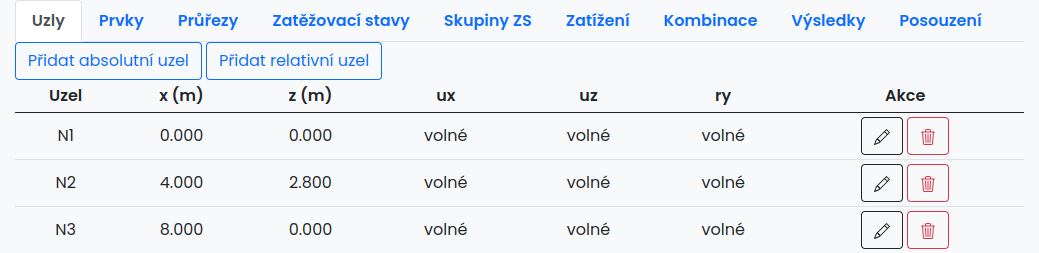
\includegraphics{assets/figures/wbapp/nodes_tab.png}
    \caption{STŘECHA -- Záložka s uzly}
    \label{fig:nodes}
\end{figure}

\begin{figure}[H]
    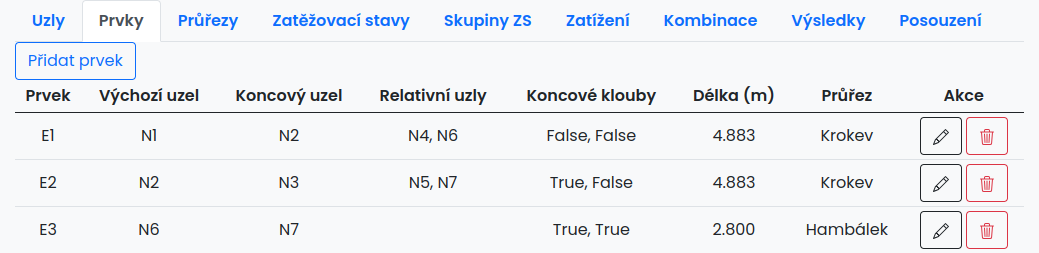
\includegraphics{assets/figures/wbapp/members_tab.png}
    \caption{STŘECHA -- Záložka s prvky}
    \label{fig:members}
\end{figure}

\begin{figure}[H]
    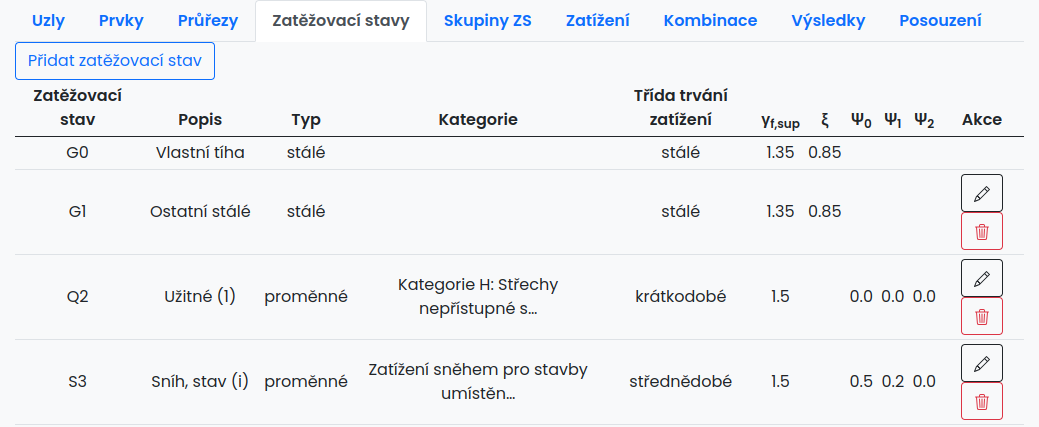
\includegraphics{assets/figures/wbapp/load_cases_tab.png}
    \caption{STŘECHA -- Záložka se zatěžovacími stavy}
    \label{fig:load_cases}
\end{figure}

\begin{figure}[H]
    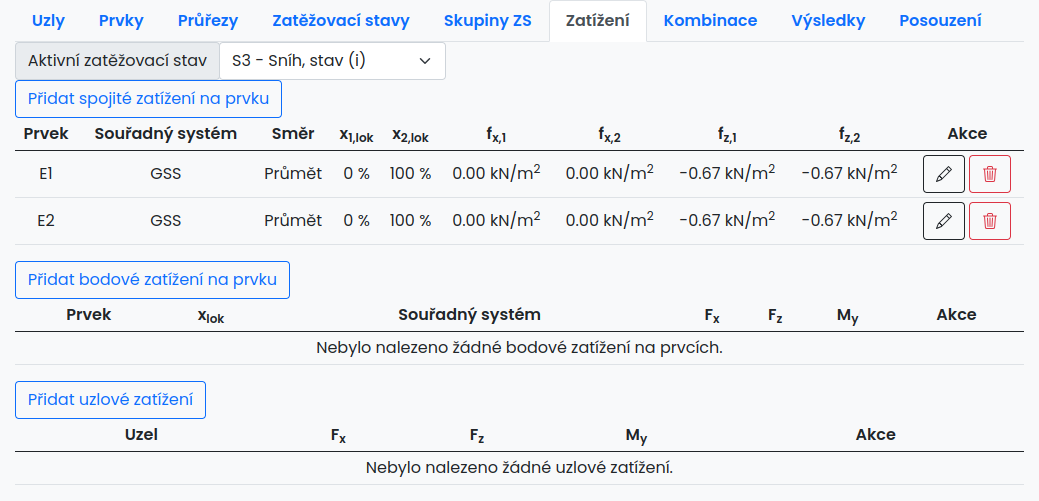
\includegraphics{assets/figures/wbapp/loads_tab.png}
    \caption{STŘECHA -- Záložka se zatížením}
    \label{fig:loads}
\end{figure}

\begin{figure}[H]
    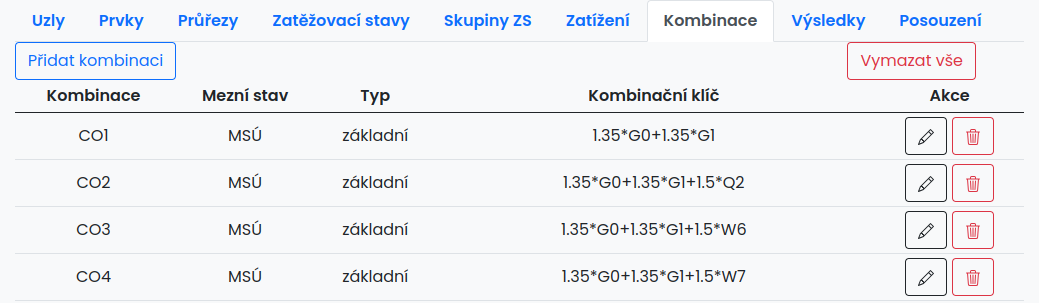
\includegraphics{assets/figures/wbapp/combos_tab.png}
    \caption{STŘECHA -- Záložka s kombinacemi zatížení}
    \label{fig:combos_tab}
\end{figure}

\subsubsection*{Editace entit}
Téměř každou entitu lze editovat. Po kliknutí na tlačítko \textbf{Přidat} nebo \textbf{Editovat} se zobrazí okno umožňující zadání potřebných údajů.
\begin{figure}[H]
    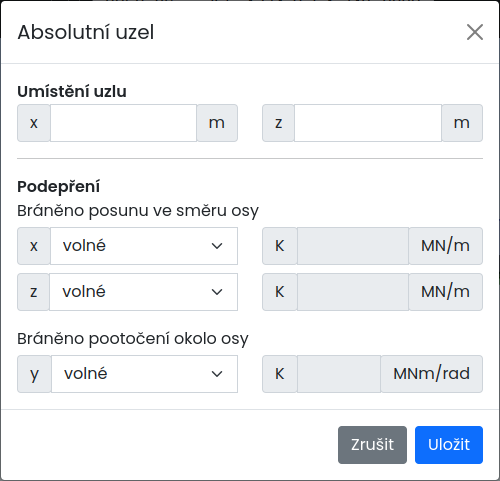
\includegraphics[width=7.5cm]{assets/figures/wbapp/add_node_modal.png}
    \caption{STŘECHA -- Okno pro přidání nového uzlu}
    \label{fig:add_node}
\end{figure}

\begin{figure}[H]
    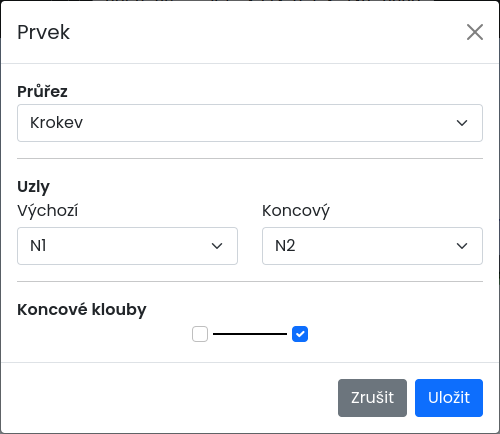
\includegraphics[width=7.5cm]{assets/figures/wbapp/add_member_modal.png}
    \caption{STŘECHA -- Okno pro přidání nového prvku}
    \label{fig:add_member}
\end{figure}

\begin{figure}[H]
    \includegraphics[width=7.5cm]{assets/figures/wbapp/add_load_Case_modal.png}
    \caption{STŘECHA -- Okno pro přidání nového zatěžovacího stavu}
    \label{fig:add_load_case}
\end{figure}


\chapter*{Shrnutí a diskuze}

Shrnutí celé diplomky, problémy/zajímavosti apd., diskuze příkladů\dots
\chapter*{Závěr a diskuze}
\pagestyle{plain}
V~první kapitole byly představeny základy teorie pružnosti, včetně veličin pro popis chování libovolného pružného tělesa a vztahů mezi nimi. Byl uveden princip virtuálních prací, ze kterého vychází princip virtuálních posunutí. Dále jsme se zabývali přibližným řešením úlohy dle teorie pružnosti, zobecněnými podmínkami rovnováhy a výpočtem matice tuhosti a vektoru zatížení. Poté jsme se zaměřili na 1D napjatost a popis pružného chování prutových prvků. Pomocí knihovny SymPy byly odvozeny matice tuhostí a vektory zatížení pro nejběžnější prutové prvky: tažený-tlačený prut, ohýbaný prut bez vlivu smyku a ohýbaný prut s~vlivem smyku. Následně byl představen princip statické kondenzace a transformace vztahů z~lokální do globální souřadné soustavy.

Dále byla představena objektově orientovaná knihovna pro výpočty prutových konstrukcí, vytvořená v~rámci této práce. Byly popsány externí open-source nástroje použité při vývoji, způsob instalace knihovny, včetně tvorby virtuálního prostředí, a jednotlivé funkce programu. Každý modul byl podrobně rozebrán a byly uvedeny obecné předpoklady přijaté při vývoji knihovny. Následně byl popsán algoritmus výpočtu celého modelu, použití řídkých matic a jejich implementace. Bylo také vysvětleno, jakým způsobem je knihovna testována, včetně významu unit testů a verifikačních testů. Jeden z~verifikačních testů byl detailně rozebrán v~prostředí JupyterLab, kde byly hodnoty porovnány s~referenčními hodnotami ze sbírky příkladů stavební mechaniky.

V~další kapitole byla představena knihovna pro navrhování konstrukcí podle Eurokódů, včetně instalace, architektury, detailního rozboru jednotlivých modulů a integrace s~knihovnou pro výpočty prutových konstrukcí. Byl uveden příklad použití pro vygenerování kombinací zatížení podle ČSN EN 1990.

V~poslední části byla představena webová aplikace vyvinutá v~rámci projektu \textit{Vývoj komplexního softwaru pro optimalizaci návrhu a posouzení střešních a stropních konstrukcí}, která prošla výrazným zlepšením funkčnosti. Nejprve byla představena aplikace STŘECHA, určená pro předběžný návrh konstrukčních prvků krovu se střešními krytinami a skladbami Tondach. Do aplikace STŘECHA bylo implementováno nové uživatelské prostředí a výpočetní nástroje představené v~prvních dvou kapitolách této práce. Byl znovu vyřešen příklad ze sbírky \cite{sbirka_prikladu} a porovnány výsledky s~referenčními průběhy vnitřních sil. Dále byla na krátkém případě předvedena funkčnost aplikace STROP.

V~rámci této diplomové práce bylo dosaženo několika významných cílů. Byly vyvinuty a verifikovány výpočetní nástroje (knihovny), které umožňují detailní analýzu prutových konstrukcí. Tyto nástroje lze použít pro analýzu jakýchkoliv prutových střešních a stropních konstrukcí. V~rámci práce bylo popsáno využití těchto knihoven pro zlepšení uživatelského rozhraní aplikace STŘECHA. Tato aplikace nyní představuje intuitivní a efektivní nástroj pro inženýry a projektanty. V~rámci pokračující práce na představené webové aplikaci budou tyto knihovny v~budoucnu integrovány i do aplikace STROP.

Hlavním přínosem jsou nově vytvořené knihovny pro analýzu prutových konstrukcí a vylepšení webové aplikace pro předběžné posouzení střešních a stropních konstrukcí. Neméně přínosný je i ucelený popis problematiky teorie pružnosti a představení knihovny SymPy pro symbolické výpočty.

Budoucí směřování práce zahrnuje dokončení integrace nově vytvořených knihoven do webové aplikace a tvorba nového uživatelského
rozhraní pro aplikaci STROP. Důležitým krokem bude také implementace dalších verifikačních testů a srovnání s~dalšími referenčními hodnotami.

\printbibliography

\end{document}
